\documentclass{beamer}
%
% Choose how your presentation looks.
%
% For more themes, color themes and font themes, see:
% http://deic.uab.es/~iblanes/beamer_gallery/index_by_theme.html
%
\mode<presentation>
{
  \usetheme{Warsaw}      % or try Darmstadt, Madrid, Warsaw, ...
  \usecolortheme{default} % or try albatross, beaver, crane, ...
  \usefonttheme{serif}  % or try serif, structurebold, ...
  %\setbeamertemplate{symbols}{}
  %\setbeamertemplate{caption}[numbered]
  \setbeamertemplate{navigation symbols}{}
  \setbeamertemplate{footline}{%
    \hfill\hspace{1cm}\insertframenumber{}/\inserttotalframenumber
  }
    \newenvironment{figure*}%
    {\begin{figure}}
    {\end{figure}}
    \newenvironment{table*}%
    {\begin{table}}
    {\end{table}}    
    \setbeamersize{text margin left=6mm, text margin right=2mm}
} 

\usepackage[english]{babel}
\usepackage[utf8x]{inputenc}
\usepackage{ifthen}
\usepackage{xspace}


% On writeLaTeX, these lines give you sharper preview images.
% You might want to comment them out before you export, though.
% \usepackage{pgfpages}

\newboolean{uprightparticles}
\setboolean{uprightparticles}{false} %True for upright particle symbols
%% %%%%%%%%%%%%%%%%%%%%%%%
%% Packages to be used
%% %%%%%%%%%%%%%%%%%%%%%%% 
\usepackage{microtype}
%\usepackage{lineno}  % for line numbering during review
\usepackage{xspace} % To avoid problems with missing or double spaces after
                    % predefined symbold

%% Graphics
\usepackage{graphicx}  % to include figures (can also use other packages)
\usepackage{color}
\usepackage{epic}
\usepackage{colortbl}
\usepackage{float}    % 
\usepackage{rotating}  % 
\usepackage{graphpap}  % 
\usepackage{multirow}  % 
\usepackage{cancel}    % 
\usefonttheme{professionalfonts}
\usepackage{times}
\usepackage{tikz}
\graphicspath{{figs/}} % Make Latex search fig subdir for figures

%% Math
\usepackage{amsmath} % Adds a large collection of math symbols
\usepackage{amssymb}
\usepackage{amsfonts}
\usepackage{upgreek} % Adds in support for greek letters in roman typeset

%% fix to allow peaceful coexistence of line numbering and
%% mathematical objects
%% http://www.latex-community.org/forum/viewtopic.php?f=5&t=163
%%
\newcommand*\patchAmsMathEnvironmentForLineno[1]{%
\expandafter\let\csname old#1\expandafter\endcsname\csname #1\endcsname
\expandafter\let\csname oldend#1\expandafter\endcsname\csname
end#1\endcsname
 \renewenvironment{#1}%
   {\linenomath\csname old#1\endcsname}%
   {\csname oldend#1\endcsname\endlinenomath}%
}
\newcommand*\patchBothAmsMathEnvironmentsForLineno[1]{%
  \patchAmsMathEnvironmentForLineno{#1}%
  \patchAmsMathEnvironmentForLineno{#1*}%
}
\AtBeginDocument{%
\patchBothAmsMathEnvironmentsForLineno{equation}%
\patchBothAmsMathEnvironmentsForLineno{align}%
\patchBothAmsMathEnvironmentsForLineno{flalign}%
\patchBothAmsMathEnvironmentsForLineno{alignat}%
\patchBothAmsMathEnvironmentsForLineno{gather}%
\patchBothAmsMathEnvironmentsForLineno{multline}%
}

% Get hyperlinks to captions and in references.
% These do not work with revtex. Use "hypertext" as class option instead.
\usepackage{hyperref}    % Hyperlinks in references
\usepackage[all]{hypcap} % Internal hyperlinks to floats.

%%% $Id: lhcb-symbols-def.tex 37234 2013-06-12 08:52:11Z roldeman $
%%% ======================================================================
%%% Purpose: Standard LHCb aliases
%%% Author: Originally Ulrik Egede, adapted by Tomasz Skwarnicki for templates,
%%% rewritten by Chris Parkes
%%% Maintainer : Ulrik Egede (2010 - 2012)
%%% =======================================================================

%%% To use this file outside the normal LHCb document environment, the
%%% following should be added in a preamble (before \begin{document}
%%%
%%%\usepackage{ifthen} 
%%%\newboolean{uprightparticles}
%%%\setboolean{uprightparticles}{false} %Set true for upright particle symbols
%%% \usepackage{xspace} 
%%% \usepackage{upgreek}

%%%%%%%%%%%%%%%%%%%%%%%%%%%%%%%%%%%%%%%%%%%%%%%%%%%%%%%%%%%%
%%%
%%% The following is to ensure that the template automatically can process
%%% this file.
%%%
%%% Add comments with at least three %%% preceding.
%%% Add new sections with one % preceding
%%% Add new subsections with two %% preceding
%%%%%%%%%%%%%%%%%%%%%%%%%%%%%%%%%%%%%%%%%%%%%%%%%%%%%%%%%%%%

%%%%%%%%%%%%%
% Experiments
%%%%%%%%%%%%%
\def\lhcb {\mbox{LHCb}\xspace}
\def\atlas  {\mbox{ATLAS}\xspace}
\def\cms    {\mbox{CMS}\xspace}
\def\alice  {\mbox{ALICE}\xspace}
\def\babar  {\mbox{BaBar}\xspace}
\def\belle  {\mbox{Belle}\xspace}
\def\cleo   {\mbox{CLEO}\xspace}
\def\cdf    {\mbox{CDF}\xspace}
\def\dzero  {\mbox{D0}\xspace}
\def\aleph  {\mbox{ALEPH}\xspace}
\def\delphi {\mbox{DELPHI}\xspace}
\def\opal   {\mbox{OPAL}\xspace}
\def\lthree {\mbox{L3}\xspace}
\def\sld    {\mbox{SLD}\xspace}
%%%\def\argus  {\mbox{ARGUS}\xspace}
%%%\def\uaone  {\mbox{UA1}\xspace}
%%%\def\uatwo  {\mbox{UA2}\xspace}
%%%\def\ux85 {\mbox{UX85}\xspace}
\def\cern {\mbox{CERN}\xspace}
\def\lhc    {\mbox{LHC}\xspace}
\def\lep    {\mbox{LEP}\xspace}
\def\tevatron {Tevatron\xspace}

%% LHCb sub-detectors and sub-systems

%%%\def\pu     {PU\xspace}
\def\velo   {VELO\xspace}
\def\rich   {RICH\xspace}
\def\richone {RICH1\xspace}
\def\richtwo {RICH2\xspace}
\def\ttracker {TT\xspace}
\def\intr   {IT\xspace}
\def\st     {ST\xspace}
\def\ot     {OT\xspace}
%%%\def\Tone   {T1\xspace}
%%%\def\Ttwo   {T2\xspace}
%%%\def\Tthree {T3\xspace}
%%%\def\Mone   {M1\xspace}
%%%\def\Mtwo   {M2\xspace}
%%%\def\Mthree {M3\xspace}
%%%\def\Mfour  {M4\xspace}
%%%\def\Mfive  {M5\xspace}
\def\spd    {SPD\xspace}
\def\presh  {PS\xspace}
\def\ecal   {ECAL\xspace}
\def\hcal   {HCAL\xspace}
%%%\def\bcm    {BCM\xspace}

%%%\def\ode    {ODE\xspace}
%%%\def\daq    {DAQ\xspace}
%%%\def\tfc    {TFC\xspace}
%%%\def\ecs    {ECS\xspace}
%%%\def\lone   {L0\xspace}
%%%\def\hlt    {HLT\xspace}
%%%\def\hltone {HLT1\xspace}
%%%\def\hlttwo {HLT2\xspace}

%%% Upright (not slanted) Particles

\ifthenelse{\boolean{uprightparticles}}%
{\def\Palpha      {\ensuremath{\upalpha}\xspace}
 \def\Pbeta       {\ensuremath{\upbeta}\xspace}
 \def\Pgamma      {\ensuremath{\upgamma}\xspace}                 
 \def\Pdelta      {\ensuremath{\updelta}\xspace}                 
 \def\Pepsilon    {\ensuremath{\upepsilon}\xspace}                 
 \def\Pvarepsilon {\ensuremath{\upvarepsilon}\xspace}                 
 \def\Pzeta       {\ensuremath{\upzeta}\xspace}                 
 \def\Peta        {\ensuremath{\upeta}\xspace}                 
 \def\Ptheta      {\ensuremath{\uptheta}\xspace}                 
 \def\Pvartheta   {\ensuremath{\upvartheta}\xspace}                 
 \def\Piota       {\ensuremath{\upiota}\xspace}                 
 \def\Pkappa      {\ensuremath{\upkappa}\xspace}                 
 \def\Plambda     {\ensuremath{\uplambda}\xspace}                 
 \def\Pmu         {\ensuremath{\upmu}\xspace}                 
 \def\Pnu         {\ensuremath{\upnu}\xspace}                 
 \def\Pxi         {\ensuremath{\upxi}\xspace}                 
 \def\Ppi         {\ensuremath{\uppi}\xspace}                 
 \def\Pvarpi      {\ensuremath{\upvarpi}\xspace}                 
 \def\Prho        {\ensuremath{\uprho}\xspace}                 
 \def\Pvarrho     {\ensuremath{\upvarrho}\xspace}                 
 \def\Ptau        {\ensuremath{\uptau}\xspace}                 
 \def\Pupsilon    {\ensuremath{\upupsilon}\xspace}                 
 \def\Pphi        {\ensuremath{\upphi}\xspace}                 
 \def\Pvarphi     {\ensuremath{\upvarphi}\xspace}                 
 \def\Pchi        {\ensuremath{\upchi}\xspace}                 
 \def\Ppsi        {\ensuremath{\uppsi}\xspace}                 
 \def\Pomega      {\ensuremath{\upomega}\xspace}                 

 \def\PDelta      {\ensuremath{\Delta}\xspace}                 
 \def\PXi      {\ensuremath{\Xi}\xspace}                 
 \def\PLambda      {\ensuremath{\Lambda}\xspace}                 
 \def\PSigma      {\ensuremath{\Sigma}\xspace}                 
 \def\POmega      {\ensuremath{\Omega}\xspace}                 
 \def\PUpsilon      {\ensuremath{\Upsilon}\xspace}                 
 
 %\mathchardef\Deltares="7101
 %\mathchardef\Xi="7104
 %\mathchardef\Lambda="7103
 %\mathchardef\Sigma="7106
 %\mathchardef\Omega="710A


 \def\PA      {\ensuremath{\mathrm{A}}\xspace}                 
 \def\PB      {\ensuremath{\mathrm{B}}\xspace}                 
 \def\PC      {\ensuremath{\mathrm{C}}\xspace}                 
 \def\PD      {\ensuremath{\mathrm{D}}\xspace}                 
 \def\PE      {\ensuremath{\mathrm{E}}\xspace}                 
 \def\PF      {\ensuremath{\mathrm{F}}\xspace}                 
 \def\PG      {\ensuremath{\mathrm{G}}\xspace}                 
 \def\PH      {\ensuremath{\mathrm{H}}\xspace}                 
 \def\PI      {\ensuremath{\mathrm{I}}\xspace}                 
 \def\PJ      {\ensuremath{\mathrm{J}}\xspace}                 
 \def\PK      {\ensuremath{\mathrm{K}}\xspace}                 
 \def\PL      {\ensuremath{\mathrm{L}}\xspace}                 
 \def\PM      {\ensuremath{\mathrm{M}}\xspace}                 
 \def\PN      {\ensuremath{\mathrm{N}}\xspace}                 
 \def\PO      {\ensuremath{\mathrm{O}}\xspace}                 
 \def\PP      {\ensuremath{\mathrm{P}}\xspace}                 
 \def\PQ      {\ensuremath{\mathrm{Q}}\xspace}                 
 \def\PR      {\ensuremath{\mathrm{R}}\xspace}                 
 \def\PS      {\ensuremath{\mathrm{S}}\xspace}                 
 \def\PT      {\ensuremath{\mathrm{T}}\xspace}                 
 \def\PU      {\ensuremath{\mathrm{U}}\xspace}                 
 \def\PV      {\ensuremath{\mathrm{V}}\xspace}                 
 \def\PW      {\ensuremath{\mathrm{W}}\xspace}                 
 \def\PX      {\ensuremath{\mathrm{X}}\xspace}                 
 \def\PY      {\ensuremath{\mathrm{Y}}\xspace}                 
 \def\PZ      {\ensuremath{\mathrm{Z}}\xspace}                 
 \def\Pa      {\ensuremath{\mathrm{a}}\xspace}                 
 \def\Pb      {\ensuremath{\mathrm{b}}\xspace}                 
 \def\Pc      {\ensuremath{\mathrm{c}}\xspace}                 
 \def\Pd      {\ensuremath{\mathrm{d}}\xspace}                 
 \def\Pe      {\ensuremath{\mathrm{e}}\xspace}                 
 \def\Pf      {\ensuremath{\mathrm{f}}\xspace}                 
 \def\Pg      {\ensuremath{\mathrm{g}}\xspace}                 
 \def\Ph      {\ensuremath{\mathrm{h}}\xspace}                 
 \def\Pi      {\ensuremath{\mathrm{i}}\xspace}                 
 \def\Pj      {\ensuremath{\mathrm{j}}\xspace}                 
 \def\Pk      {\ensuremath{\mathrm{k}}\xspace}                 
 \def\Pl      {\ensuremath{\mathrm{l}}\xspace}                 
 \def\Pm      {\ensuremath{\mathrm{m}}\xspace}                 
 \def\Pn      {\ensuremath{\mathrm{n}}\xspace}                 
 \def\Po      {\ensuremath{\mathrm{o}}\xspace}                 
 \def\Pp      {\ensuremath{\mathrm{p}}\xspace}                 
 \def\Pq      {\ensuremath{\mathrm{q}}\xspace}                 
 \def\Pr      {\ensuremath{\mathrm{r}}\xspace}                 
 \def\Ps      {\ensuremath{\mathrm{s}}\xspace}                 
 \def\Pt      {\ensuremath{\mathrm{t}}\xspace}                 
 \def\Pu      {\ensuremath{\mathrm{u}}\xspace}                 
 \def\Pv      {\ensuremath{\mathrm{v}}\xspace}                 
 \def\Pw      {\ensuremath{\mathrm{w}}\xspace}                 
 \def\Px      {\ensuremath{\mathrm{x}}\xspace}                 
 \def\Py      {\ensuremath{\mathrm{y}}\xspace}                 
 \def\Pz      {\ensuremath{\mathrm{z}}\xspace}                 
}
{\def\Palpha      {\ensuremath{\alpha}\xspace}
 \def\Pbeta       {\ensuremath{\beta}\xspace}
 \def\Pgamma      {\ensuremath{\gamma}\xspace}                 
 \def\Pdelta      {\ensuremath{\delta}\xspace}                 
 \def\Pepsilon    {\ensuremath{\epsilon}\xspace}                 
 \def\Pvarepsilon {\ensuremath{\varepsilon}\xspace}                 
 \def\Pzeta       {\ensuremath{\zeta}\xspace}                 
 \def\Peta        {\ensuremath{\eta}\xspace}                 
 \def\Ptheta      {\ensuremath{\theta}\xspace}                 
 \def\Pvartheta   {\ensuremath{\vartheta}\xspace}                 
 \def\Piota       {\ensuremath{\iota}\xspace}                 
 \def\Pkappa      {\ensuremath{\kappa}\xspace}                 
 \def\Plambda     {\ensuremath{\lambda}\xspace}                 
 \def\Pmu         {\ensuremath{\mu}\xspace}                 
 \def\Pnu         {\ensuremath{\nu}\xspace}                 
 \def\Pxi         {\ensuremath{\xi}\xspace}                 
 \def\Ppi         {\ensuremath{\pi}\xspace}                 
 \def\Pvarpi      {\ensuremath{\varpi}\xspace}                 
 \def\Prho        {\ensuremath{\rho}\xspace}                 
 \def\Pvarrho     {\ensuremath{\varrho}\xspace}                 
 \def\Ptau        {\ensuremath{\tau}\xspace}                 
 \def\Pupsilon    {\ensuremath{\upsilon}\xspace}                 
 \def\Pphi        {\ensuremath{\phi}\xspace}                 
 \def\Pvarphi     {\ensuremath{\varphi}\xspace}                 
 \def\Pchi        {\ensuremath{\chi}\xspace}                 
 \def\Ppsi        {\ensuremath{\psi}\xspace}                 
 \def\Pomega      {\ensuremath{\omega}\xspace}                 
 \mathchardef\PDelta="7101
 \mathchardef\PXi="7104
 \mathchardef\PLambda="7103
 \mathchardef\PSigma="7106
 \mathchardef\POmega="710A
 \mathchardef\PUpsilon="7107
 \def\PA      {\ensuremath{A}\xspace}                 
 \def\PB      {\ensuremath{B}\xspace}                 
 \def\PC      {\ensuremath{C}\xspace}                 
 \def\PD      {\ensuremath{D}\xspace}                 
 \def\PE      {\ensuremath{E}\xspace}                 
 \def\PF      {\ensuremath{F}\xspace}                 
 \def\PG      {\ensuremath{G}\xspace}                 
 \def\PH      {\ensuremath{H}\xspace}                 
 \def\PI      {\ensuremath{I}\xspace}                 
 \def\PJ      {\ensuremath{J}\xspace}                 
 \def\PK      {\ensuremath{K}\xspace}                 
 \def\PL      {\ensuremath{L}\xspace}                 
 \def\PM      {\ensuremath{M}\xspace}                 
 \def\PN      {\ensuremath{N}\xspace}                 
 \def\PO      {\ensuremath{O}\xspace}                 
 \def\PP      {\ensuremath{P}\xspace}                 
 \def\PQ      {\ensuremath{Q}\xspace}                 
 \def\PR      {\ensuremath{R}\xspace}                 
 \def\PS      {\ensuremath{S}\xspace}                 
 \def\PT      {\ensuremath{T}\xspace}                 
 \def\PU      {\ensuremath{U}\xspace}                 
 \def\PV      {\ensuremath{V}\xspace}                 
 \def\PW      {\ensuremath{W}\xspace}                 
 \def\PX      {\ensuremath{X}\xspace}                 
 \def\PY      {\ensuremath{Y}\xspace}                 
 \def\PZ      {\ensuremath{Z}\xspace}                 
 \def\Pa      {\ensuremath{a}\xspace}                 
 \def\Pb      {\ensuremath{b}\xspace}                 
 \def\Pc      {\ensuremath{c}\xspace}                 
 \def\Pd      {\ensuremath{d}\xspace}                 
 \def\Pe      {\ensuremath{e}\xspace}                 
 \def\Pf      {\ensuremath{f}\xspace}                 
 \def\Pg      {\ensuremath{g}\xspace}                 
 \def\Ph      {\ensuremath{h}\xspace}                 
 \def\Pi      {\ensuremath{i}\xspace}                 
 \def\Pj      {\ensuremath{j}\xspace}                 
 \def\Pk      {\ensuremath{k}\xspace}                 
 \def\Pl      {\ensuremath{l}\xspace}                 
 \def\Pm      {\ensuremath{m}\xspace}                 
 \def\Pn      {\ensuremath{n}\xspace}                 
 \def\Po      {\ensuremath{o}\xspace}                 
 \def\Pp      {\ensuremath{p}\xspace}                 
 \def\Pq      {\ensuremath{q}\xspace}                 
 \def\Pr      {\ensuremath{r}\xspace}                 
 \def\Ps      {\ensuremath{s}\xspace}                 
 \def\Pt      {\ensuremath{t}\xspace}                 
 \def\Pu      {\ensuremath{u}\xspace}                 
 \def\Pv      {\ensuremath{v}\xspace}                 
 \def\Pw      {\ensuremath{w}\xspace}                 
 \def\Px      {\ensuremath{x}\xspace}                 
 \def\Py      {\ensuremath{y}\xspace}                 
 \def\Pz      {\ensuremath{z}\xspace}                 
}

%%%%%%%%%%%%%%%%%%%%%%%%%%%%%%%%%%%%%%%%%%%%%%%
% Particles

%% Leptons

\let\emi\en
\def\electron   {\ensuremath{\Pe}\xspace}
\def\en         {\ensuremath{\Pe^-}\xspace}   % electron negative (\em is taken)
\def\ep         {\ensuremath{\Pe^+}\xspace}
\def\epm        {\ensuremath{\Pe^\pm}\xspace} 
\def\epem       {\ensuremath{\Pe^+\Pe^-}\xspace}
%%%\def\ee         {\ensuremath{\Pe^-\Pe^-}\xspace}

\def\mmu        {\ensuremath{\Pmu}\xspace}
\def\mup        {\ensuremath{\Pmu^+}\xspace}
\def\mun        {\ensuremath{\Pmu^-}\xspace} % muon negative (\mum is taken)
\def\mumu       {\ensuremath{\Pmu^+\Pmu^-}\xspace}
\def\mtau       {\ensuremath{\Ptau}\xspace}

\def\taup       {\ensuremath{\Ptau^+}\xspace}
\def\taum       {\ensuremath{\Ptau^-}\xspace}
\def\tautau     {\ensuremath{\Ptau^+\Ptau^-}\xspace}

\def\ellm       {\ensuremath{\ell^-}\xspace}
\def\ellp       {\ensuremath{\ell^+}\xspace}
%%%\def\ellell     {\ensuremath{\ell^+ \ell^-}\xspace}

\def\neu        {\ensuremath{\Pnu}\xspace}
\def\neub       {\ensuremath{\overline{\Pnu}}\xspace}
%%%\def\nuenueb    {\ensuremath{\neu\neub}\xspace}
\def\neue       {\ensuremath{\neu_e}\xspace}
\def\neueb      {\ensuremath{\neub_e}\xspace}
%%%\def\neueneueb  {\ensuremath{\neue\neueb}\xspace}
\def\neum       {\ensuremath{\neu_\mu}\xspace}
\def\neumb      {\ensuremath{\neub_\mu}\xspace}
%%%\def\neumneumb  {\ensuremath{\neum\neumb}\xspace}
\def\neut       {\ensuremath{\neu_\tau}\xspace}
\def\neutb      {\ensuremath{\neub_\tau}\xspace}
%%%\def\neutneutb  {\ensuremath{\neut\neutb}\xspace}
\def\neul       {\ensuremath{\neu_\ell}\xspace}
\def\neulb      {\ensuremath{\neub_\ell}\xspace}
%%%\def\neulneulb  {\ensuremath{\neul\neulb}\xspace}

%% Gauge bosons and scalars

\def\g      {\ensuremath{\Pgamma}\xspace}
\def\H      {\ensuremath{\PH^0}\xspace}
\def\Hp     {\ensuremath{\PH^+}\xspace}
\def\Hm     {\ensuremath{\PH^-}\xspace}
\def\Hpm    {\ensuremath{\PH^\pm}\xspace}
\def\W      {\ensuremath{\PW}\xspace}
\def\Wp     {\ensuremath{\PW^+}\xspace}
\def\Wm     {\ensuremath{\PW^-}\xspace}
\def\Wpm    {\ensuremath{\PW^\pm}\xspace}
\def\Z      {\ensuremath{\PZ}\xspace}

%% Quarks

\def\quark     {\ensuremath{\Pq}\xspace}
\def\quarkbar  {\ensuremath{\overline \quark}\xspace}
\def\qqbar     {\ensuremath{\quark\quarkbar}\xspace}
\def\uquark    {\ensuremath{\Pu}\xspace}
\def\uquarkbar {\ensuremath{\overline \uquark}\xspace}
\def\uubar     {\ensuremath{\uquark\uquarkbar}\xspace}
\def\dquark    {\ensuremath{\Pd}\xspace}
\def\dquarkbar {\ensuremath{\overline \dquark}\xspace}
\def\ddbar     {\ensuremath{\dquark\dquarkbar}\xspace}
\def\squark    {\ensuremath{\Ps}\xspace}
\def\squarkbar {\ensuremath{\overline \squark}\xspace}
\def\ssbar     {\ensuremath{\squark\squarkbar}\xspace}
\def\cquark    {\ensuremath{\Pc}\xspace}
\def\cquarkbar {\ensuremath{\overline \cquark}\xspace}
\def\ccbar     {\ensuremath{\cquark\cquarkbar}\xspace}
\def\bquark    {\ensuremath{\Pb}\xspace}
\def\bquarkbar {\ensuremath{\overline \bquark}\xspace}
\def\bbbar     {\ensuremath{\bquark\bquarkbar}\xspace}
\def\tquark    {\ensuremath{\Pt}\xspace}
\def\tquarkbar {\ensuremath{\overline \tquark}\xspace}
\def\ttbar     {\ensuremath{\tquark\tquarkbar}\xspace}

%% Light mesons

\def\pion  {\ensuremath{\Ppi}\xspace}
\def\piz   {\ensuremath{\pion^0}\xspace}
\def\pizs  {\ensuremath{\pion^0\mbox\,\rm{s}}\xspace}
%%%\def\ppz   {\ensuremath{\pion^0\pion^0}\xspace}
\def\pip   {\ensuremath{\pion^+}\xspace}
\def\pim   {\ensuremath{\pion^-}\xspace}
%%%\def\pipi  {\ensuremath{\pion^+\pion^-}\xspace}
\def\pipm  {\ensuremath{\pion^\pm}\xspace}
\def\pimp  {\ensuremath{\pion^\mp}\xspace}

\def\kaon  {\ensuremath{\PK}\xspace}
%%% do NOT use ensuremath here
  \def\Kbar  {\kern 0.2em\overline{\kern -0.2em \PK}{}\xspace}
\def\Kb    {\ensuremath{\Kbar}\xspace}
\def\Kz    {\ensuremath{\kaon^0}\xspace}
\def\Kzb   {\ensuremath{\Kbar^0}\xspace}
%%%\def\KzKzb {\ensuremath{\Kz \kern -0.16em \Kzb}\xspace}
\def\Kp    {\ensuremath{\kaon^+}\xspace}
\def\Km    {\ensuremath{\kaon^-}\xspace}
\def\Kpm   {\ensuremath{\kaon^\pm}\xspace}
\def\Kmp   {\ensuremath{\kaon^\mp}\xspace}
%%%\def\KpKm  {\ensuremath{\Kp \kern -0.16em \Km}\xspace}
\def\KS    {\ensuremath{\kaon^0_{\rm\scriptscriptstyle S}}\xspace} 
\def\KL    {\ensuremath{\kaon^0_{\rm\scriptscriptstyle L}}\xspace} 
\def\Kstarz  {\ensuremath{\kaon^{*0}}\xspace}
\def\Kstarzb {\ensuremath{\Kbar^{*0}}\xspace}
\def\Kstar   {\ensuremath{\kaon^*}\xspace}
\def\Kstarb  {\ensuremath{\Kbar^*}\xspace}
\def\Kstarp  {\ensuremath{\kaon^{*+}}\xspace}
\def\Kstarm  {\ensuremath{\kaon^{*-}}\xspace}
\def\Kstarpm {\ensuremath{\kaon^{*\pm}}\xspace}
\def\Kstarmp {\ensuremath{\kaon^{*\mp}}\xspace}

\newcommand{\etapr}{\ensuremath{\Peta^{\prime}}\xspace}

%% Heavy mesons

%%% do NOT use ensuremath here
  \def\Dbar    {\kern 0.2em\overline{\kern -0.2em \PD}{}\xspace}
\def\D       {\ensuremath{\PD}\xspace}
\def\Db      {\ensuremath{\Dbar}\xspace}
\def\Dz      {\ensuremath{\D^0}\xspace}
\def\Dzb     {\ensuremath{\Dbar^0}\xspace}
%%%\def\DzDzb   {\ensuremath{\Dz {\kern -0.16em \Dzb}}\xspace}
\def\Dp      {\ensuremath{\D^+}\xspace}
\def\Dm      {\ensuremath{\D^-}\xspace}
\def\Dpm     {\ensuremath{\D^\pm}\xspace}
\def\Dmp     {\ensuremath{\D^\mp}\xspace}
%%%\def\DpDm    {\ensuremath{\Dp {\kern -0.16em \Dm}}\xspace}
\def\Dstar   {\ensuremath{\D^*}\xspace}
\def\Dstarb  {\ensuremath{\Dbar^*}\xspace}
\def\Dstarz  {\ensuremath{\D^{*0}}\xspace}
\def\Dstarzb {\ensuremath{\Dbar^{*0}}\xspace}
\def\Dstarp  {\ensuremath{\D^{*+}}\xspace}
\def\Dstarm  {\ensuremath{\D^{*-}}\xspace}
\def\Dstarpm {\ensuremath{\D^{*\pm}}\xspace}
\def\Dstarmp {\ensuremath{\D^{*\mp}}\xspace}
\def\Ds      {\ensuremath{\D^+_\squark}\xspace}
\def\Dsp     {\ensuremath{\D^+_\squark}\xspace}
\def\Dsm     {\ensuremath{\D^-_\squark}\xspace}
\def\Dspm    {\ensuremath{\D^{\pm}_\squark}\xspace}
\def\Dsmp    {\ensuremath{\D^{\mp}_\squark}\xspace}
\def\Dss     {\ensuremath{\D^{*+}_\squark}\xspace}
\def\Dssp    {\ensuremath{\D^{*+}_\squark}\xspace}
\def\Dssm    {\ensuremath{\D^{*-}_\squark}\xspace}
\def\Dsspm   {\ensuremath{\D^{*\pm}_\squark}\xspace}
\def\Dssmp   {\ensuremath{\D^{*\mp}_\squark}\xspace}

\def\B       {\ensuremath{\PB}\xspace}
%%% do NOT use ensuremath here
\def\Bbar    {\ensuremath{\kern 0.18em\overline{\kern -0.18em \PB}{}}\xspace}
\def\Bb      {\ensuremath{\Bbar}\xspace}
%%%\def\BBbar   {\ensuremath{\B\Bbar}\xspace} 
\def\Bz      {\ensuremath{\B^0}\xspace}
\def\Bzb     {\ensuremath{\Bbar^0}\xspace}
\def\Bu      {\ensuremath{\B^+}\xspace}
\def\Bub     {\ensuremath{\B^-}\xspace}
\def\Bp      {\ensuremath{\Bu}\xspace}
\def\Bm      {\ensuremath{\Bub}\xspace}
\def\Bpm     {\ensuremath{\B^\pm}\xspace}
\def\Bmp     {\ensuremath{\B^\mp}\xspace}
\def\Bd      {\ensuremath{\B^0}\xspace}
\def\Bs      {\ensuremath{\B^0_\squark}\xspace}
\def\Bsb     {\ensuremath{\Bbar^0_\squark}\xspace}
\def\Bdb     {\ensuremath{\Bbar^0}\xspace}
\def\Bc      {\ensuremath{\B_\cquark^+}\xspace}
\def\Bcp     {\ensuremath{\B_\cquark^+}\xspace}
\def\Bcm     {\ensuremath{\B_\cquark^-}\xspace}
\def\Bcpm    {\ensuremath{\B_\cquark^\pm}\xspace}

%% Onia

\def\jpsi     {\ensuremath{{\PJ\mskip -3mu/\mskip -2mu\Ppsi\mskip 2mu}}\xspace}
\def\psitwos  {\ensuremath{\Ppsi{(2S)}}\xspace}
\def\psiprpr  {\ensuremath{\Ppsi(3770)}\xspace}
\def\etac     {\ensuremath{\Peta_\cquark}\xspace}
\def\chiczero {\ensuremath{\Pchi_{\cquark 0}}\xspace}
\def\chicone  {\ensuremath{\Pchi_{\cquark 1}}\xspace}
\def\chictwo  {\ensuremath{\Pchi_{\cquark 2}}\xspace}
  %\mathchardef\Upsilon="7107
  \def\Y#1S{\ensuremath{\PUpsilon{(#1S)}}\xspace}% no space before {...}!
\def\OneS  {\Y1S}
\def\TwoS  {\Y2S}
\def\ThreeS{\Y3S}
\def\FourS {\Y4S}
\def\FiveS {\Y5S}

\def\chic  {\ensuremath{\Pchi_{c}}\xspace}

\def\chib {\ensuremath{\Pchi_{\bquark}}\xspace}
\def\chibzero {\ensuremath{\Pchi_{\bquark 0}}\xspace}
\def\chibone  {\ensuremath{\Pchi_{\bquark 1}}\xspace}
\def\chibtwo  {\ensuremath{\Pchi_{\bquark 2}}\xspace}

\def\chibOneP  {\ensuremath{\Pchi_{\bquark}(1P)}\xspace}
\def\chibTwoP  {\ensuremath{\Pchi_{\bquark}(2P)}\xspace}
\def\chibThreeP  {\ensuremath{\Pchi_{\bquark}(3P)}\xspace}

\def\chiboneOneP  {\ensuremath{\Pchi_{\bquark 1}(1P)}\xspace}
\def\chiboneTwoP  {\ensuremath{\Pchi_{\bquark 1}(2P)}\xspace}
\def\chiboneThreeP  {\ensuremath{\Pchi_{\bquark 1}(3P)}\xspace}

\def\chibtwoOneP  {\ensuremath{\Pchi_{\bquark 2}(1P)}\xspace}
\def\chibtwoTwoP  {\ensuremath{\Pchi_{\bquark 2}(2P)}\xspace}
\def\chibtwoThreeP  {\ensuremath{\Pchi_{\bquark 2}(3P)}\xspace}



%% Baryons

\def\proton      {\ensuremath{\Pp}\xspace}
\def\antiproton  {\ensuremath{\overline \proton}\xspace}
\def\neutron     {\ensuremath{\Pn}\xspace}
\def\antineutron {\ensuremath{\overline \neutron}\xspace}

\def\Deltares {\ensuremath{\PDelta}\xspace}
\def\Deltaresbar{\ensuremath{\overline \Deltares}\xspace}
\def\Xires {\ensuremath{\PXi}\xspace}
\def\Xiresbar{\ensuremath{\overline \Xires}\xspace}
\def\Lz {\ensuremath{\PLambda}\xspace}
\def\Lbar {\ensuremath{\kern 0.1em\overline{\kern -0.1em\PLambda}}\xspace}
\def\Lambdares {\ensuremath{\PLambda}\xspace}
\def\Lambdaresbar{\ensuremath{\Lbar}\xspace}
\def\Sigmares {\ensuremath{\PSigma}\xspace}
\def\Sigmaresbar{\ensuremath{\overline \Sigmares}\xspace}
\def\Omegares {\ensuremath{\POmega^-}\xspace}
\def\Omegaresbar{\ensuremath{\overline{\POmega}^+}\xspace}

%%% do NOT use ensuremath here
 % \def\Deltabar{\kern 0.25em\overline{\kern -0.25em \Deltares}{}\xspace}
 % \def\Sigbar{\kern 0.2em\overline{\kern -0.2em \Sigma}{}\xspace}
 % \def\Xibar{\kern 0.2em\overline{\kern -0.2em \Xi}{}\xspace}
 % \def\Obar{\kern 0.2em\overline{\kern -0.2em \Omega}{}\xspace}
 % \def\Nbar{\kern 0.2em\overline{\kern -0.2em N}{}\xspace}
 % \def\Xb{\kern 0.2em\overline{\kern -0.2em X}{}\xspace}

\def\Lb      {\ensuremath{\Lz^0_\bquark}\xspace}
\def\Lbbar   {\ensuremath{\Lbar^0_\bquark}\xspace}
\def\Lc      {\ensuremath{\Lz^+_\cquark}\xspace}
\def\Lcbar   {\ensuremath{\Lbar^-_\cquark}\xspace}

%%%%%%%%%%%%%%%%%%
% Physics symbols
%%%%%%%%%%%%%%%%%

%% Decays
\def\BF         {{\ensuremath{\cal B}\xspace}}
\def\BRvis      {{\ensuremath{\BR_{\rm{vis}}}}}
\def\BR         {\BF}
\newcommand{\decay}[2]{\ensuremath{#1\!\to #2}\xspace}         % {\Pa}{\Pb \Pc}
\def\ra                 {\ensuremath{\rightarrow}\xspace}
\def\to                 {\ensuremath{\rightarrow}\xspace}

%% Lifetimes
\newcommand{\tauBs}{\ensuremath{\tau_{\Bs}}\xspace}
\newcommand{\tauBd}{\ensuremath{\tau_{\Bd}}\xspace}
\newcommand{\tauBz}{\ensuremath{\tau_{\Bz}}\xspace}
\newcommand{\tauBu}{\ensuremath{\tau_{\Bp}}\xspace}
\newcommand{\tauDp}{\ensuremath{\tau_{\Dp}}\xspace}
\newcommand{\tauDz}{\ensuremath{\tau_{\Dz}}\xspace}
\newcommand{\tauL}{\ensuremath{\tau_{\rm L}}\xspace}
\newcommand{\tauH}{\ensuremath{\tau_{\rm H}}\xspace}

%% Masses
\newcommand{\mBd}{\ensuremath{m_{\Bd}}\xspace}
\newcommand{\mBp}{\ensuremath{m_{\Bp}}\xspace}
\newcommand{\mBs}{\ensuremath{m_{\Bs}}\xspace}
\newcommand{\mBc}{\ensuremath{m_{\Bc}}\xspace}
\newcommand{\mLb}{\ensuremath{m_{\Lb}}\xspace}

%% EW theory, groups
\def\grpsuthree {\ensuremath{\mathrm{SU}(3)}\xspace}
\def\grpsutw    {\ensuremath{\mathrm{SU}(2)}\xspace}
\def\grpuone    {\ensuremath{\mathrm{U}(1)}\xspace}

\def\ssqtw {\ensuremath{\sin^{2}\!\theta_{\mathrm{W}}}\xspace}
\def\csqtw {\ensuremath{\cos^{2}\!\theta_{\mathrm{W}}}\xspace}
\def\stw   {\ensuremath{\sin\theta_{\mathrm{W}}}\xspace}
\def\ctw   {\ensuremath{\cos\theta_{\mathrm{W}}}\xspace}
\def\ssqtwef {\ensuremath{{\sin}^{2}\theta_{\mathrm{W}}^{\mathrm{eff}}}\xspace}
\def\csqtwef {\ensuremath{{\cos}^{2}\theta_{\mathrm{W}}^{\mathrm{eff}}}\xspace}
\def\stwef {\ensuremath{\sin\theta_{\mathrm{W}}^{\mathrm{eff}}}\xspace}
\def\ctwef {\ensuremath{\cos\theta_{\mathrm{W}}^{\mathrm{eff}}}\xspace}
\def\gv    {\ensuremath{g_{\mbox{\tiny V}}}\xspace}
\def\ga    {\ensuremath{g_{\mbox{\tiny A}}}\xspace}

\def\order   {\ensuremath{\mathcal{O}}\xspace}
\def\ordalph {\ensuremath{\mathcal{O}(\alpha)}\xspace}
\def\ordalsq {\ensuremath{\mathcal{O}(\alpha^{2})}\xspace}
\def\ordalcb {\ensuremath{\mathcal{O}(\alpha^{3})}\xspace}

%% QCD parameters
\newcommand{\as}{\ensuremath{\alpha_s}\xspace}
\newcommand{\MSb}{\ensuremath{\overline{\mathrm{MS}}}\xspace}
\newcommand{\lqcd}{\ensuremath{\Lambda_{\mathrm{QCD}}}\xspace}
\def\qsq       {\ensuremath{q^2}\xspace}

%% CKM, CP violation

\def\eps   {\ensuremath{\varepsilon}\xspace}
\def\epsK  {\ensuremath{\varepsilon_K}\xspace}
\def\epsB  {\ensuremath{\varepsilon_B}\xspace}
\def\epsp  {\ensuremath{\varepsilon^\prime_K}\xspace}

\def\CP                {\ensuremath{C\!P}\xspace}
\def\CPT               {\ensuremath{C\!PT}\xspace}

\def\rhobar {\ensuremath{\overline \rho}\xspace}
\def\etabar {\ensuremath{\overline \eta}\xspace}

\def\Vud  {\ensuremath{|V_{\uquark\dquark}|}\xspace}
\def\Vcd  {\ensuremath{|V_{\cquark\dquark}|}\xspace}
\def\Vtd  {\ensuremath{|V_{\tquark\dquark}|}\xspace}
\def\Vus  {\ensuremath{|V_{\uquark\squark}|}\xspace}
\def\Vcs  {\ensuremath{|V_{\cquark\squark}|}\xspace}
\def\Vts  {\ensuremath{|V_{\tquark\squark}|}\xspace}
\def\Vub  {\ensuremath{|V_{\uquark\bquark}|}\xspace}
\def\Vcb  {\ensuremath{|V_{\cquark\bquark}|}\xspace}
\def\Vtb  {\ensuremath{|V_{\tquark\bquark}|}\xspace}

%% Oscillations

\newcommand{\dm}{\ensuremath{\Delta m}\xspace}
\newcommand{\dms}{\ensuremath{\Delta m_{\squark}}\xspace}
\newcommand{\dmd}{\ensuremath{\Delta m_{\dquark}}\xspace}
\newcommand{\DG}{\ensuremath{\Delta\Gamma}\xspace}
\newcommand{\DGs}{\ensuremath{\Delta\Gamma_{\squark}}\xspace}
\newcommand{\DGd}{\ensuremath{\Delta\Gamma_{\dquark}}\xspace}
\newcommand{\Gs}{\ensuremath{\Gamma_{\squark}}\xspace}
\newcommand{\Gd}{\ensuremath{\Gamma_{\dquark}}\xspace}

\newcommand{\MBq}{\ensuremath{M_{\B_\quark}}\xspace}
\newcommand{\DGq}{\ensuremath{\Delta\Gamma_{\quark}}\xspace}
\newcommand{\Gq}{\ensuremath{\Gamma_{\quark}}\xspace}
\newcommand{\dmq}{\ensuremath{\Delta m_{\quark}}\xspace}
\newcommand{\GL}{\ensuremath{\Gamma_{\rm L}}\xspace}
\newcommand{\GH}{\ensuremath{\Gamma_{\rm H}}\xspace}

\newcommand{\DGsGs}{\ensuremath{\Delta\Gamma_{\squark}/\Gamma_{\squark}}\xspace}
\newcommand{\Delm}{\mbox{$\Delta m $}\xspace}
\newcommand{\ACP}{\ensuremath{{\cal A}^{\CP}}\xspace}
\newcommand{\Adir}{\ensuremath{{\cal A}^{\rm dir}}\xspace}
\newcommand{\Amix}{\ensuremath{{\cal A}^{\rm mix}}\xspace}
\newcommand{\ADelta}{\ensuremath{{\cal A}^\Delta}\xspace}
\newcommand{\phid}{\ensuremath{\phi_{\dquark}}\xspace}
\newcommand{\sinphid}{\ensuremath{\sin\!\phid}\xspace}
\newcommand{\phis}{\ensuremath{\phi_{\squark}}\xspace}
\newcommand{\betas}{\ensuremath{\beta_{\squark}}\xspace}
\newcommand{\sbetas}{\ensuremath{\sigma(\beta_{\squark})}\xspace}
\newcommand{\stbetas}{\ensuremath{\sigma(2\beta_{\squark})}\xspace}
\newcommand{\stphis}{\ensuremath{\sigma(\phi_{\squark})}\xspace}
\newcommand{\sinphis}{\ensuremath{\sin\!\phis}\xspace}

%% Tagging
\newcommand{\edet}{{\ensuremath{\varepsilon_{\rm det}}}\xspace}
\newcommand{\erec}{{\ensuremath{\varepsilon_{\rm rec/det}}}\xspace}
\newcommand{\esel}{{\ensuremath{\varepsilon_{\rm sel/rec}}}\xspace}
\newcommand{\etrg}{{\ensuremath{\varepsilon_{\rm trg/sel}}}\xspace}
\newcommand{\etot}{{\ensuremath{\varepsilon_{\rm tot}}}\xspace}

\newcommand{\mistag}{\ensuremath{\omega}\xspace}
\newcommand{\wcomb}{\ensuremath{\omega^{\rm comb}}\xspace}
\newcommand{\etag}{{\ensuremath{\varepsilon_{\rm tag}}}\xspace}
\newcommand{\etagcomb}{{\ensuremath{\varepsilon_{\rm tag}^{\rm comb}}}\xspace}
\newcommand{\effeff}{\ensuremath{\varepsilon_{\rm eff}}\xspace}
\newcommand{\effeffcomb}{\ensuremath{\varepsilon_{\rm eff}^{\rm comb}}\xspace}
\newcommand{\efftag}{{\ensuremath{\etag(1-2\omega)^2}}\xspace}
\newcommand{\effD}{{\ensuremath{\etag D^2}}\xspace}

\newcommand{\etagprompt}{{\ensuremath{\varepsilon_{\rm tag}^{\rm Pr}}}\xspace}
\newcommand{\etagLL}{{\ensuremath{\varepsilon_{\rm tag}^{\rm LL}}}\xspace}

%% Key decay channels

\def\BdToKstmm    {\decay{\Bd}{\Kstarz\mup\mun}}
\def\BdbToKstmm   {\decay{\Bdb}{\Kstarzb\mup\mun}}

\def\BsToJPsiPhi  {\decay{\Bs}{\jpsi\phi}}
\def\BdToJPsiKst  {\decay{\Bd}{\jpsi\Kstarz}}
\def\BdbToJPsiKst {\decay{\Bdb}{\jpsi\Kstarzb}}

\def\BsPhiGam     {\decay{\Bs}{\phi \g}}
\def\BdKstGam     {\decay{\Bd}{\Kstarz \g}}

\def\BTohh        {\decay{\B}{\Ph^+ \Ph'^-}}
\def\BdTopipi     {\decay{\Bd}{\pip\pim}}
\def\BdToKpi      {\decay{\Bd}{\Kp\pim}}
\def\BsToKK       {\decay{\Bs}{\Kp\Km}}
\def\BsTopiK      {\decay{\Bs}{\pip\Km}}

%% Rare decays
\def\BdKstee  {\decay{\Bd}{\Kstarz\epem}}
\def\BdbKstee {\decay{\Bdb}{\Kstarzb\epem}}
\def\bsll     {\decay{\bquark}{\squark \ell^+ \ell^-}}
\def\AFB      {\ensuremath{A_{\mathrm{FB}}}\xspace}
\def\FL       {\ensuremath{F_{\mathrm{L}}}\xspace}
\def\AT#1     {\ensuremath{A_{\mathrm{T}}^{#1}}\xspace}           % 2
\def\btosgam  {\decay{\bquark}{\squark \g}}
\def\btodgam  {\decay{\bquark}{\dquark \g}}
\def\Bsmm     {\decay{\Bs}{\mup\mun}}
\def\Bdmm     {\decay{\Bd}{\mup\mun}}
\def\ctl       {\ensuremath{\cos{\theta_\ell}}\xspace}
\def\ctk       {\ensuremath{\cos{\theta_K}}\xspace}

%% Wilson coefficients and operators
\def\C#1      {\ensuremath{\mathcal{C}_{#1}}\xspace}                       % 9
\def\Cp#1     {\ensuremath{\mathcal{C}_{#1}^{'}}\xspace}                    % 7
\def\Ceff#1   {\ensuremath{\mathcal{C}_{#1}^{\mathrm{(eff)}}}\xspace}        % 9  
\def\Cpeff#1  {\ensuremath{\mathcal{C}_{#1}^{'\mathrm{(eff)}}}\xspace}       % 7
\def\Ope#1    {\ensuremath{\mathcal{O}_{#1}}\xspace}                       % 2
\def\Opep#1   {\ensuremath{\mathcal{O}_{#1}^{'}}\xspace}                    % 7

%% Charm

\def\xprime     {\ensuremath{x^{\prime}}\xspace}
\def\yprime     {\ensuremath{y^{\prime}}\xspace}
\def\ycp        {\ensuremath{y_{\CP}}\xspace}
\def\agamma     {\ensuremath{A_{\Gamma}}\xspace}
%%%\def\kpi        {\ensuremath{\PK\Ppi}\xspace}
%%%\def\kk         {\ensuremath{\PK\PK}\xspace}
%%%\def\dkpi       {\decay{\PD}{\PK\Ppi}}
%%%\def\dkk        {\decay{\PD}{\PK\PK}}
\def\dkpicf     {\decay{\Dz}{\Km\pip}}

%% QM
\newcommand{\bra}[1]{\ensuremath{\langle #1|}}             % {a}
\newcommand{\ket}[1]{\ensuremath{|#1\rangle}}              % {b}
\newcommand{\braket}[2]{\ensuremath{\langle #1|#2\rangle}} % {a}{b}

%%%%%%%%%%%%%%%%%%%%%%%%%%%%%%%%%%%%%%%%%%%%%%%%%%
% Units
%%%%%%%%%%%%%%%%%%%%%%%%%%%%%%%%%%%%%%%%%%%%%%%%%%
\newcommand{\unit}[1]{\ensuremath{\rm\,#1}\xspace}          % {kg}

%% Energy and momentum
% \newcommand{\tev}{\ifthenelse{\boolean{inbibliography}}{\ensuremath{~T\kern -0.05em eV}\xspace}{\ensuremath{\mathrm{\,Te\kern -0.1em V}}\xspace}}
\newcommand{\tev}{\ensuremath{\mathrm{\,Te\kern -0.1em V}}\xspace}
\newcommand{\gev}{\ensuremath{\mathrm{\,Ge\kern -0.1em V}}\xspace}
\newcommand{\mev}{\ensuremath{\mathrm{\,Me\kern -0.1em V}}\xspace}
\newcommand{\kev}{\ensuremath{\mathrm{\,ke\kern -0.1em V}}\xspace}
\newcommand{\ev}{\ensuremath{\mathrm{\,e\kern -0.1em V}}\xspace}
\newcommand{\gevc}{\ensuremath{{\mathrm{\,Ge\kern -0.1em V\!/}c}}\xspace}
\newcommand{\mevc}{\ensuremath{{\mathrm{\,Me\kern -0.1em V\!/}c}}\xspace}
\newcommand{\gevcc}{\ensuremath{{\mathrm{\,Ge\kern -0.1em V\!/}c^2}}\xspace}
\newcommand{\gevgevcccc}{\ensuremath{{\mathrm{\,Ge\kern -0.1em V^2\!/}c^4}}\xspace}
\newcommand{\mevcc}{\ensuremath{{\mathrm{\,Me\kern -0.1em V\!/}c^2}}\xspace}

%% Distance and area
\def\km   {\ensuremath{\rm \,km}\xspace}
\def\m    {\ensuremath{\rm \,m}\xspace}
\def\cm   {\ensuremath{\rm \,cm}\xspace}
\def\cma  {\ensuremath{{\rm \,cm}^2}\xspace}
\def\mm   {\ensuremath{\rm \,mm}\xspace}
\def\mma  {\ensuremath{{\rm \,mm}^2}\xspace}
\def\mum  {\ensuremath{\,\upmu\rm m}\xspace}
\def\muma {\ensuremath{\,\upmu\rm m^2}\xspace}
\def\nm   {\ensuremath{\rm \,nm}\xspace}
\def\fm   {\ensuremath{\rm \,fm}\xspace}
\def\barn{\ensuremath{\rm \,b}\xspace}
%%%\def\barnhyph{\ensuremath{\rm -b}\xspace}
\def\mbarn{\ensuremath{\rm \,mb}\xspace}
\def\mub{\ensuremath{\rm \,\upmu b}\xspace}
%%%\def\mbarnhyph{\ensuremath{\rm -mb}\xspace}
\def\nb {\ensuremath{\rm \,nb}\xspace}
\def\invnb {\ensuremath{\mbox{\,nb}^{-1}}\xspace}
\def\pb {\ensuremath{\rm \,pb}\xspace}
\def\invpb {\ensuremath{\mbox{\,pb}^{-1}}\xspace}
\def\fb   {\ensuremath{\mbox{\,fb}}\xspace}
\def\invfb   {\ensuremath{\mbox{\,fb}^{-1}}\xspace}

%% Time 
\def\sec  {\ensuremath{\rm {\,s}}\xspace}
\def\ms   {\ensuremath{{\rm \,ms}}\xspace}
\def\mus  {\ensuremath{\,\upmu{\rm s}}\xspace}
\def\ns   {\ensuremath{{\rm \,ns}}\xspace}
\def\ps   {\ensuremath{{\rm \,ps}}\xspace}
\def\fs   {\ensuremath{\rm \,fs}\xspace}

\def\mhz  {\ensuremath{{\rm \,MHz}}\xspace}
\def\khz  {\ensuremath{{\rm \,kHz}}\xspace}
\def\hz   {\ensuremath{{\rm \,Hz}}\xspace}

\def\invps{\ensuremath{{\rm \,ps^{-1}}}\xspace}

\def\yr   {\ensuremath{\rm \,yr}\xspace}
\def\hr   {\ensuremath{\rm \,hr}\xspace}

%% Temperature
\def\degc {\ensuremath{^\circ}{C}\xspace}
\def\degk {\ensuremath {\rm K}\xspace}

%% Material lengths, radiation
\def\Xrad {\ensuremath{X_0}\xspace}
\def\NIL{\ensuremath{\lambda_{int}}\xspace}
\def\mip {MIP\xspace}
\def\neutroneq {\ensuremath{\rm \,n_{eq}}\xspace}
\def\neqcmcm {\ensuremath{\rm \,n_{eq} / cm^2}\xspace}
\def\kRad {\ensuremath{\rm \,kRad}\xspace}
\def\MRad {\ensuremath{\rm \,MRad}\xspace}
\def\ci {\ensuremath{\rm \,Ci}\xspace}
\def\mci {\ensuremath{\rm \,mCi}\xspace}

%% Uncertainties
\def\sx    {\ensuremath{\sigma_x}\xspace}    
\def\sy    {\ensuremath{\sigma_y}\xspace}   
\def\sz    {\ensuremath{\sigma_z}\xspace}    

\newcommand{\stat}{\ensuremath{\mathrm{\,(stat)}}\xspace}
\newcommand{\syst}{\ensuremath{\mathrm{\,(syst)}}\xspace}

%% Maths

\def\order{{\ensuremath{\cal O}}\xspace}
\newcommand{\chisq}{\ensuremath{\chi^2}\xspace}
\newcommand{\chisqndf}{\ensuremath{\chi^2/\mathrm{ndf}}\xspace}
\newcommand{\chisqip}{\ensuremath{\chi^2_{\rm IP}}\xspace}
\newcommand{\chisqvs}{\ensuremath{\chi^2_{\rm VS}}\xspace}
\newcommand{\chisqvtx}{\ensuremath{\chi^2_{\rm vtx}}\xspace}

\def\deriv {\ensuremath{\mathrm{d}}}

\def\gsim{{~\raise.15em\hbox{$>$}\kern-.85em
          \lower.35em\hbox{$\sim$}~}\xspace}
\def\lsim{{~\raise.15em\hbox{$<$}\kern-.85em
          \lower.35em\hbox{$\sim$}~}\xspace}

\newcommand{\mean}[1]{\ensuremath{\left\langle #1 \right\rangle}} % {x}
\newcommand{\abs}[1]{\ensuremath{\left\|#1\right\|}} % {x}
\newcommand{\Real}{\ensuremath{\mathcal{R}e}\xspace}
\newcommand{\Imag}{\ensuremath{\mathcal{I}m}\xspace}

\def\PDF {PDF\xspace}

\def\sPlot{\mbox{\em sPlot}\xspace}
\def\sWeight{\mbox{\em sWeight}}
%%%%%%%%%%%%%%%%%%%%%%%%%%%%%%%%%%%%%%%%%%%%%%%%%%
% Kinematics
%%%%%%%%%%%%%%%%%%%%%%%%%%%%%%%%%%%%%%%%%%%%%%%%%%

%% Energy, Momenta
\def\Ebeam {\ensuremath{E_{\mbox{\tiny BEAM}}}\xspace}
\def\sqs   {\ensuremath{\protect\sqrt{s}}\xspace}

\def\ptot       {\mbox{$p$}\xspace}
\def\pt         {\mbox{$p_{\rm T}$}\xspace}
\def\et         {\mbox{$E_{\rm T}$}\xspace}
\def\mt         {\mbox{$M_{\rm T}$}\xspace}
\def\dpp        {\ensuremath{\Delta p/p}\xspace}

\newcommand{\dedx}{\ensuremath{\mathrm{d}\hspace{-0.1em}E/\mathrm{d}x}\xspace}

%% PID

\def\dllkpi     {\ensuremath{\mathrm{DLL}_{\kaon\pion}}\xspace}
\def\dllppi     {\ensuremath{\mathrm{DLL}_{\proton\pion}}\xspace}
\def\dllepi     {\ensuremath{\mathrm{DLL}_{\electron\pion}}\xspace}
\def\dllmupi    {\ensuremath{\mathrm{DLL}_{\mmu\pi}}\xspace}

%% Geometry
%%%\def\mphi       {\mbox{$\phi$}\xspace}
%%%\def\mtheta     {\mbox{$\theta$}\xspace}
%%%\def\ctheta     {\mbox{$\cos\theta$}\xspace}
%%%\def\stheta     {\mbox{$\sin\theta$}\xspace}
%%%\def\ttheta     {\mbox{$\tan\theta$}\xspace}

\def\degrees{\ensuremath{^{\circ}}\xspace}
\def\krad {\ensuremath{\rm \,krad}\xspace}
\def\mrad{\ensuremath{\rm \,mrad}\xspace}
\def\rad{\ensuremath{\rm \,rad}\xspace}

%% Accelerator
\def\betastar {\ensuremath{\beta^*}}
\newcommand{\lum} {\ensuremath{\mathcal{L}}\xspace}
\newcommand{\intlum}[1]{\ensuremath{\int\lum=#1\xspace}}  % {2 \,\invfb}

%%%%%%%%%%%%%%%%%%%%%%%%%%%%%%%%%%%%%%%%%%%%%%%%%%%%%%%%%%%%%%%%%%%%
% Software
%%%%%%%%%%%%%%%%%%%%%%%%%%%%%%%%%%%%%%%%%%%%%%%%%%%%%%%%%%%%%%%%%%%%

%% Programs
%%%\def\ansys      {\mbox{\textsc{Ansys}}\xspace}
\def\bcvegpy    {\mbox{\textsc{Bcvegpy}}\xspace}
\def\boole      {\mbox{\textsc{Boole}}\xspace}
\def\brunel     {\mbox{\textsc{Brunel}}\xspace}
\def\davinci    {\mbox{\textsc{DaVinci}}\xspace}
\def\dirac      {\mbox{\textsc{Dirac}}\xspace}
%%%\def\erasmus    {\mbox{\textsc{Erasmus}}\xspace}
\def\evtgen     {\mbox{\textsc{EvtGen}}\xspace}
\def\fewz       {\mbox{\textsc{Fewz}}\xspace}
\def\fluka      {\mbox{\textsc{Fluka}}\xspace}
\def\ganga      {\mbox{\textsc{Ganga}}\xspace}
%%%\def\garfield   {\mbox{\textsc{Garfield}}\xspace}
\def\gaudi      {\mbox{\textsc{Gaudi}}\xspace}
\def\gauss      {\mbox{\textsc{Gauss}}\xspace}
\def\geant      {\mbox{\textsc{Geant4}}\xspace}
\def\hepmc      {\mbox{\textsc{HepMC}}\xspace}
\def\herwig     {\mbox{\textsc{Herwig}}\xspace}
\def\moore      {\mbox{\textsc{Moore}}\xspace}
\def\photos     {\mbox{\textsc{Photos}}\xspace}
\def\powheg     {\mbox{\textsc{Powheg}}\xspace}
%%%\def\pyroot     {\mbox{\textsc{PyRoot}}\xspace}
\def\pythia     {\mbox{\textsc{Pythia}}\xspace}
\def\resbos     {\mbox{\textsc{ResBos}}\xspace}
\def\roofit     {\mbox{\textsc{RooFit}}\xspace}
\def\root       {\mbox{\textsc{Root}}\xspace}
\def\spice      {\mbox{\textsc{Spice}}\xspace}
%%%\def\tosca      {\mbox{\textsc{Tosca}}\xspace}
\def\urania     {\mbox{\textsc{Urania}}\xspace}

%% Languages
\def\cpp        {\mbox{\textsc{C\raisebox{0.1em}{{\footnotesize{++}}}}}\xspace}
%%%\def\python     {\mbox{\textsc{Python}}\xspace}
\def\ruby       {\mbox{\textsc{Ruby}}\xspace}
\def\fortran    {\mbox{\textsc{Fortran}}\xspace}
\def\svn        {\mbox{\textsc{SVN}}\xspace}

%% Data processing
\def\kbytes     {\ensuremath{{\rm \,kbytes}}\xspace}
\def\kbsps      {\ensuremath{{\rm \,kbytes/s}}\xspace}
\def\kbits      {\ensuremath{{\rm \,kbits}}\xspace}
\def\kbsps      {\ensuremath{{\rm \,kbits/s}}\xspace}
\def\mbsps      {\ensuremath{{\rm \,Mbits/s}}\xspace}
\def\mbytes     {\ensuremath{{\rm \,Mbytes}}\xspace}
\def\mbps       {\ensuremath{{\rm \,Mbyte/s}}\xspace}
\def\mbsps      {\ensuremath{{\rm \,Mbytes/s}}\xspace}
\def\gbsps      {\ensuremath{{\rm \,Gbits/s}}\xspace}
\def\gbytes     {\ensuremath{{\rm \,Gbytes}}\xspace}
\def\gbsps      {\ensuremath{{\rm \,Gbytes/s}}\xspace}
\def\tbytes     {\ensuremath{{\rm \,Tbytes}}\xspace}
\def\tbpy       {\ensuremath{{\rm \,Tbytes/yr}}\xspace}

\def\dst        {DST\xspace}

%%%%%%%%%%%%%%%%%%%%%%%%%%%
% Detector related
%%%%%%%%%%%%%%%%%%%%%%%%%%%

%% Detector technologies
\def\nonn {\ensuremath{\rm {\it{n^+}}\mbox{-}on\mbox{-}{\it{n}}}\xspace}
\def\ponn {\ensuremath{\rm {\it{p^+}}\mbox{-}on\mbox{-}{\it{n}}}\xspace}
\def\nonp {\ensuremath{\rm {\it{n^+}}\mbox{-}on\mbox{-}{\it{p}}}\xspace}
\def\cvd  {CVD\xspace}
\def\mwpc {MWPC\xspace}
\def\gem  {GEM\xspace}

%% Detector components, electronics
\def\tell1  {TELL1\xspace}
\def\ukl1   {UKL1\xspace}
\def\beetle {Beetle\xspace}
\def\otis   {OTIS\xspace}
\def\croc   {CROC\xspace}
\def\carioca {CARIOCA\xspace}
\def\dialog {DIALOG\xspace}
\def\sync   {SYNC\xspace}
\def\cardiac {CARDIAC\xspace}
\def\gol    {GOL\xspace}
\def\vcsel  {VCSEL\xspace}
\def\ttc    {TTC\xspace}
\def\ttcrx  {TTCrx\xspace}
\def\hpd    {HPD\xspace}
\def\pmt    {PMT\xspace}
\def\specs  {SPECS\xspace}
\def\elmb   {ELMB\xspace}
\def\fpga   {FPGA\xspace}
\def\plc    {PLC\xspace}
\def\rasnik {RASNIK\xspace}
\def\elmb   {ELMB\xspace}
\def\can    {CAN\xspace}
\def\lvds   {LVDS\xspace}
\def\ntc    {NTC\xspace}
\def\adc    {ADC\xspace}
\def\led    {LED\xspace}
\def\ccd    {CCD\xspace}
\def\hv     {HV\xspace}
\def\lv     {LV\xspace}
\def\pvss   {PVSS\xspace}
\def\cmos   {CMOS\xspace}
\def\fifo   {FIFO\xspace}
\def\ccpc   {CCPC\xspace}

%% Chemical symbols
\def\cfourften     {\ensuremath{\rm C_4 F_{10}}\xspace}
\def\cffour        {\ensuremath{\rm CF_4}\xspace}
\def\cotwo         {\ensuremath{\rm CO_2}\xspace} 
\def\csixffouteen  {\ensuremath{\rm C_6 F_{14}}\xspace} 
\def\mgftwo     {\ensuremath{\rm Mg F_2}\xspace} 
\def\siotwo     {\ensuremath{\rm SiO_2}\xspace} 

%%%%%%%%%%%%%%%
% Special Text 
%%%%%%%%%%%%%%%
\newcommand{\eg}{\mbox{\itshape e.g.}\xspace}
\newcommand{\ie}{\mbox{\itshape i.e.}\xspace}
\newcommand{\etal}{\mbox{\itshape et al.}\xspace}
\newcommand{\etc}{\mbox{\itshape etc.}\xspace}
\newcommand{\cf}{\mbox{\itshape cf.}\xspace}
\newcommand{\ffp}{\mbox{\itshape ff.}\xspace}
\newcommand{\vs}{\mbox{\itshape vs.}\xspace}
 % Add in the predefined LHCb symbols

% Make this the last packages you include before the \begin{document}
\usepackage{cite} % Allows for ranges in citations
\usepackage{mciteplus}

\usepackage{float}
\usepackage{caption}
\usepackage{subcaption}
\usepackage{booktabs}


\title[chib status report]{Study of $\chi_b$ production at \sqs=7 and 8 TeV}
\subtitle{LHCb  (CERN)}
\author{Sasha Mazurov}
\institute{University of Ferrara (Italy) \& CERN}
\date{16 December 2013}


\begin{document}

\begin{frame}
  \titlepage
\end{frame}

\begin{frame}{Motivation}

\frametitle{Motivation}
$b\bar{b}$ system, which can be produced in different spin configurations, is
ideal laboratory for QCD tests. It's like a hydrogen atom in QCD.
\begin{columns}[c]
\column{.4\textwidth}
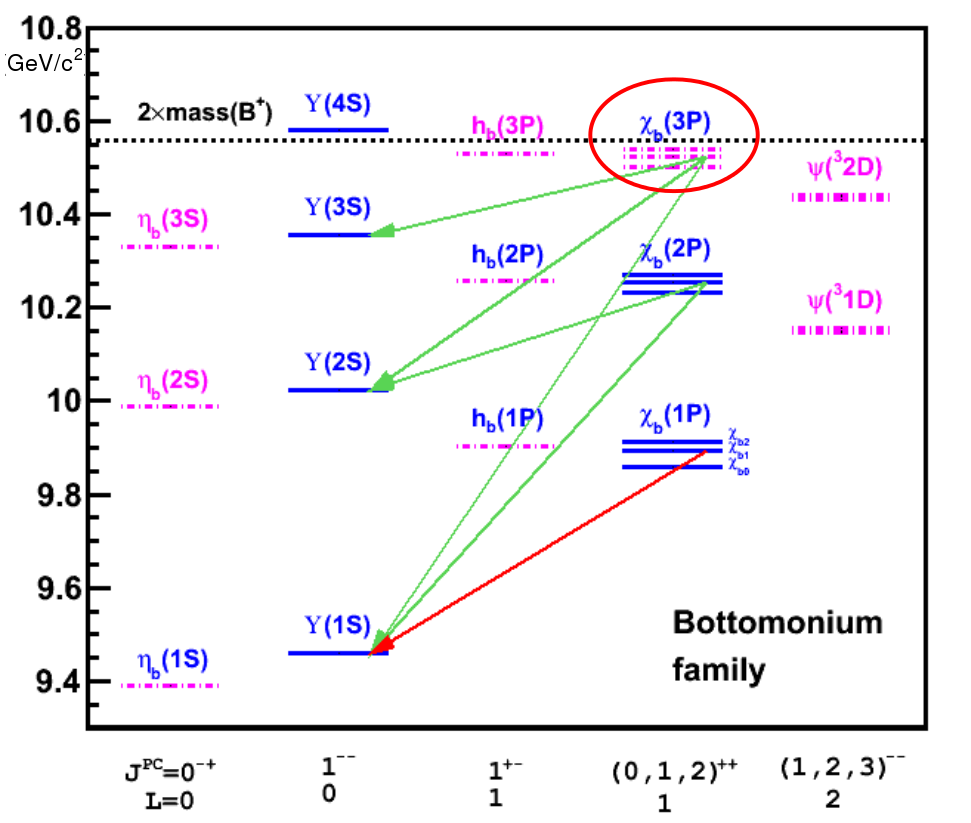
\includegraphics[width=\textwidth]{bfamily.png}
\begin{itemize}
  \item \textcolor{blue}{Measured mass}
  \item \textcolor{red}{Mass from theory}
\end{itemize}
\column{.6\textwidth}
\fontsize{9pt}{7.2}\selectfont
States with parallel quark spins (S=1):
\begin{itemize}
  \item S-wave $\Upsilon$ state.
  \item P-wave $\chi_{b}$ states, composed by 3 spin states $\chi_{b(0,1,2)}$. 
  \item $\Upsilon$ can be readily produced in the radiactive decays of $\chib$.
  \item $\chi_{b}(3P)$ state recently observed by ATLAS, D0 and LHCb.
\end{itemize}
Study of $\chi_{b}$ production:
\begin{enumerate}
  \item Measurement for $\Upsilon(NS)$ (N=1, 2, 3) cross sections in $\chi_b$
  decays as a function of $p_T(N\Upsilon)$
  \item Measurement of $\chi_{b(0,1,2)}(3P)$ mass.
\end{enumerate}
\end{columns}

\end{frame}
\begin{frame}{Previous analysis at LHCb}
\begin{itemize}
\item "Measurement of the fraction of $\Upsilon(1S)$ originating from $\chi_b(1P)$ in pp collisions at \sqs=7\tev", arXiv:1209.0282, \intlum{32} \invpb
\item "Observation of the $\chi_b(3P)$ state at LHCb in pp collisions at \sqs=7\tev",
LHCb-CONF-2012-020, \intlum{0.9} \invfb.
\end{itemize}
\end{frame}
\begin{frame}
\frametitle{Cross sections formula}
In each $p_T(\Upsilon)$ bin calculate:
\begin{center}
$\frac{\sigma(\chi_{b} \rightarrow \Upsilon \gamma)}{\sigma(\Upsilon)} = \frac{N_{\chi_b \rightarrow \Upsilon \gamma}}{N_{\Upsilon}} \times \frac{\epsilon_{\Upsilon}}{\epsilon_{\chi_b \rightarrow \Upsilon \gamma}} = \frac{N_{\chi_b \rightarrow \Upsilon \gamma}}{N_{\Upsilon}} \times \frac{1}{\epsilon_{\gamma}^{reco}}$
\end{center}
\begin{itemize}
  \item Calculate for each $\Upsilon(nS), n=1,2,3$ and $\chi_b(mP), m=1,2,3$
  \item Get N from fits: $N_{\Upsilon}$ from  $m(\mu^+ \mu^-)$ and $N_{\chi_b \rightarrow \Upsilon \gamma}$ from [$m(\mu^+ \mu^- \gamma) - m(\mu^+ \mu^-)$] (for better resolution)
  \item Compute efficiency $\epsilon$  from Monte-Carlo simulation
\end{itemize}
\end{frame}
\begin{frame}{Plan}
\begin{enumerate}
\item Datasets
\item Determination of $\Upsilon$ yields
\item Determination of \chib yields in the following decays
\begin{itemize}
    \item $\chi_b(1,2,3P) \to \OneS \gamma$
    \item $\chi_b(2,3P) \to \TwoS \gamma$
    \item $\chi_b(3P) \to \ThreeS \gamma$
\end{itemize}
\item Monte-Carlo efficiencies
\item The fraction of $\Upsilon$ originating from \chib decays.
\item Systematic uncertainties 
\end{enumerate}
\end{frame}

\begin{frame}{Datasets}
\begin{itemize}
\item Full 2011 dataset at \sqs=7\tev. \intlum{1} \invfb
\item Full 2012 dataset at \sqs=8\tev. \intlum{2} \invfb
\item Monte-Carlo simulation of \chib inclusive decays, generated
$62\times10^6$ events.
\end{itemize}
\end{frame}

\begin{frame}{The $\Upsilon$ selection}
\begin{center}
\scalebox{0.7}{
\begin{tabular}{cl}\toprule
Description & Requirement \\
\midrule
Track fit quality &  $\chisq/\rm{ndf} < 4$ \\
Track $p_T$ &  $> 1$ \gevc \\
Primary vertex probability & $> 0.5 \%$ \\
Luminous region &  $|z_{PV}| < 0.5 m$ and $x_{PV}^2 + y_{PV}^2 < 100 mm^2$ \\
Kullback-Leibler distance & $> 5000$ \\
\rule{0pt}{4ex}Muon and hadron hypotheses & $\Delta\log\lum^{\mmu-\Ph} > 0$ \\
Muon probability & ProbNN  $> 0.5$ \\
\multicolumn{2}{l}{\rule{0pt}{4ex}Trigger lines:} \\
L0 &  DiMuon.*Decision \\
HLT1 & Hlt1DiMuonHighMass.*Decision \\
HLT2 & HLT2DiMuonB.*Decision \\
\bottomrule
\end{tabular}
} % scale
\end{center}
\end{frame}


\begin{frame}{The $\Upsilon$ fit model}
\setlength{\unitlength}{1mm}
\begin{columns}
\column{.5\textwidth}
\scalebox{0.7}{
  \begin{picture}(75,60)
    \put(0,0){
      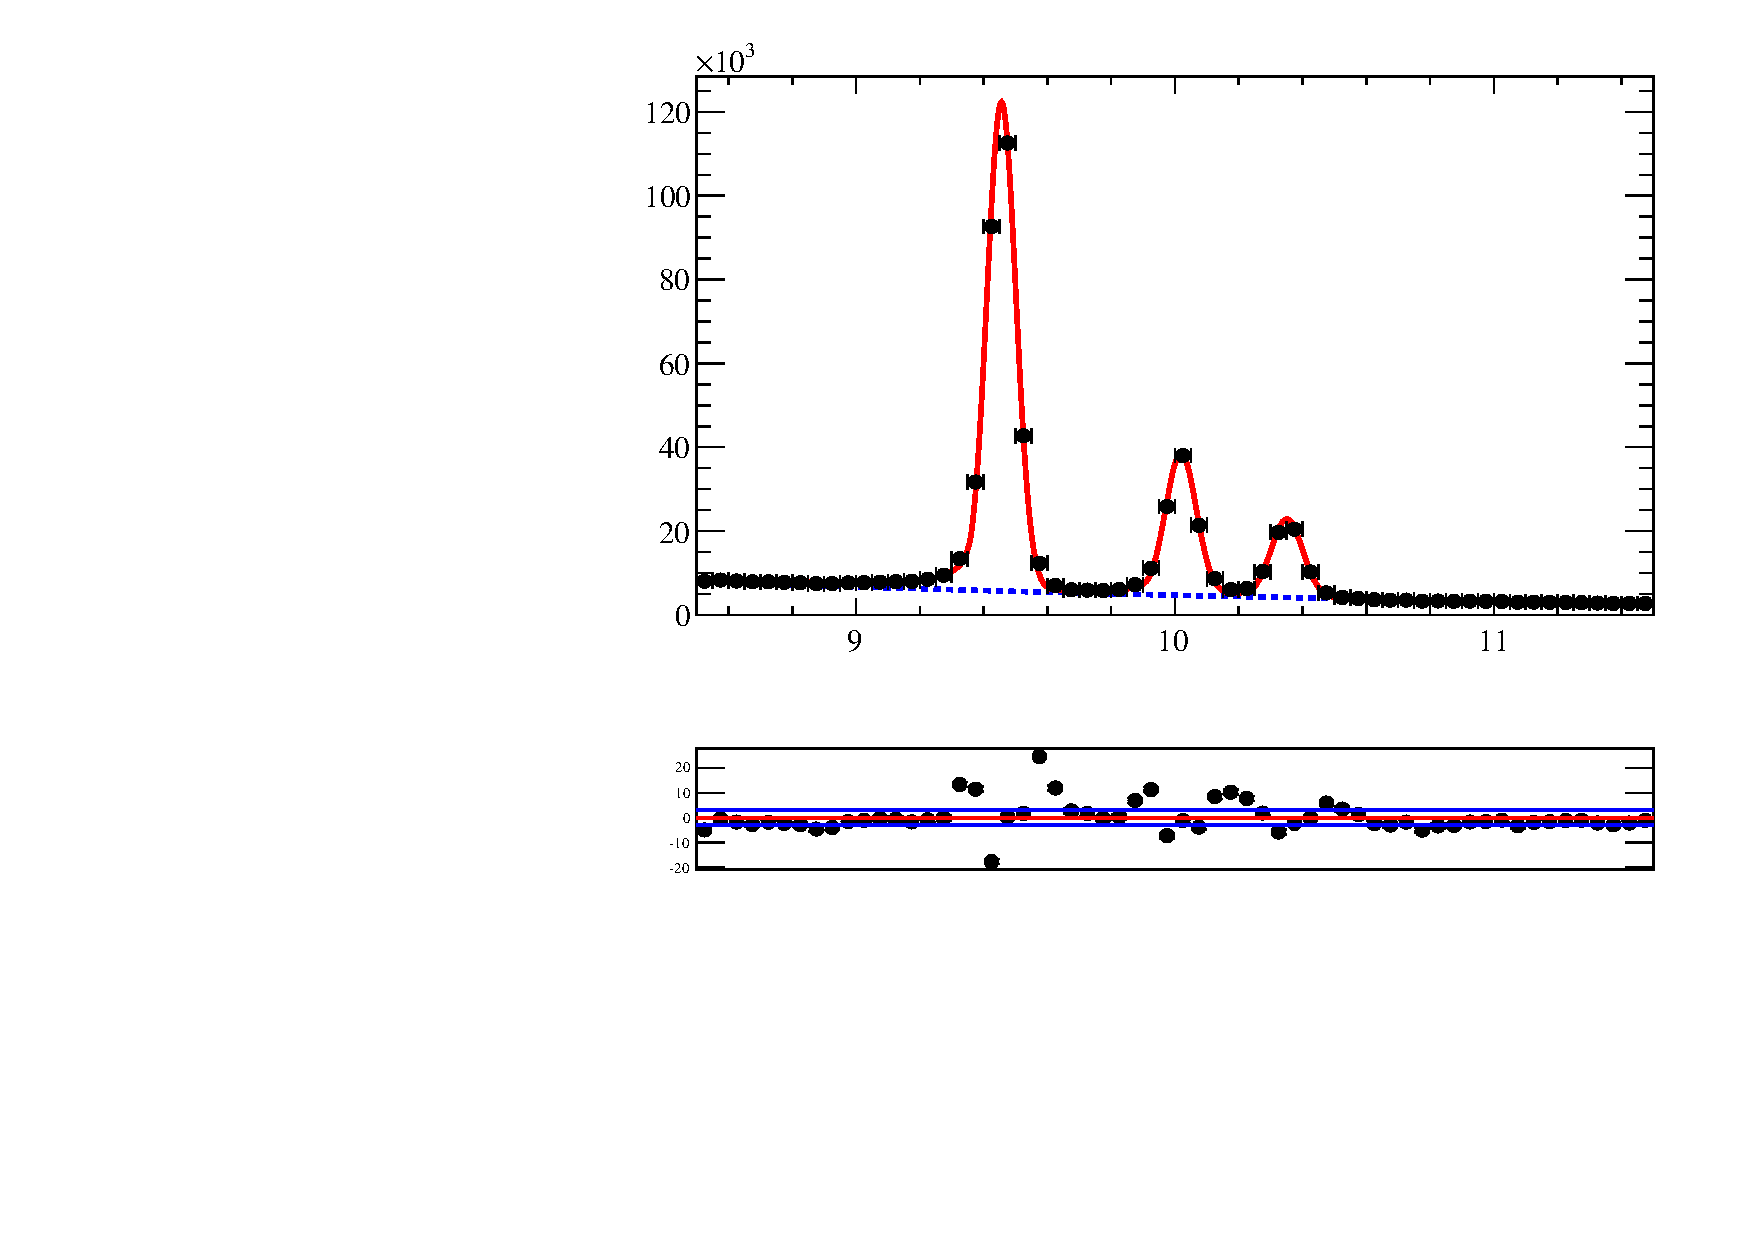
\includegraphics[width=75mm, height=60mm]{upsilon-fit/f2011_6_40}
    }
    \put(2,18){\small \begin{sideways}Candidates/(40\mevcc)\end{sideways}}
    \put(25, 13){$m_{\mumu} \left[\gevcc\right]$}
    \put(45,45){\sqs = 7 \tev}
    \put(35,38){$6 < p_T^{\mumu} < 40 \gevc$}
    % \graphpaper[5](0,0)(150, 60)
  \end{picture}
}
\begin{itemize}
\item 3 Crystal Ball functions for signal yields ($\alpha=2$, $n=5$).
\item Exponential function for combinatorial background.
\end{itemize}

\column{.5\textwidth}
\scalebox{0.5}{
    \begin{tabular}{lrrr}\toprule
    & \multicolumn{ 3 }{c}{$\mumu$ transverse momentum intervals (\gevc)} \\
     & & \multicolumn{2}{c}{6 --- 40} \\
    \cmidrule{3-4}
     && \sqs = 7 \tev & \sqs = 8\tev \\
    \midrule
    $N_{\Y1S}$ &&284,300 $\pm$ 600&661,800 $\pm$ 900 \\
    $N_{\Y2S}$ &&88,100 $\pm$ 400&204,800 $\pm$ 500 \\
    $N_{\Y3S}$ &&50,850 $\pm$ 290&116,700 $\pm$ 400 \\

    \rule{0pt}{4ex}$B$ &&294,300 $\pm$ 700&716,100 $\pm$ 1100 \\

    \rule{0pt}{4ex}$\mu_{\Y1S}, \mevcc$ &&9456.64 $\pm$ 0.09&9455.24 $\pm$ 0.06 \\
    % $\Delta m_{\Y2S}, \mevcc$ &&563.0&563.0 \\
    % $\Delta m_{\Y3S}, \mevcc$ &&894.9&894.9 \\

    \rule{0pt}{4ex}$\sigma_{\Y1S}, \mevcc$ &&45.23 $\pm$ 0.08&45.38 $\pm$ 0.06 \\

    % \rule{0pt}{4ex}$\alpha$ &&2.0&2.0 \\
    % $n$ &&1.0&1.0 \\

    % \rule{0pt}{4ex}$\tau$ &&-0.3574 $\pm$ 0.0023&-0.3526 $\pm$ 0.0015 \\

    % \rule{0pt}{4ex}$\chi^2/ndf$ &&24.9&49.5 \\    
    \bottomrule
    \end{tabular}   
}

\bigskip

\begin{itemize}
\item \Y1S mass is about 5 \mevcc lower than PDG value $9460.30 \pm  0.26$ \mevcc
\item In this study \OneS mass was fixed to $9.456 \gevcc$ 
\end{itemize}
\end{columns}


\end{frame}


\begin{frame}{$\Upsilon$ yields as function of $p_T$}
  \setlength{\unitlength}{1mm}
  \centering
  \scalebox{0.55 }{
  \begin{picture}(150,120)
    \put(0,0){
      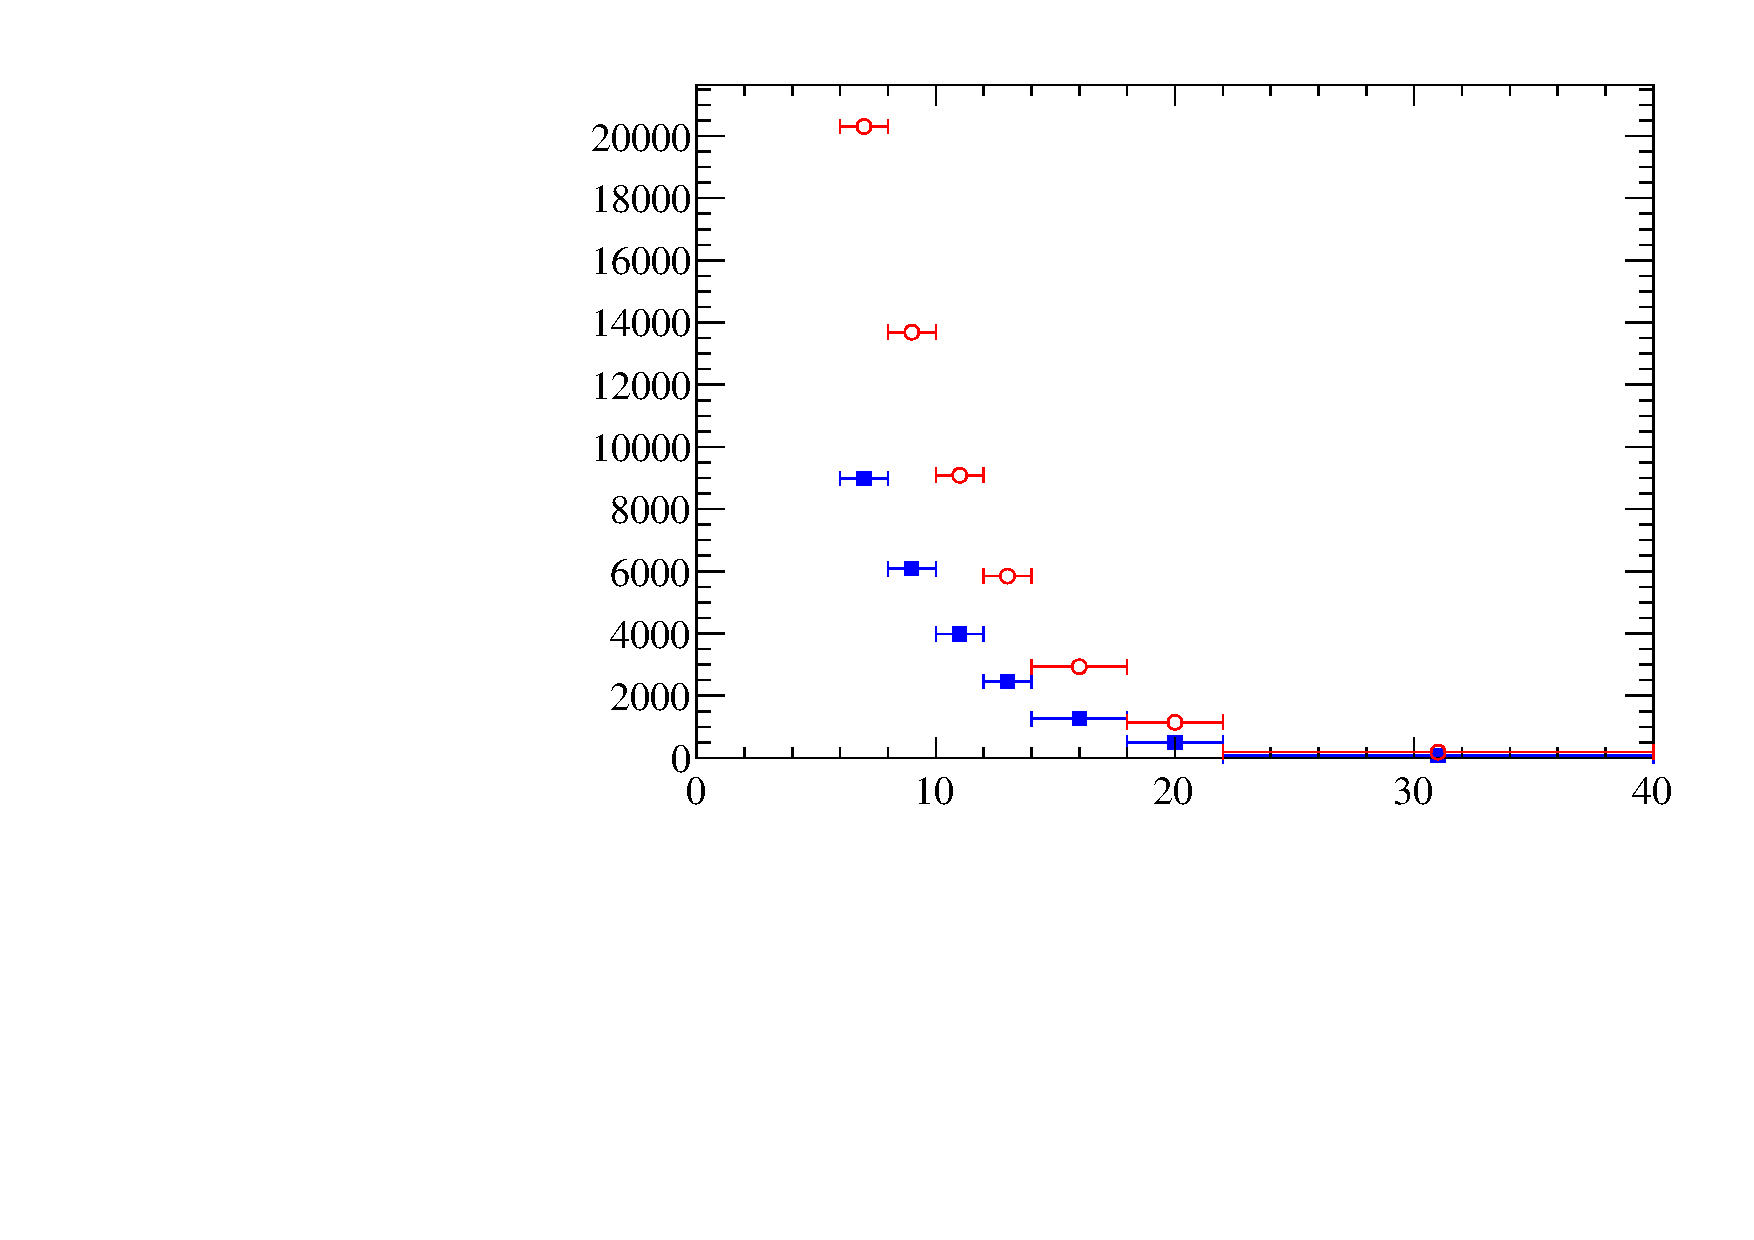
\includegraphics[width=75mm, height=60mm]{upsilon-yields/nups3s}
    }
    \put(0,60){
      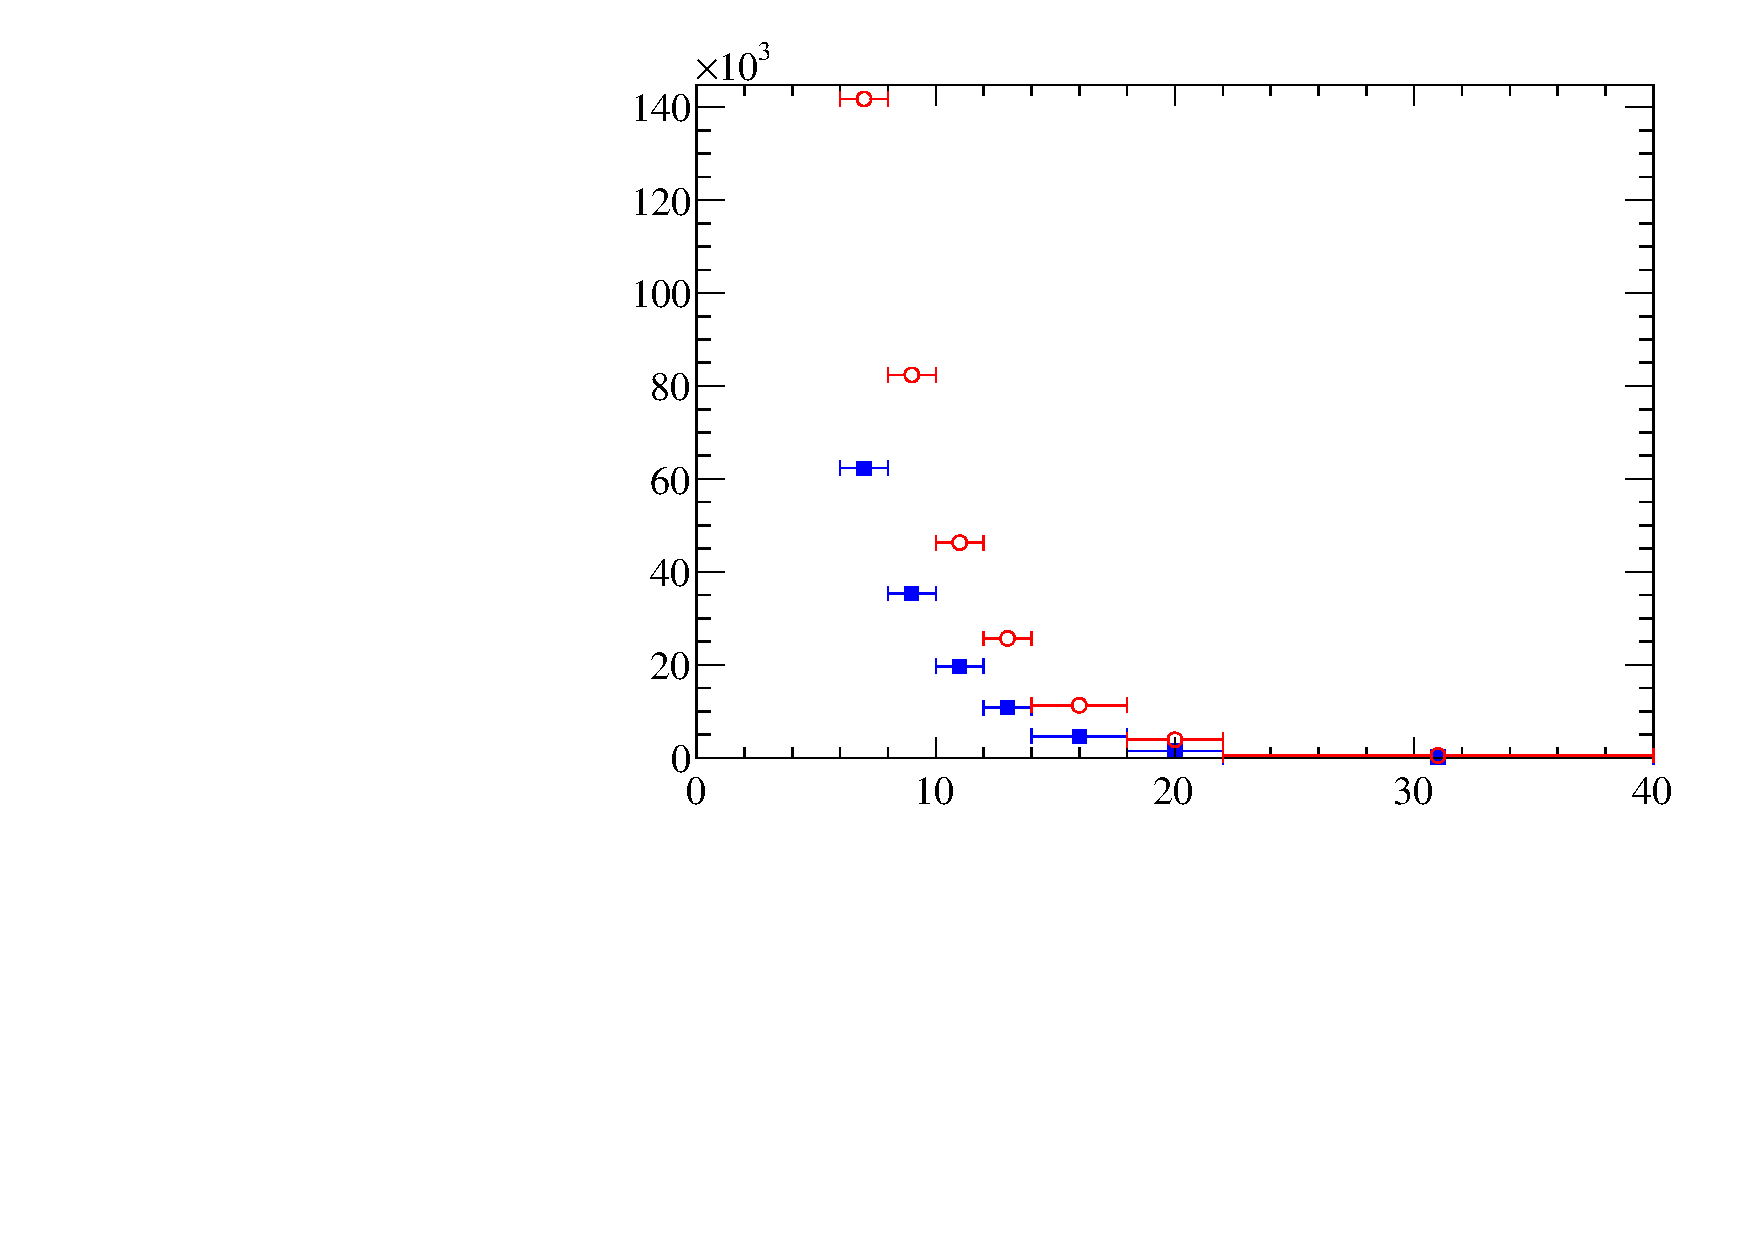
\includegraphics[width=75mm, height=60mm]{upsilon-yields/nups1s}
    }
    \put(75,60){
      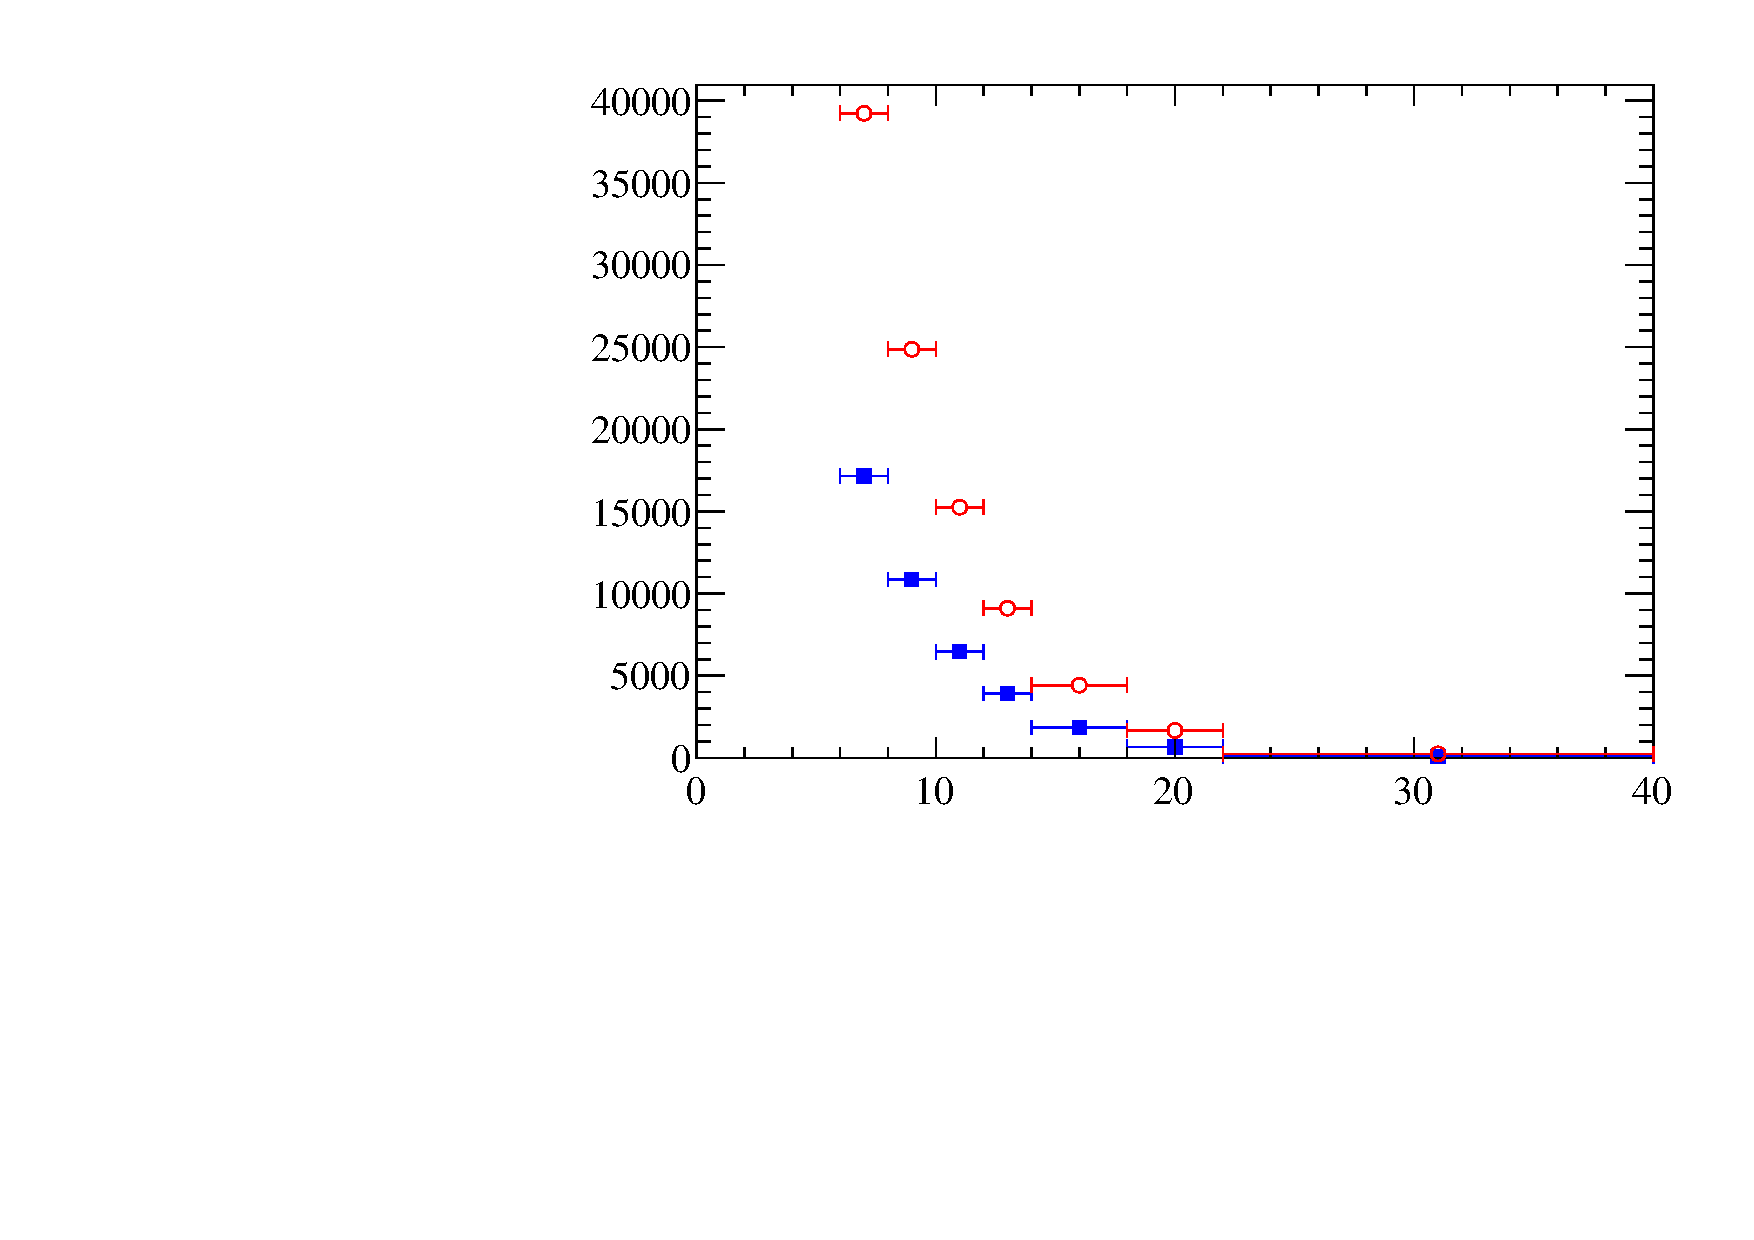
\includegraphics[width=75mm, height=60mm]{upsilon-yields/nups2s}
    }

    \put(2,25){\begin{sideways}Events\end{sideways}}
    \put(35,2){$p_T(\Upsilon) \left[\gevc\right]$}
    \put(55,50){$\Y3S$}

    \put(2,85){\begin{sideways}Events\end{sideways}}
    \put(35,62){$p_T(\Upsilon) \left[\gevc\right]$}
    \put(55,110){$\Y1S$}

    \put(77,85){\begin{sideways}Events\end{sideways}}
    \put(110,62){$p_T(\Upsilon) \left[\gevc\right]$}
    \put(130,110){$\Y2S$}


    \put(50,45){\textcolor{blue}{\sqs=7\tev}}
    \put(50,40){\textcolor{red}{\sqs=8\tev}}
    \put(45,45){
      
\includegraphics[width=3mm, height=2mm]{bsf}
    }
    \put(45,40){
      
\includegraphics[width=3mm, height=2mm]{rco}
    }

    \put(50,105){\textcolor{blue}{\sqs=7\tev}}
    \put(50,100){\textcolor{red}{\sqs=8\tev}}
    \put(45,105){
      
\includegraphics[width=3mm, height=2mm]{bsf}
    }
    \put(45,100){
      
\includegraphics[width=3mm, height=2mm]{rco}
    }

    \put(125,105){\textcolor{blue}{\sqs=7\tev}}
    \put(125,100){\textcolor{red}{\sqs=8\tev}}
    \put(120,105){
      
\includegraphics[width=3mm, height=2mm]{bsf}
    }
    \put(120,100){
      
\includegraphics[width=3mm, height=2mm]{rco}
    }


  % \graphpaper[5](0,0)(75, 60)
  \end{picture}
  }

Yields normalized by bin width.

\begin{block}{}
As expected, yields for 2012 are twice larger than for 2011 due to luminosity difference.
\end{block}
 
\end{frame}



\begin{frame}{\chib selection}
\begin{itemize}
\item In this study photons reconstructed using the calorimeter information. Another approach is to 
track $e^{+}e^{-}$ (converted photons) --- this method has better invariant mass resolution, but requires more statistics.

\item Cuts on $\gamma$:
\begin{center}
\scalebox{0.9}{
\begin{tabular}{lr}\toprule
Transverse momentum of $\gamma$ & $p_T(\gamma) > 600 \mevc$ \\
Polar angle of $\gamma$ in the $\mumu\gamma$ rest frame & $\cos\theta_{\gamma} > 0$ \\
Confidence level of $\gamma$ & $cl(\gamma) > 0.01$ \\
\bottomrule
\end{tabular}
}
\end{center}

\bigskip

\item Dimuon mass windows:
\begin{center}
\scalebox{0.6}{
\begin{tabular}{lrr}\toprule
\multicolumn{1}{c}{Decay} & \multicolumn{1}{c}{Cut} & \multicolumn{1}{c}{Description}\\
\midrule
$\chib(1,2,3P) \to \Upsilon(1S)$ & $9310 < \mumu < 9600 \mevc$ & $3 \sigma_{\Y1S} < \mumu < 2.5 \sigma_{\Y1S} \mevc$\\
$\chib(2,3P) \to \Upsilon(2S)$ & $9870 < \mumu < 10090  \mevc$ &  $3 \sigma_{\Y2S} < \mumu < \sigma_{\Y2S} \mevc$\\
$\chib(3P) \to \Upsilon(3S)$ & $10300 < \mumu < 10526  \mevc$ &   $\sigma_{\Y3S} < \mumu < 3 \sigma_{\Y3S} \mevc$\\
\bottomrule
\end{tabular}
}
\end{center}

\end{itemize}
\end{frame}

\begin{frame}{$\chi_{b1,2}(1,2,3P) \to \OneS$ fit model}
\begin{columns}
\column{.5\textwidth}
  \centering
  \setlength{\unitlength}{1mm}
  \begin{picture}(50,80)
      %
    \put(0,0){
      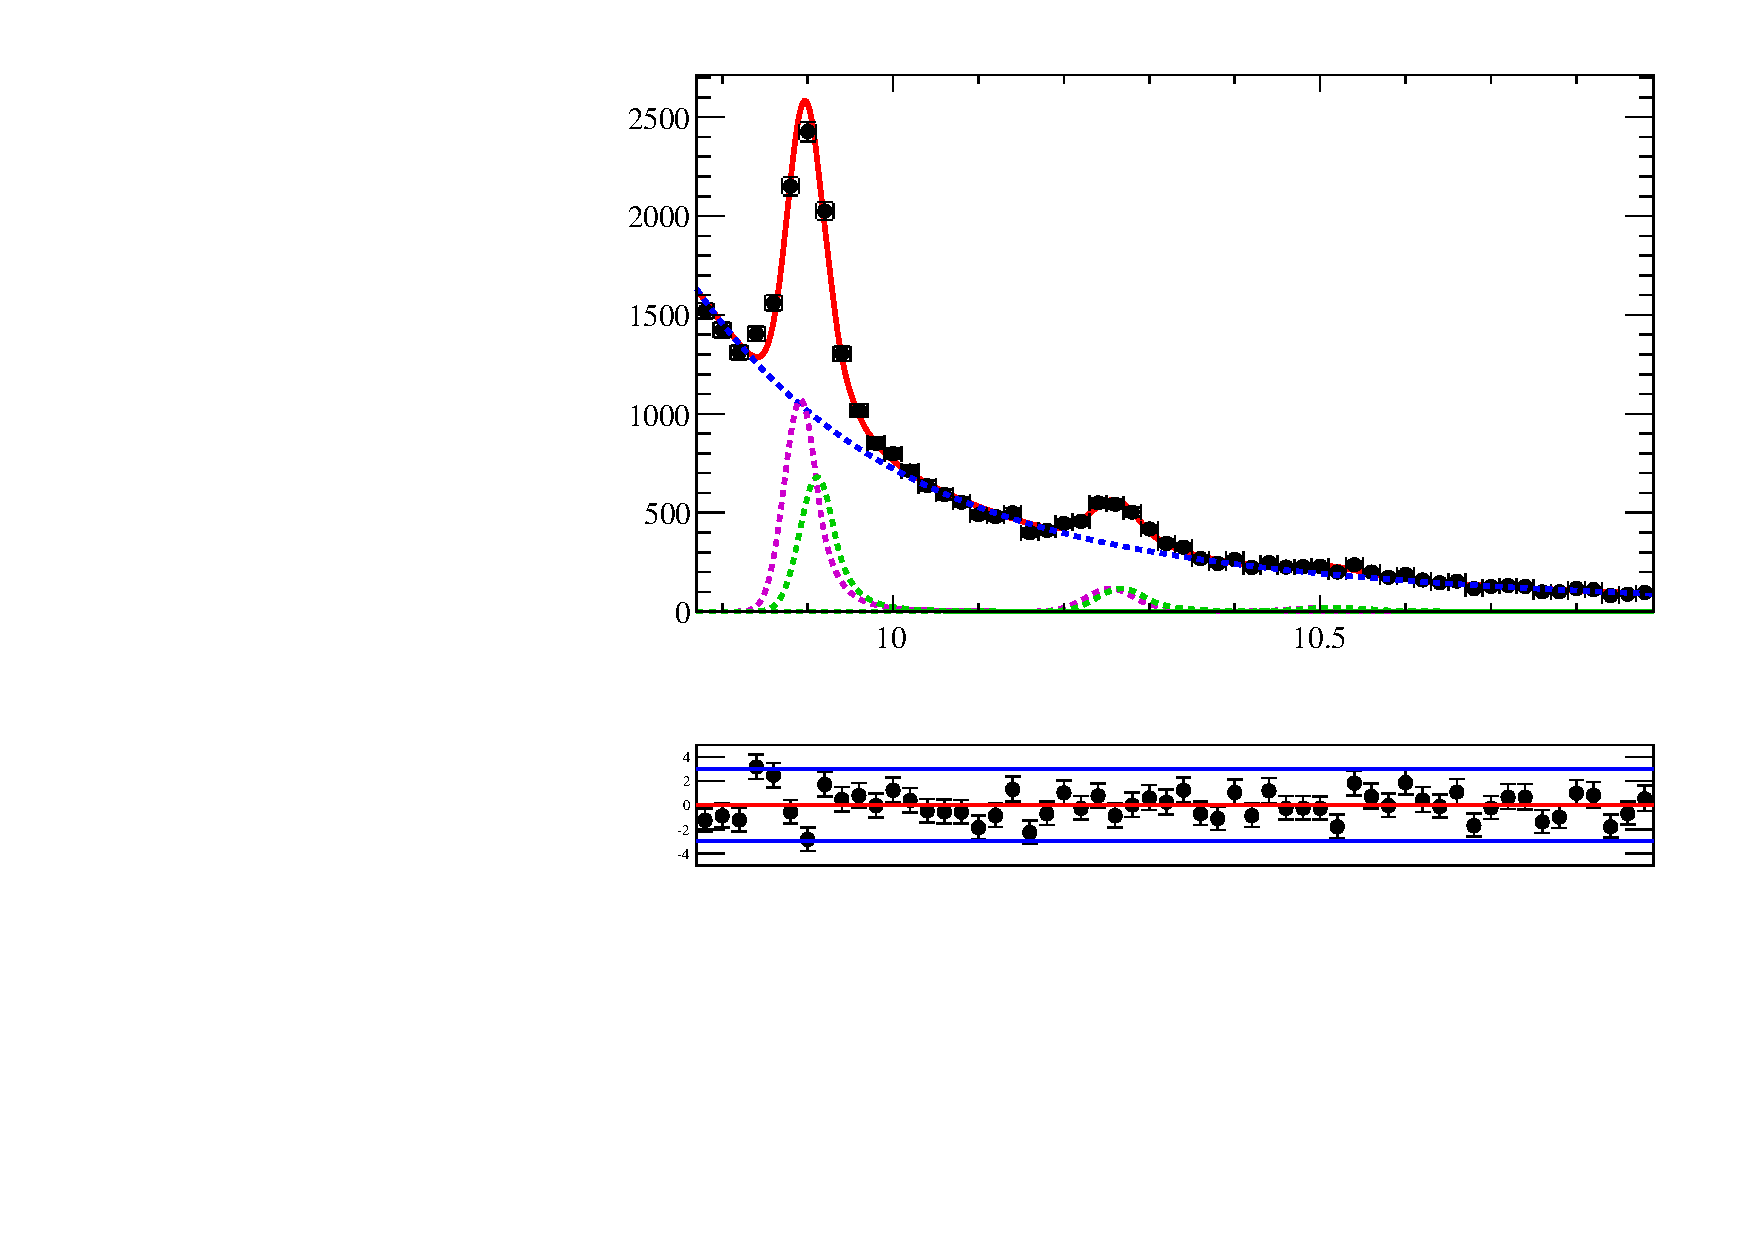
\includegraphics[width=50mm, height=40mm]{chib1s-fit/f2012_fix_14_None}
    }
    
    \put(0,40){
      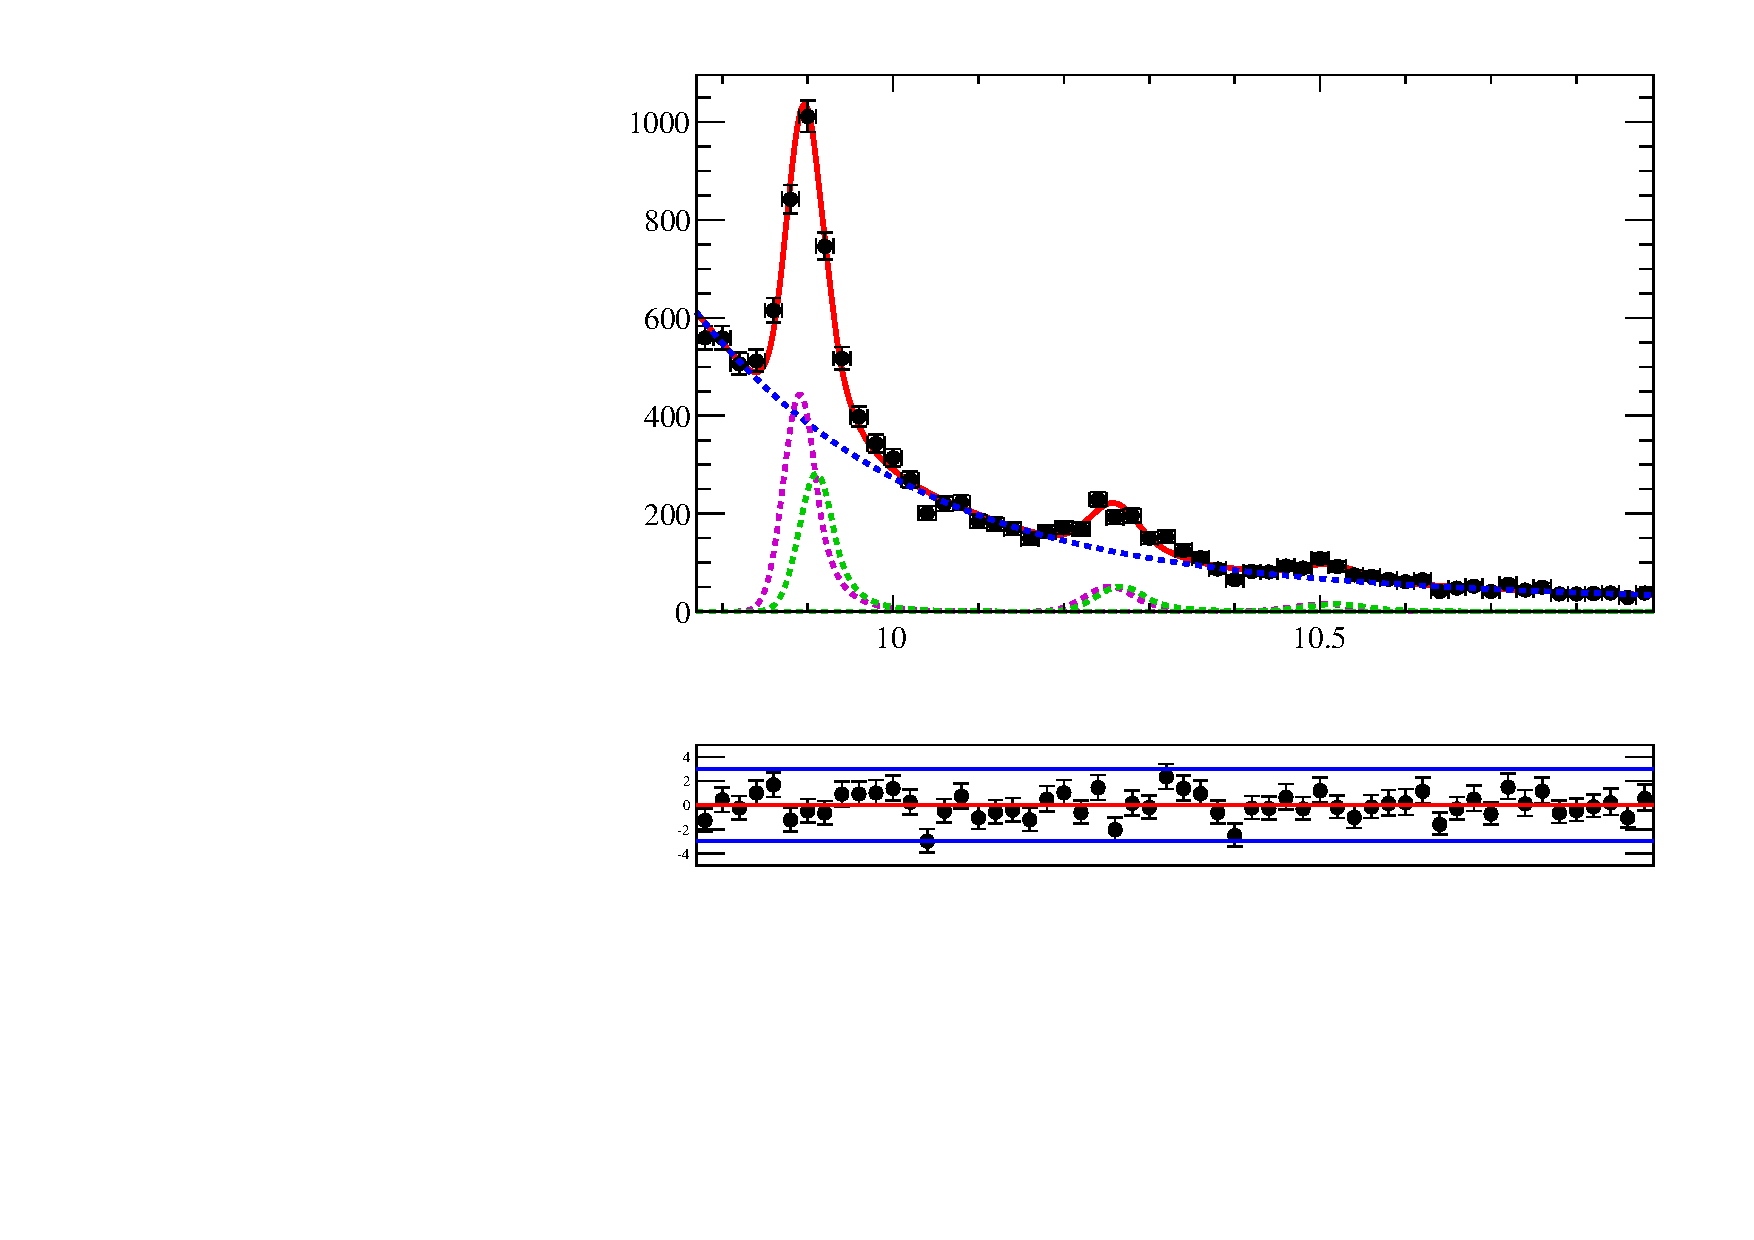
\includegraphics[width=50mm, height=40mm]{chib1s-fit/f2011_fix_14_None}
    }

    \put(0,15){\tiny \begin{sideways}Candidates/(20\mevcc)\end{sideways}}
    \put(5,9.5){\tiny $m_{\mumu \gamma} - m_{\mumu} + 9.4603 \left[\gevcc\right]$}
    \put(25,30){$\sqrt{s} = 8 \tev$}
    \put(20,25){\tiny $p_T(\Y1S) > 14 \gevc$}
    
    \put(0,55){\tiny \begin{sideways}Candidates/(20\mevcc)\end{sideways}}
    \put(5, 49.5){\tiny $m_{\mumu \gamma} - m_{\mumu} + 9.4603 \left[\gevcc\right]$}
    \put(25,70){$\sqrt{s} = 7 \tev$}
    \put(20,65){\tiny $p_T(\Y1S) > 14 \gevc$}
    %\graphpaper[2](0,0)(50, 40)        
  \end{picture}
\column{.5\textwidth}
\begin{itemize}
\item 6 Crystal Ball functions for each of $\chi_{b1,2}(1,2,3P)$ signal (exclude
the study of $\chi_{b0}$ due to its low branching ratio)
\item Product of exponential and linear combination of basic Bernstein
polinomials  for combinatorial background.
\end{itemize}
\end{columns}
\end{frame}

\begin{frame}{$\chi_{b1,2}(1,2,3P) \to \OneS$ fit model (2)}
\begin{columns}[T]
\column{.6\textwidth}
\begin{itemize}
\item Free parameters: $\mu_{\chi_{b1}(1P)}$, yields and background parameters.
\item Linked parameters for \chibone and \chibtwo signals:
    \begin{itemize}
    \item $\mu_{\chi_{b2}(jP)} = \mu_{\chi_{b1}(jP)} + \Delta m_{\chi_{b2}(jP)}^{PDG}$, j=1,2
    \item $\mu_{\chi_{b2}(3P)} = \mu_{\chi_{b1}(3P)} + \Delta m_{\chi_{b2}(3P)}^{theory}$
    \item $N_{\chi_{b}} = \lambda N_{\chi_{b1}} + (1-\lambda) N_{\chi_{b2}}$
    \item $\sigma_{\chi_{b2}} = \sigma_{\chi_{b1}}$
    \end{itemize}
\item Other linked parameters:    
    \begin{itemize}
        \item $\mu_{\chiboneTwoP} = \mu_{\chiboneOneP} + \Delta m_{\chi_{b1}(2P)}^{PDG}$
        \item $\mu_{\chiboneThreeP} = \mu_{\chiboneOneP} + \Delta m_{\chi_{b1}(3P)}$ ($\Delta m_{\chi_{b1}(3P)}$ measured in this study)
    \end{itemize}
\item Fixed parameters from MC study:
    \begin{itemize}
    \item $\sigma_{\chiboneOneP}$ \scriptsize{scaled by 1.17}, $\frac{\sigma_{\chiboneTwoP}}{\sigma_{\chiboneOneP}}$,$\frac{\sigma_{\chiboneThreeP}}{\sigma_{\chiboneOneP}}$
    \item $\alpha$ and $n$ parameters of CB.
    \end{itemize}
\end{itemize}
\column{.4\textwidth}
\scalebox{0.34}{
    \begin{tabular}{lrrr}\toprule
    & \multicolumn{ 3 }{c}{\OneS transverse momentum intervals} \\
     & & \multicolumn{2}{c}{$p_T(\Upsilon)> 14 \gevc$} \\
    \cmidrule{3-4}
     && \sqs = 7 \tev & \sqs = 8\tev \\
    \midrule
    $N_{\chi_{b}(1P)}$  && 1960 $\pm$ 70 & 4730 $\pm$ 120 \\
    $N_{\chi_{b}(2P)}$  && 410 $\pm$ 40 & 930 $\pm$ 70 \\
    $N_{\chi_{b}(3P)}$  && 154 $\pm$ 34 & 220 $\pm$ 50 \\
    \rule{0pt}{4ex}$B$  && 9230 $\pm$ 120 & 24,870 $\pm$ 200 \\
    \rule{0pt}{4ex}$\mu_{\chi_{b1}(1P)}, \mevcc$  && 9890.9 $\pm$ 1.0 & 9891.6 $\pm$ 0.7 \\

    $\Delta m_{\chiboneTwoP}, \mevcc$  && \multicolumn{2}{c}{363} \\
    $\Delta m_{\chiboneThreeP}, \mevcc$  && \multicolumn{2}{c}{614} \\

    \rule{0pt}{4ex}$\Delta m_{\chi_{b2,1}(1P)}^{PDG}, \mevcc$  && \multicolumn{2}{c}{19.43} \\
    $\Delta m_{\chi_{b2,1}(2P)}^{PDG}, \mevcc$  && \multicolumn{2}{c}{13.19} \\
    $\Delta m_{\chi_{b2,1}(2P)}^{theory}, \mevcc$  && \multicolumn{2}{c}{13.00} \\

    \rule{0pt}{4ex}$\sigma_{\chi_{b1}(1P)}, \mevcc$  && \multicolumn{2}{c}{19.02} \\
    $\sigma_{\chi_{b2}(1P)}/\sigma_{\chi_{b1}(1P)}, \mevcc$  && \multicolumn{2}{c}{1.05} \\
    $\sigma_{\chi_{b1}(2P)} / \sigma_{\chi_{b1}(1P)}, \mevcc$  && \multicolumn{2}{c}{1.50} \\
    $\sigma_{\chi_{b1}(3P)} / \sigma_{\chi_{b1}(1P)}, \mevcc$  && \multicolumn{2}{c}{2.00} \\

    \rule{0pt}{4ex}$\lambda_{\chibOneP}$  && \multicolumn{2}{c}{0.6} \\
    $\lambda_{\chibTwoP}$  && \multicolumn{2}{c}{0.5} \\
    $\lambda_{\chibThreeP}$  && \multicolumn{2}{c}{0.5} \\

    \rule{0pt}{4ex}$\alpha_{\chi_{b}(1P)}$  && \multicolumn{2}{c}{-1.10} \\
    $\alpha_{\chi_{b}(2P)}$  && \multicolumn{2}{c}{-1.10} \\
    $\alpha_{\chi_{b}(3P)}$  && \multicolumn{2}{c}{-1.25} \\

    \rule{0pt}{4ex}$n_{\chi_{b}(1P)}$  && \multicolumn{2}{c}{5.0} \\
    $n_{\chi_{b}(2P)}$  && \multicolumn{2}{c}{5.0} \\
    $n_{\chi_{b}(3P)}$  && \multicolumn{2}{c}{5.0} \\

    \rule{0pt}{4ex}$\tau$  && -2.5 $\pm$ 0.5 & -3.02 $\pm$ 0.30 \\
    $c_0$  && -0.10 $\pm$ 0.11 & 0.02 $\pm$ 0.06 \\
    $c_1$  && 1.36 $\pm$ 0.04 & 0.25 $\pm$ 0.04 \\


    \rule{0pt}{4ex}$\chi^2 / n.d.f$  && 1.2 & 1.5 \\
    \bottomrule
\end{tabular}
}

\bigskip
{\tiny \textcolor{blue}{Good agreement between $\mu_{\chi_{b1}(1P)}$ and value  in PDG (9892 \mevcc).}}
\end{columns}


\end{frame}

\begin{frame}{Mass of \chiboneOneP in $\chib \to \OneS \gamma$ decay}
\setlength{\unitlength}{1mm}
\begin{picture}(70,50)
  %
\put(0,0){
  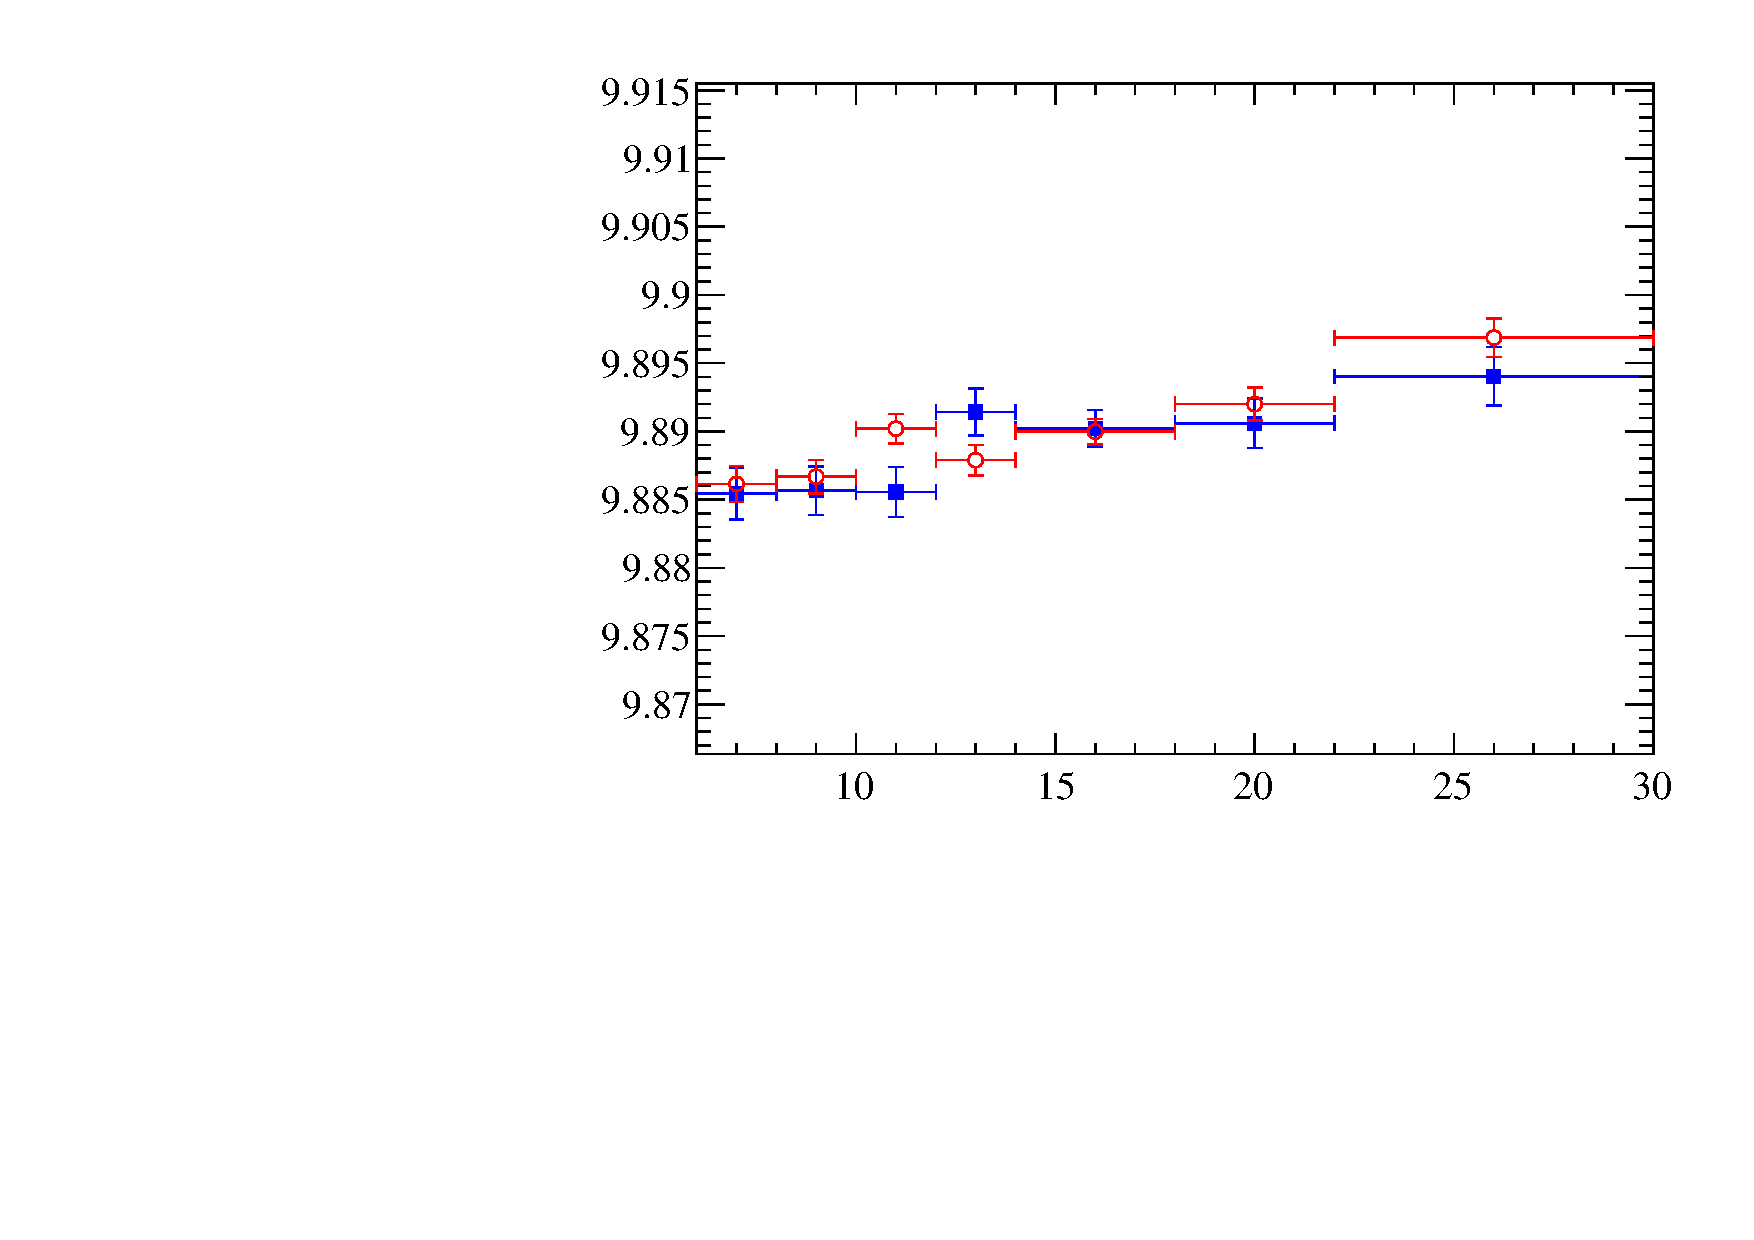
\includegraphics[width=70mm, height=50mm]{chib1s-m/mass1p}
}

\put(27, 40){\textcolor{blue}{\sqs=7\tev}, \textcolor{red}{\sqs=8\tev}}
\put(27, 40){\textcolor{blue}{\sqs=7\tev}, \textcolor{red}{\sqs=8\tev}}
\put(0,12){\begin{sideways}\chiboneOneP mass \gevcc\end{sideways}}
\put(20,1){$p_T(\Upsilon) \left[\gevc\right]$}
\end{picture}

\begin{alertblock}{}
The major cause of  \chiboneOneP mass floating in 10 \mevc range can be the unknown fraction
between $N_{\chibone}$ and $N_{\chibtwo}$ yields ($\lambda$ parameter). 
We have only theoretical prediction for $\lambda$ value .
\end{alertblock}

In this study the mass of \chiboneOneP was fixed to \textcolor{blue}{9892} \mevcc.

\end{frame}
\begin{frame}{$\chi_b$ yields in $\chi_b \to \OneS$ decays}
\scalebox{0.8}{
  \setlength{\unitlength}{1mm}
  \centering
  \scalebox{0.7}{
  \begin{picture}(150,120)
    \put(0,0){
      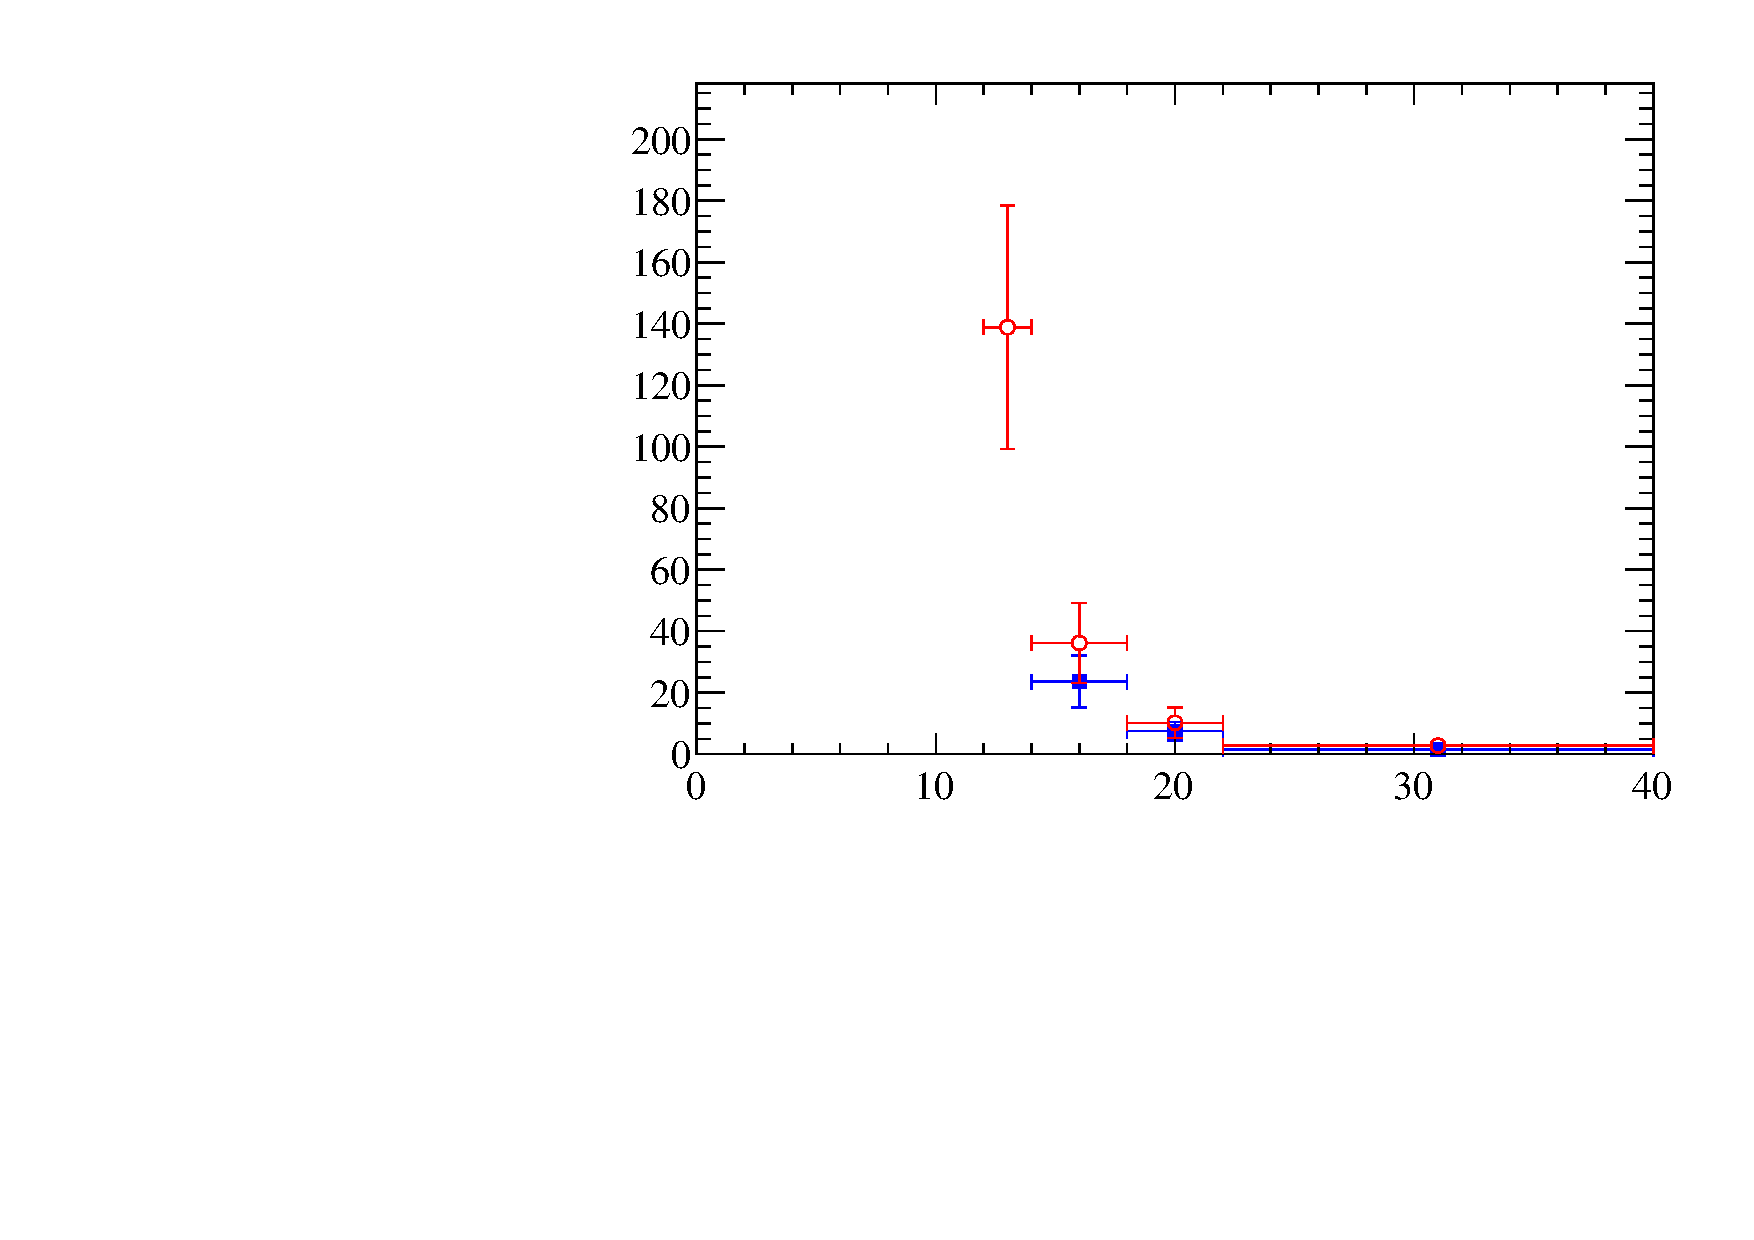
\includegraphics[width=75mm, height=60mm]{chib1s-yields/n3p_1s}
    }
    \put(0,60){
      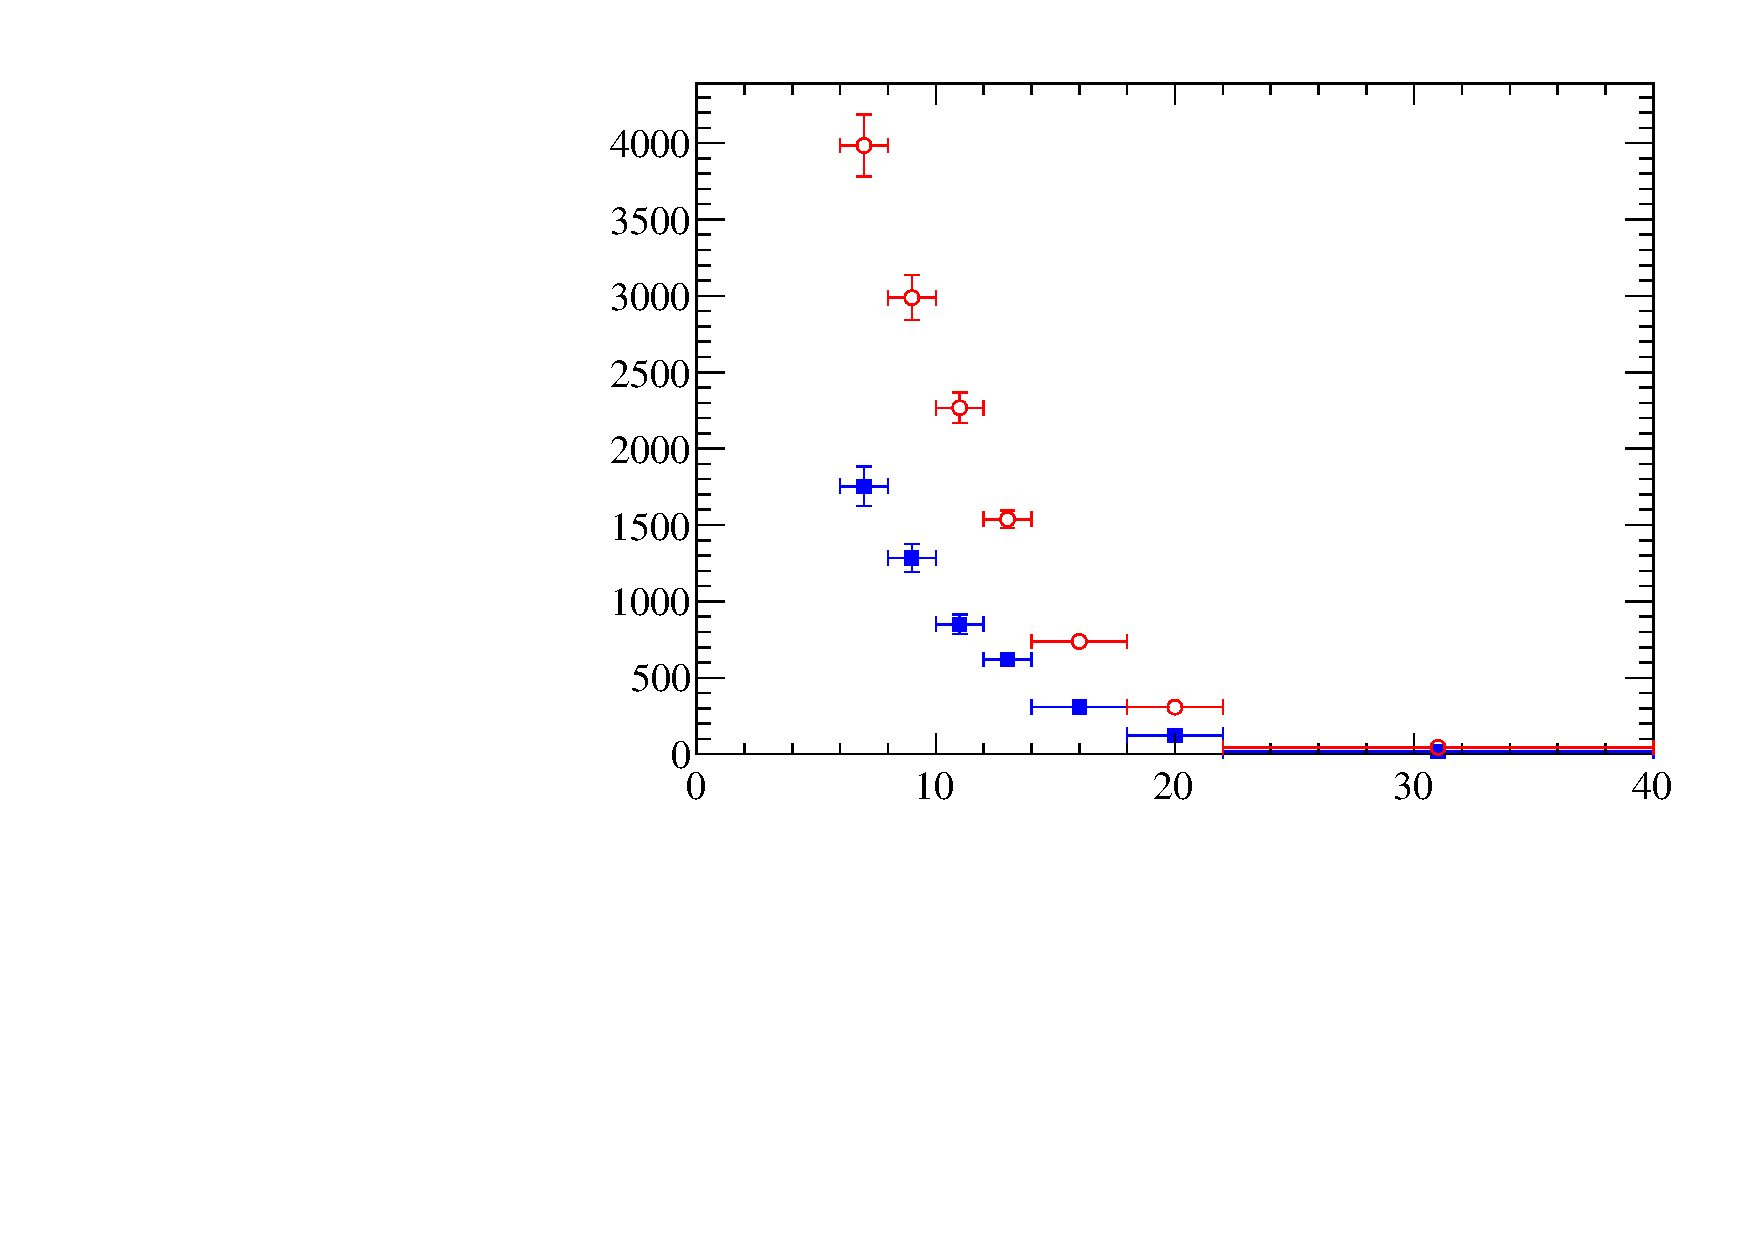
\includegraphics[width=75mm, height=60mm]{chib1s-yields/n1p_1s}
    }
    \put(75,60){
      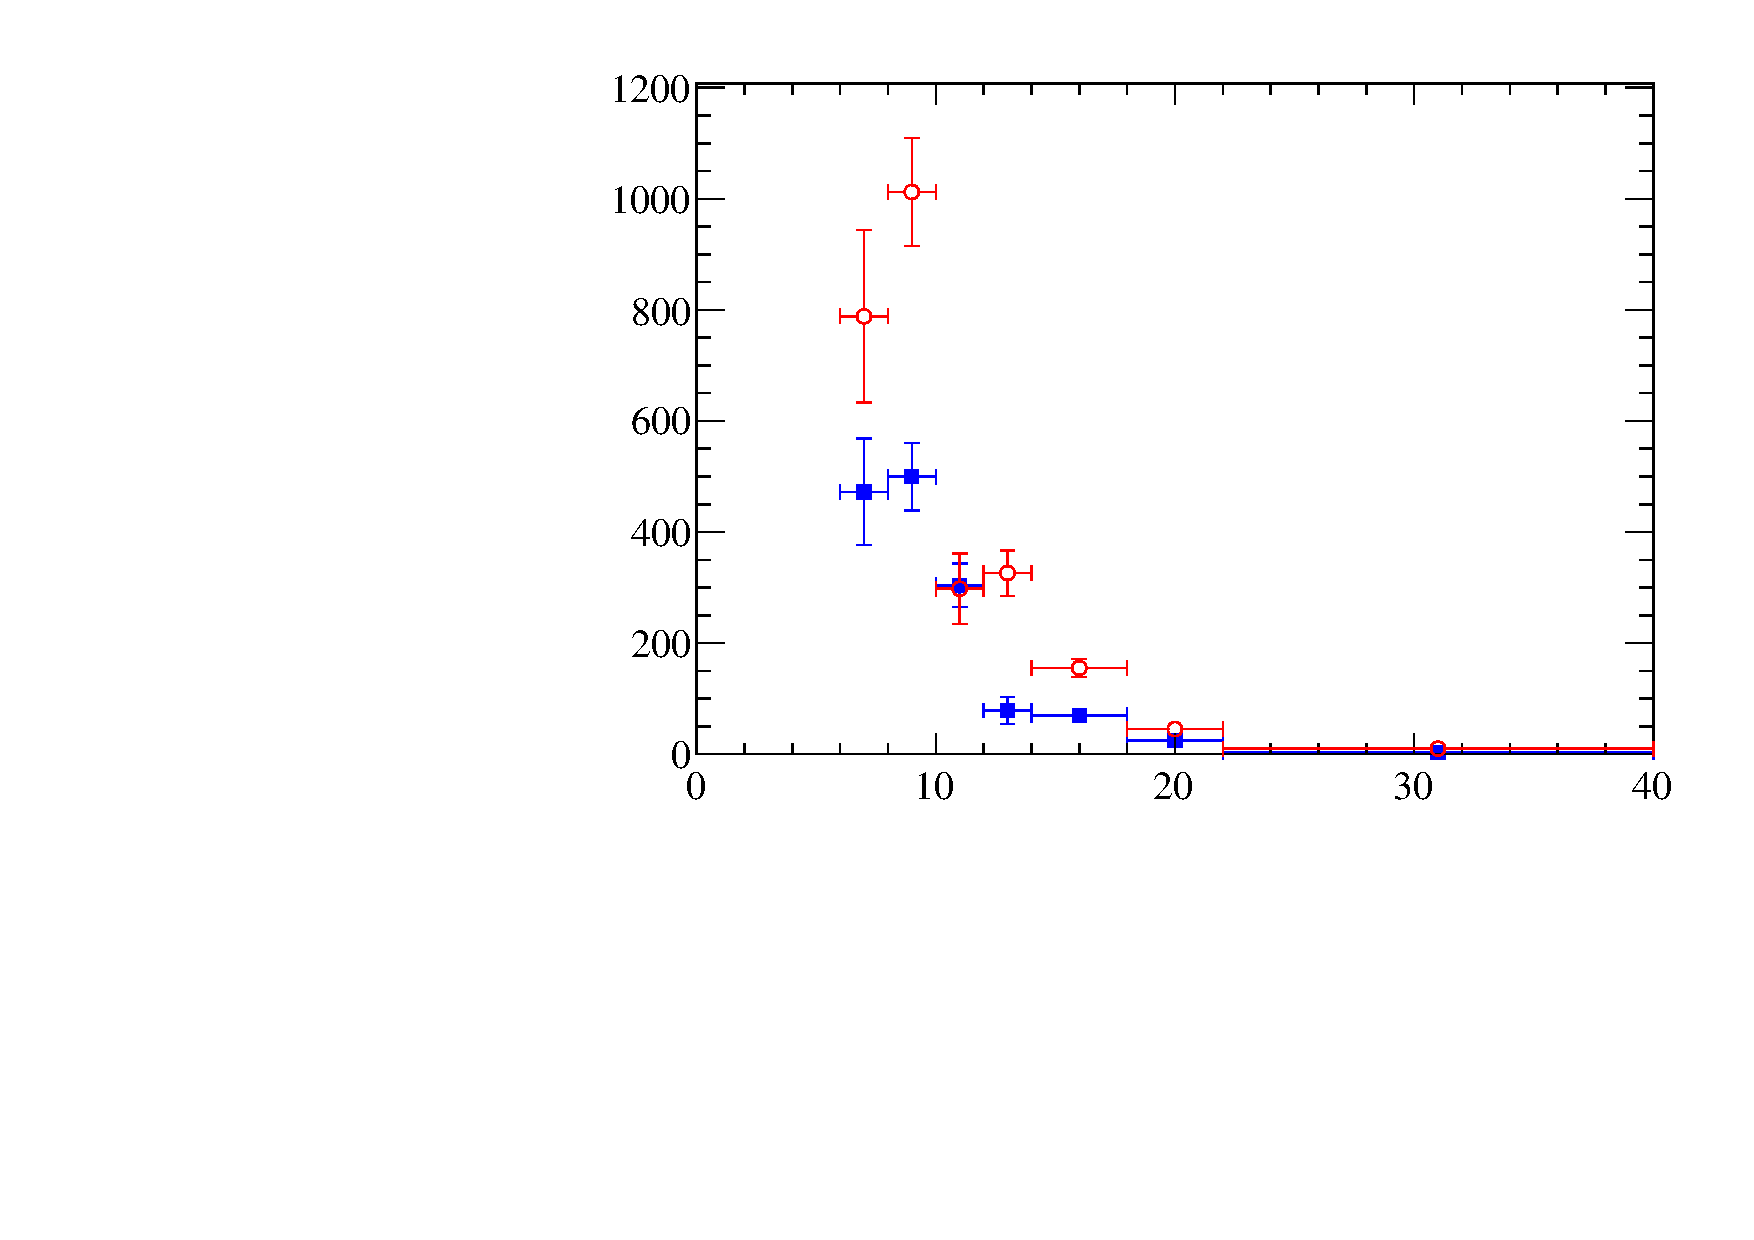
\includegraphics[width=75mm, height=60mm]{chib1s-yields/n2p_1s}
    }

    \put(2,25){\begin{sideways}Events\end{sideways}}
    \put(35,2){$p_T^{\Y1S} \left[\gevc\right]$}
    \put(55,50){$\chibThreeP$}

    \put(2,85){\begin{sideways}Events\end{sideways}}
    \put(35,62){$p_T^{\Y1S} \left[\gevc\right]$}
    \put(55,110){$\chibOneP$}

    \put(77,85){\begin{sideways}Events\end{sideways}}
    \put(110,62){$p_T^{\Y1S} \left[\gevc\right]$}
    \put(130,110){$\chibTwoP$}


    \put(50,45){\textcolor{blue}{\sqs=7\tev}}
    \put(50,40){\textcolor{red}{\sqs=8\tev}}
    \put(45,45){
      
\includegraphics[width=3mm, height=2mm]{bsf}
    }
    \put(45,40){
      
\includegraphics[width=3mm, height=2mm]{rco}
    }

    \put(50,105){\textcolor{blue}{\sqs=7\tev}}
    \put(50,100){\textcolor{red}{\sqs=8\tev}}
    \put(45,105){
      
\includegraphics[width=3mm, height=2mm]{bsf}
    }
    \put(45,100){
      
\includegraphics[width=3mm, height=2mm]{rco}
    }

    \put(125,105){\textcolor{blue}{\sqs=7\tev}}
    \put(125,100){\textcolor{red}{\sqs=8\tev}}
    \put(120,105){
      
\includegraphics[width=3mm, height=2mm]{bsf}
    }
    \put(120,100){
      
\includegraphics[width=3mm, height=2mm]{rco}
   }
  % \graphpaper[5](0,0)(75, 60)
  \end{picture}
}  
}
\begin{center}
Yields normalized by bin width.
\end{center}  
\end{frame}


\begin{frame}{$\chi_{b1,2}(2,3P) \to \TwoS$ fit model}
\begin{columns}[T]
\column{.5\textwidth}
  \centering
  \setlength{\unitlength}{1mm}
  \begin{picture}(50,80)
      %
    \put(0,0){
      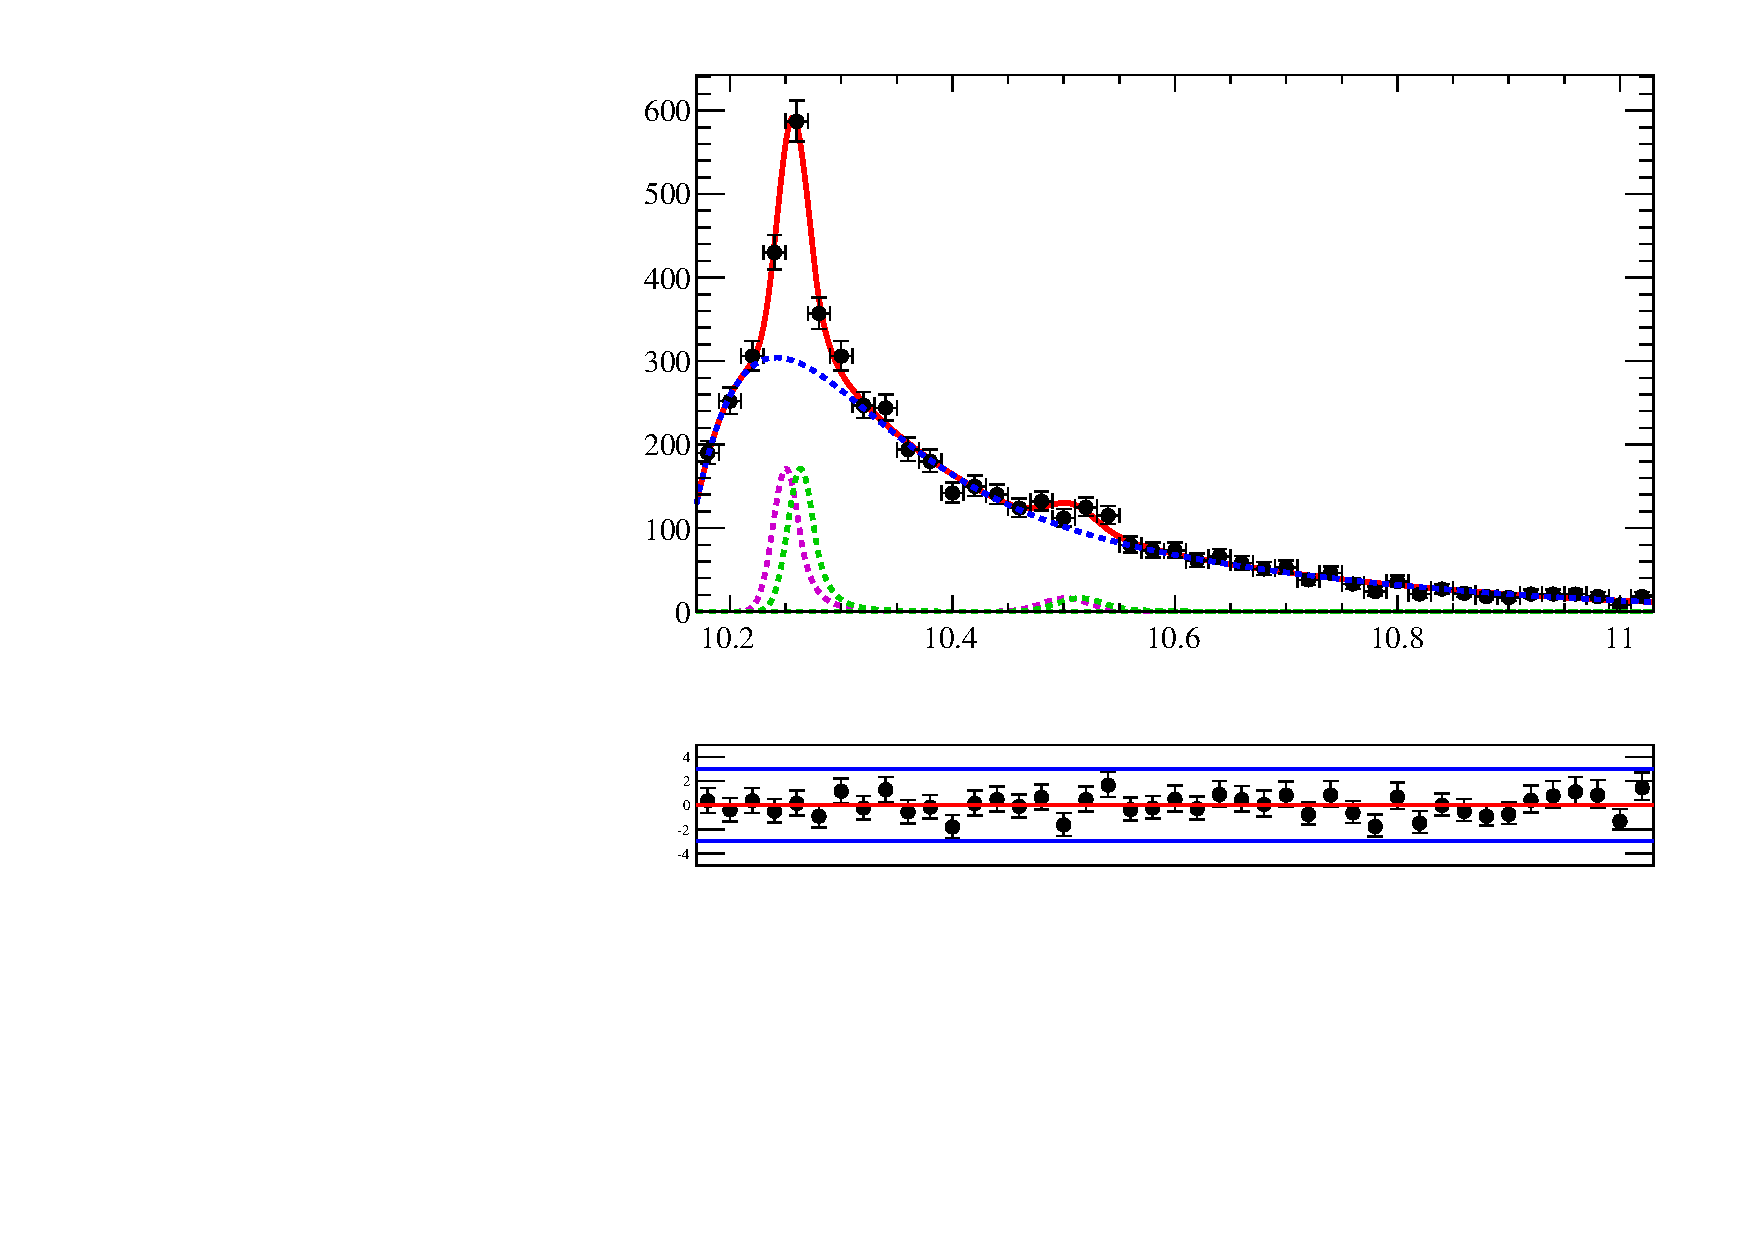
\includegraphics[width=50mm, height=40mm]{chib2s-fit/f2012_fix_18_None}
    }
    
    \put(0,40){
      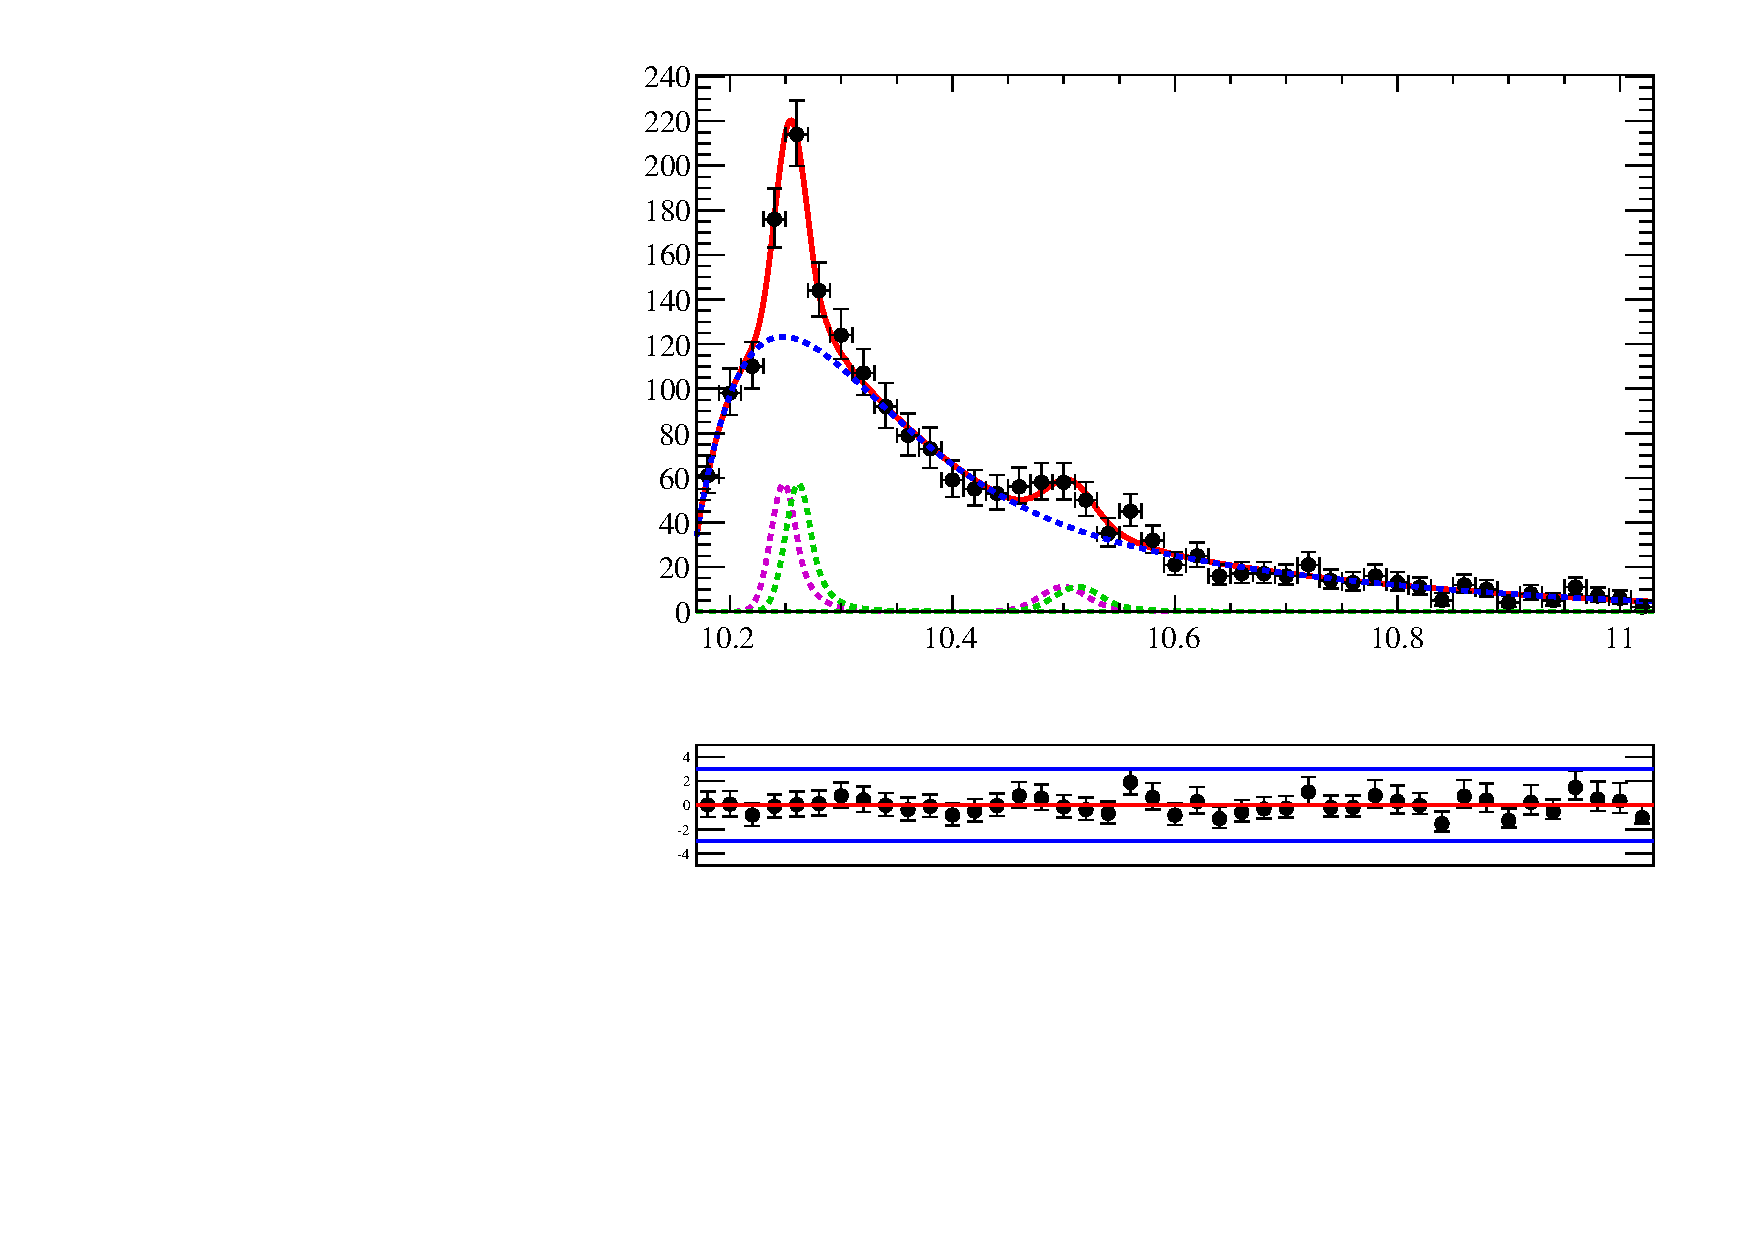
\includegraphics[width=50mm, height=40mm]{chib2s-fit/f2011_fix_18_None}
    }

    \put(0,15){\tiny \begin{sideways}Candidates/(20\mevcc)\end{sideways}}
    \put(2,9.5){\tiny $m_{\mumu \gamma} - m_{\mumu} + 10.02326 \left[\gevcc\right]$}
    \put(25,30){$\sqrt{s} = 8 \tev$}
    \put(20,25){\tiny $p_T(\Y2S) > 18 \gevc$}
    
    \put(0,55){\tiny \begin{sideways}Candidates/(20\mevcc)\end{sideways}}
    \put(2, 49.5){\tiny $m_{\mumu \gamma} - m_{\mumu} + 10.02326 \left[\gevcc\right]$}
    \put(25,70){$\sqrt{s} = 7 \tev$}
    \put(20,65){\tiny $p_T(\Y2S) > 18 \gevc$}
    %\graphpaper[2](0,0)(50, 40)        
  \end{picture}
\column{.5\textwidth}
\begin{itemize}
\item 4 Crystal Ball function for each of $\chi_{b1,2}(2,3P)$ signal
\item Product of exponential and linear combination of basic Bernstein polinomials  for combinatorial background.
\end{itemize}
\end{columns}
\end{frame}

\begin{frame}{$\chi_{b1,2}(2,3P) \to \TwoS$ fit model (2)}
\begin{columns}[T]
\column{.6\textwidth}
\begin{itemize}
\item Free parameters: $\mu_{\chi_{b1}(2P)}$, yields and background parameters.
\item Linked parameters for \chibone and \chibtwo signals:
    \begin{itemize}
    \item $\mu_{\chi_{b2}(2P)} = \mu_{\chi_{b1}(2P)} + \Delta m_{\chi_{b2}(2P)}^{PDG}$
    \item $\mu_{\chi_{b2}(3P)} = \mu_{\chi_{b1}(3P)} + \Delta m_{\chi_{b2}(3P)}^{theory}$
    \item $N_{\chi_{b}} = \lambda N_{\chi_{b1}} + (1-\lambda) N_{\chi_{b2}}$
    \item $\sigma_{\chi_{b2}} = \sigma_{\chi_{b1}}$
    \end{itemize}
\item Other linked parameters:    
    \begin{itemize}
        \item $\mu_{\chiboneThreeP} = \mu_{\chiboneOneP} + \Delta m_{\chi_{b1}(3P)}$ ($\Delta m_{\chi_{b1}(3P)}$ measured in this study)
    \end{itemize}
\item Fixed parameters from MC study:
    \begin{itemize}
    \item $\sigma_{\chiboneTwoP}$,  $\frac{\sigma_{\chiboneThreeP}}{\sigma_{\chiboneTwoP}}$
    \item $\alpha$ and $n$ parameters of CB.
    \end{itemize}
\end{itemize}
\column{.4\textwidth}
\scalebox{0.34}{
    \begin{tabular}{lrrr}\toprule
    & \multicolumn{ 3 }{c}{\TwoS transverse momentum intervals} \\
     & & \multicolumn{2}{c}{$p_T(\Y2S)> 18 \gevc$} \\
    \cmidrule{3-4}
     && \sqs = 7 \tev & \sqs = 8\tev \\
    \midrule
    $N_{\chi_{b}(2P)}$  && 185 $\pm$ 30 & 550 $\pm$ 50 \\
    $N_{\chi_{b}(3P)}$  && 64 $\pm$ 19 & 93 $\pm$ 29 \\
    \rule{0pt}{4ex}$B$  && 1800 $\pm$ 50 & 4590 $\pm$ 80 \\
    \rule{0pt}{4ex}$\mu_{\chi_{b1}(2P)}, \mevcc$  && 10,248.3 $\pm$ 2.3 & 10,250.4 $\pm$ 1.3 \\

    $\Delta m_{\chiboneThreeP}, \mevcc$  && \multicolumn{2}{c}{252} \\
    \rule{0pt}{4ex}$\Delta m_{\chi_{b2,1}(2P)}^{PDG}, \mevcc$  && \multicolumn{2}{c}{13.19} \\
    $\Delta m_{\chi_{b2,1}(3P)}, \mevcc$  && \multicolumn{2}{c}{13.00} \\

    \rule{0pt}{4ex}$\sigma_{\chi_{b1}(2P)}, \mevcc$  && \multicolumn{2}{c}{11.58} \\
    $\sigma_{\chi_{b1}(3P)} / \sigma_{\chi_{b1}(2P)}, \mevcc$  && \multicolumn{2}{c}{1.84} \\

    \rule{0pt}{4ex}$\lambda_{\chibTwoP}$  && \multicolumn{2}{c}{0.5} \\
    $\lambda_{\chibThreeP}$  && \multicolumn{2}{c}{0.5} \\

    \rule{0pt}{4ex}$\alpha_{\chi_{b}(2P)}$  && \multicolumn{2}{c}{-1.10} \\
    $\alpha_{\chi_{b}(3P)}$  && \multicolumn{2}{c}{-1.25} \\

    \rule{0pt}{4ex}$n_{\chi_{b}(2P)}$  && \multicolumn{2}{c}{5.0} \\
    $n_{\chi_{b}(3P)}$  && \multicolumn{2}{c}{5.0} \\

    \rule{0pt}{4ex}$\tau$  && -8.3 $\pm$ 2.9 & -8.6 $\pm$ 1.2 \\
    $c_0$  && 0.40 $\pm$ 0.06 & 0.392 $\pm$ 0.030 \\
    $c_1$  && -2.30 $\pm$ 0.30 & -2.35 $\pm$ 0.10 \\
    $c_2$  && -2.6 $\pm$ 0.6 & -2.67 $\pm$ 0.13 \\
    $c_3$  && 0.3 $\pm$ 0.6 & 0.36 $\pm$ 0.24 \\
    $c_4$  &&  -  &  -  \\

    \rule{0pt}{4ex}$\chi^2 / n.d.f$  && 0.6 & 1.0 \\
    \bottomrule
\end{tabular}
}

\bigskip
{\tiny \textcolor{blue}{The mass of $\chi_{b1}(2P)$  is about 5 \mevcc  less than value in PDG (10.25546 \mevcc).}}
\end{columns}


\end{frame}

\begin{frame}{Mass of \chiboneTwoP in $\chib \to \TwoS \gamma$ decay}
\begin{center}
\setlength{\unitlength}{1mm}
\begin{picture}(70,50)
  %
\put(0,0){
  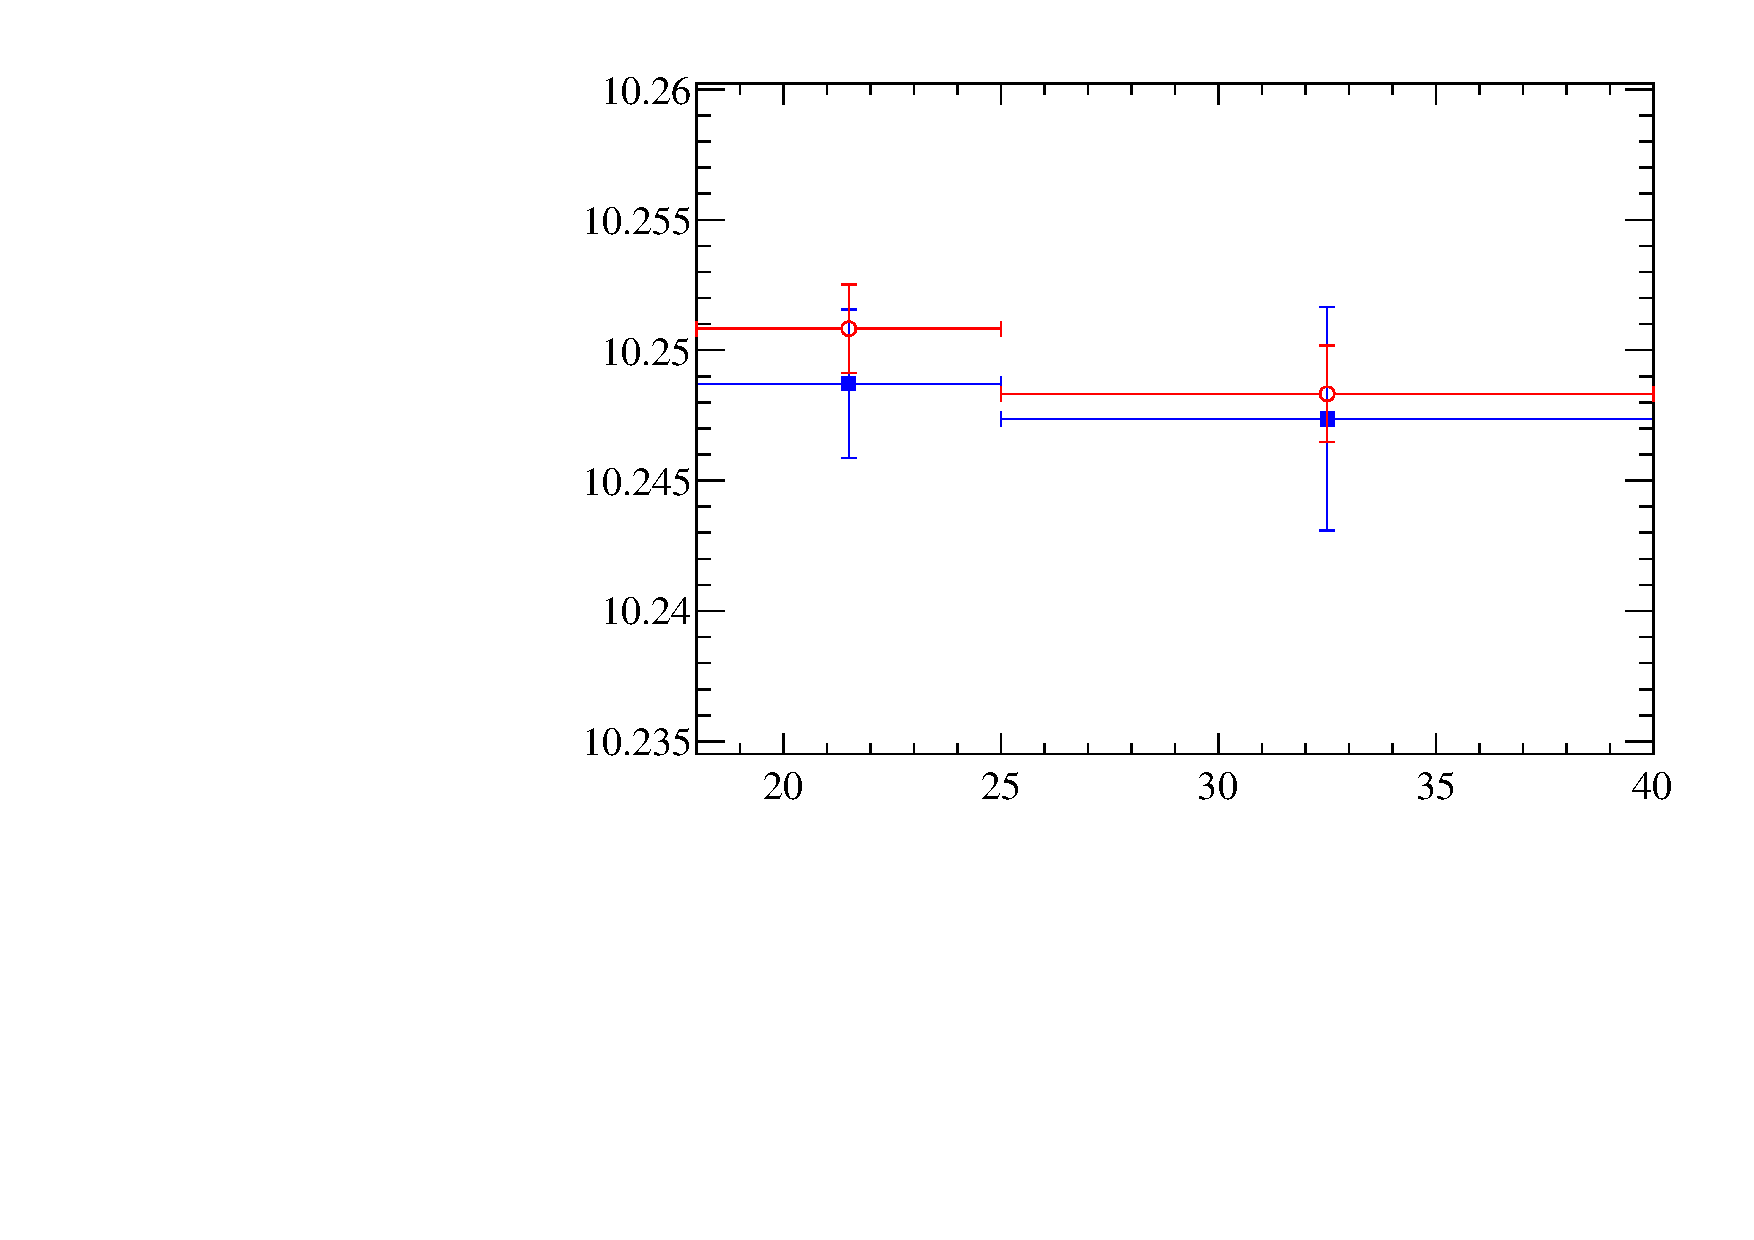
\includegraphics[width=70mm, height=50mm]{chib2s-m/m2p_2s}
}

\put(27, 40){\textcolor{blue}{\sqs=7\tev}, \textcolor{red}{\sqs=8\tev}}
\put(0,12){\begin{sideways}\chiboneTwoP mass \gevcc\end{sideways}}
\put(20,1){$p_T(\Upsilon) \left[\gevc\right]$}

%\put(0,12){\begin{sideways}Candidates\end{sideways}}
%\put(17,0){$p_T(\Upsilon) \left[\gevc\right]$}
%\put(35,30){\ThreeS}

%    \put(12,0){\tiny $m(\mumu) \left[\gevcc\right]$}
     
%\graphpaper[5](0,0)(50, 40)        
\end{picture}


In this study the mass of \chiboneTwoP was fixed to \textcolor{blue}{10249} \mevcc.

\end{center}
\end{frame}


\begin{frame}{$\chi_b$ yields in $\chi_b \to \TwoS$ decays}
  \setlength{\unitlength}{1mm}
  \centering
  \scalebox{0.7}{
  \begin{picture}(150,60)
    \put(0,0){
      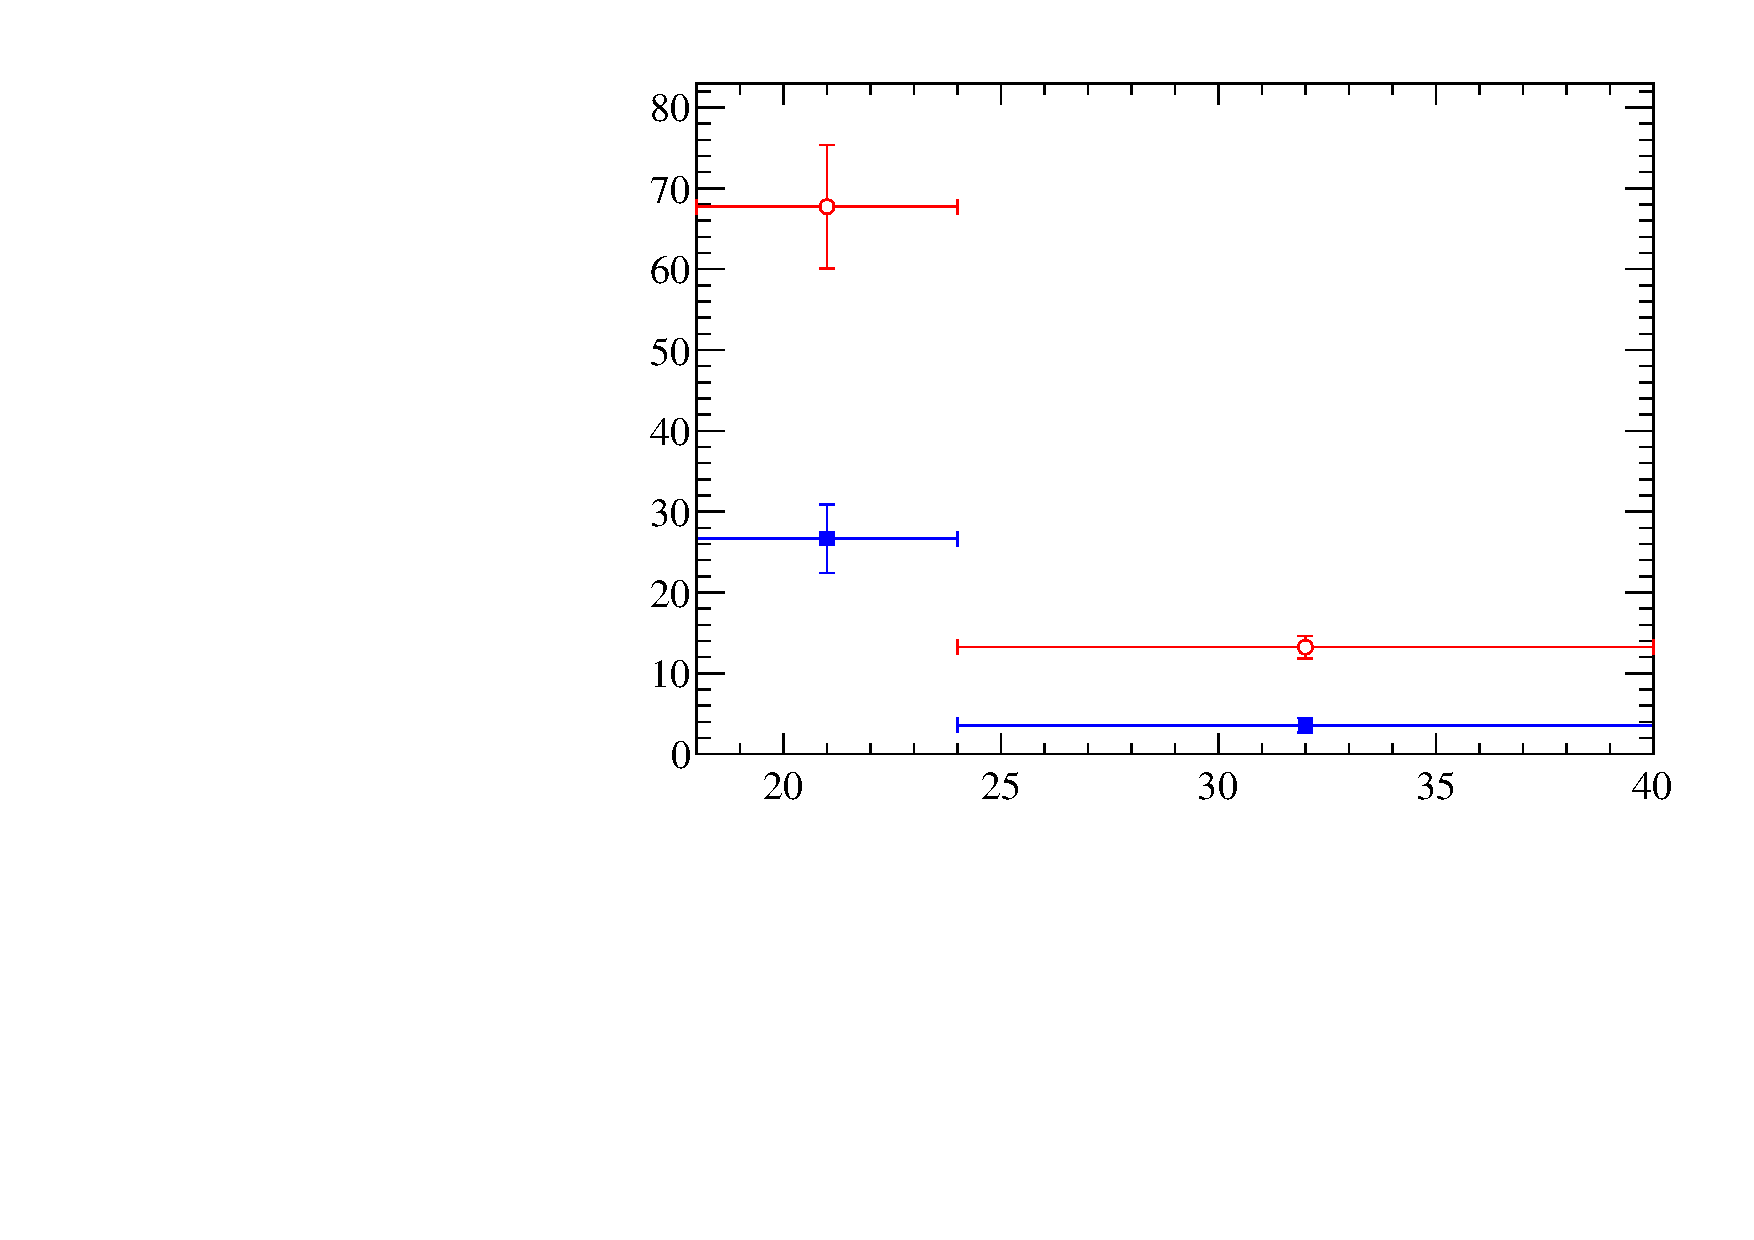
\includegraphics[width=75mm, height=60mm]{chib2s-yields/yields_2p}
    }
    \put(75,0){
      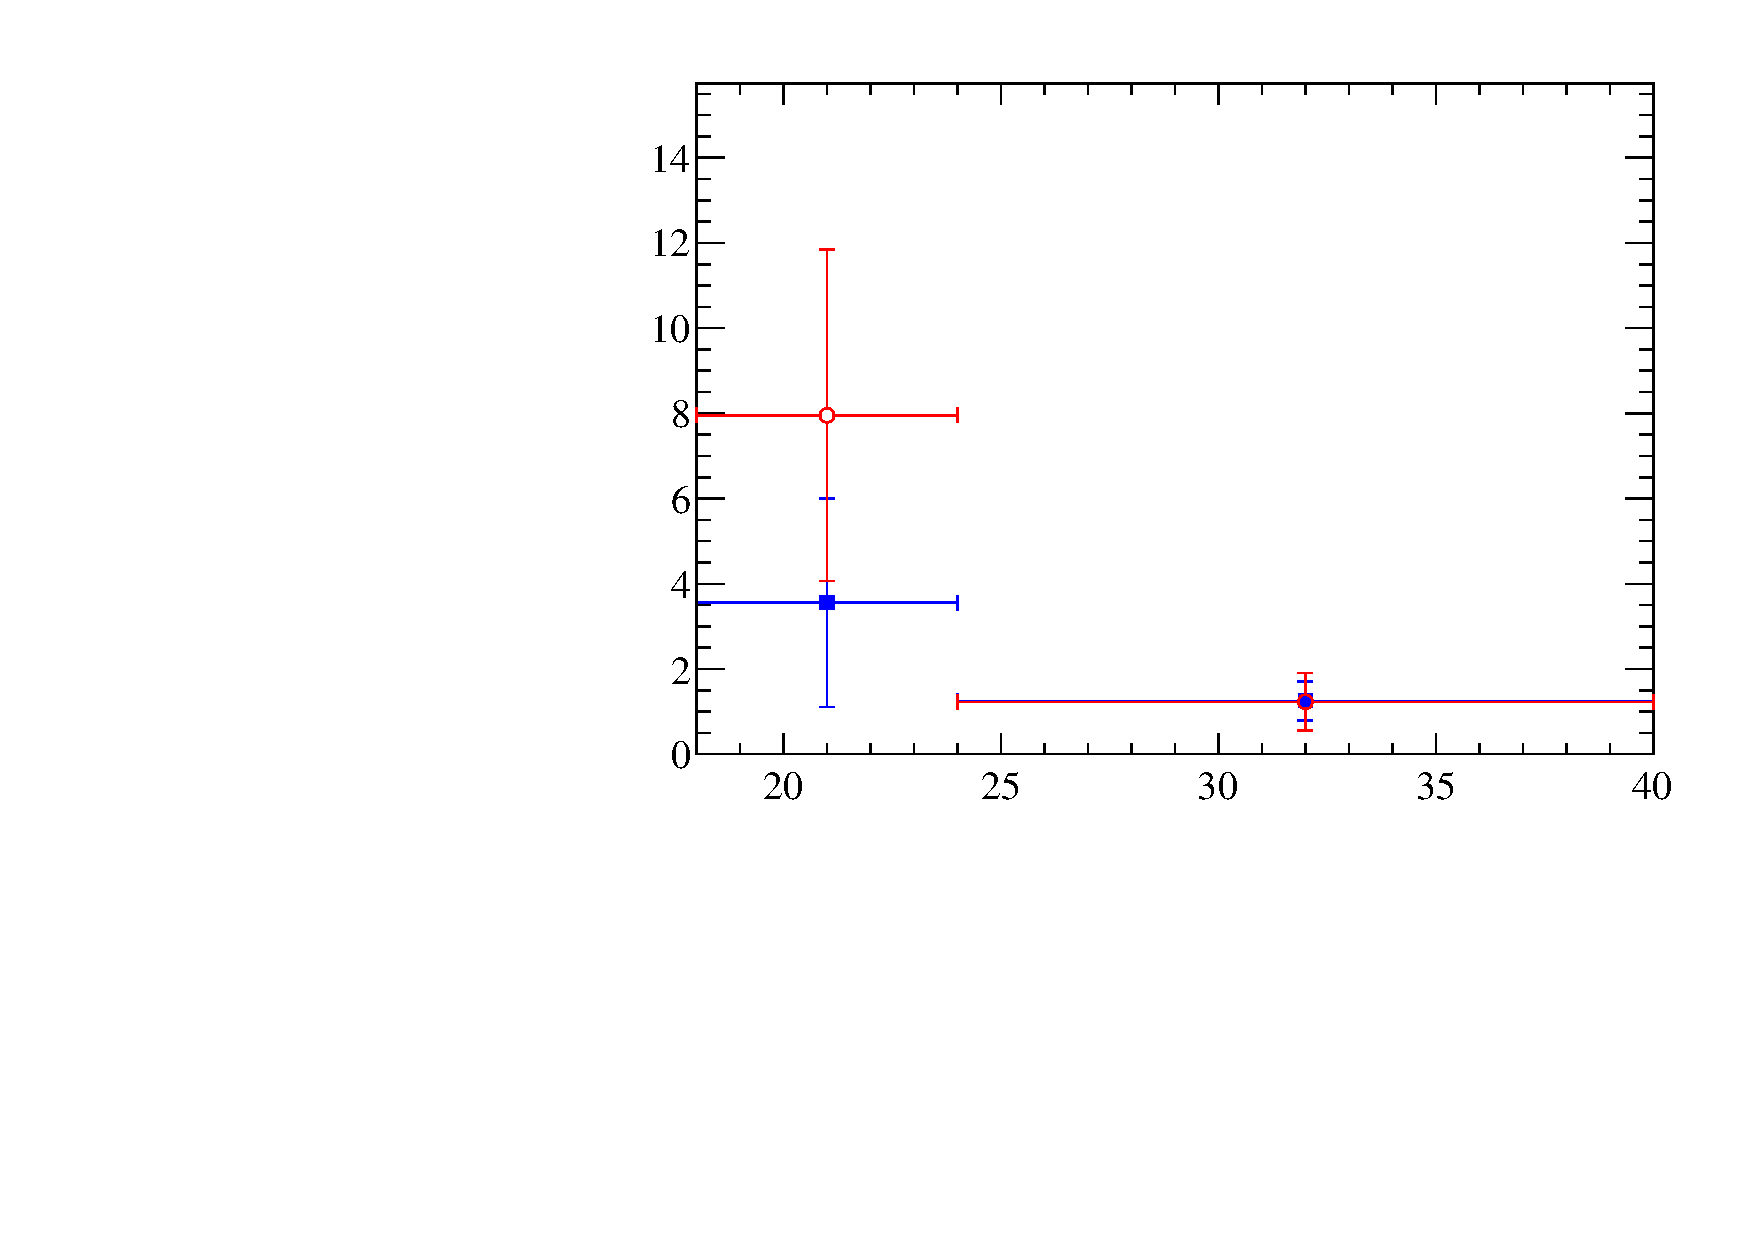
\includegraphics[width=75mm, height=60mm]{chib2s-yields/yields_3p}
    }


    \put(2,25){\begin{sideways}Events\end{sideways}}
    \put(35,2){$p_T^{\Y2S} \left[\gevc\right]$}
    \put(55,50){$\chibTwoP$}

    \put(77,25){\begin{sideways}Events\end{sideways}}
    \put(110,2){$p_T^{\Y2S} \left[\gevc\right]$}
    \put(130,50){$\chibThreeP$}


    \put(50,45){\textcolor{blue}{\sqs=7\tev}}
    \put(50,40){\textcolor{red}{\sqs=8\tev}}
    \put(45,45){
      
\includegraphics[width=3mm, height=2mm]{bsf}
    }
    \put(45,40){
      
\includegraphics[width=3mm, height=2mm]{rco}
    }

    \put(125,45){\textcolor{blue}{\sqs=7\tev}}
    \put(125,40){\textcolor{red}{\sqs=8\tev}}
    \put(120,45){
      
\includegraphics[width=3mm, height=2mm]{bsf}
    }
    \put(120,40){
      
\includegraphics[width=3mm, height=2mm]{rco}
    }

  % \graphpaper[5](0,0)(75, 60)
  \end{picture}
}
\begin{center}
Yields normilized by bin width.
\end{center}
\end{frame}


\begin{frame}{$\chi_{b1,2}(3P) \to \ThreeS$ fit model}
\begin{columns}[T]
\column{.5\textwidth}
  \centering
  \setlength{\unitlength}{1mm}
  \begin{picture}(50,80)
      %
    \put(0,0){
      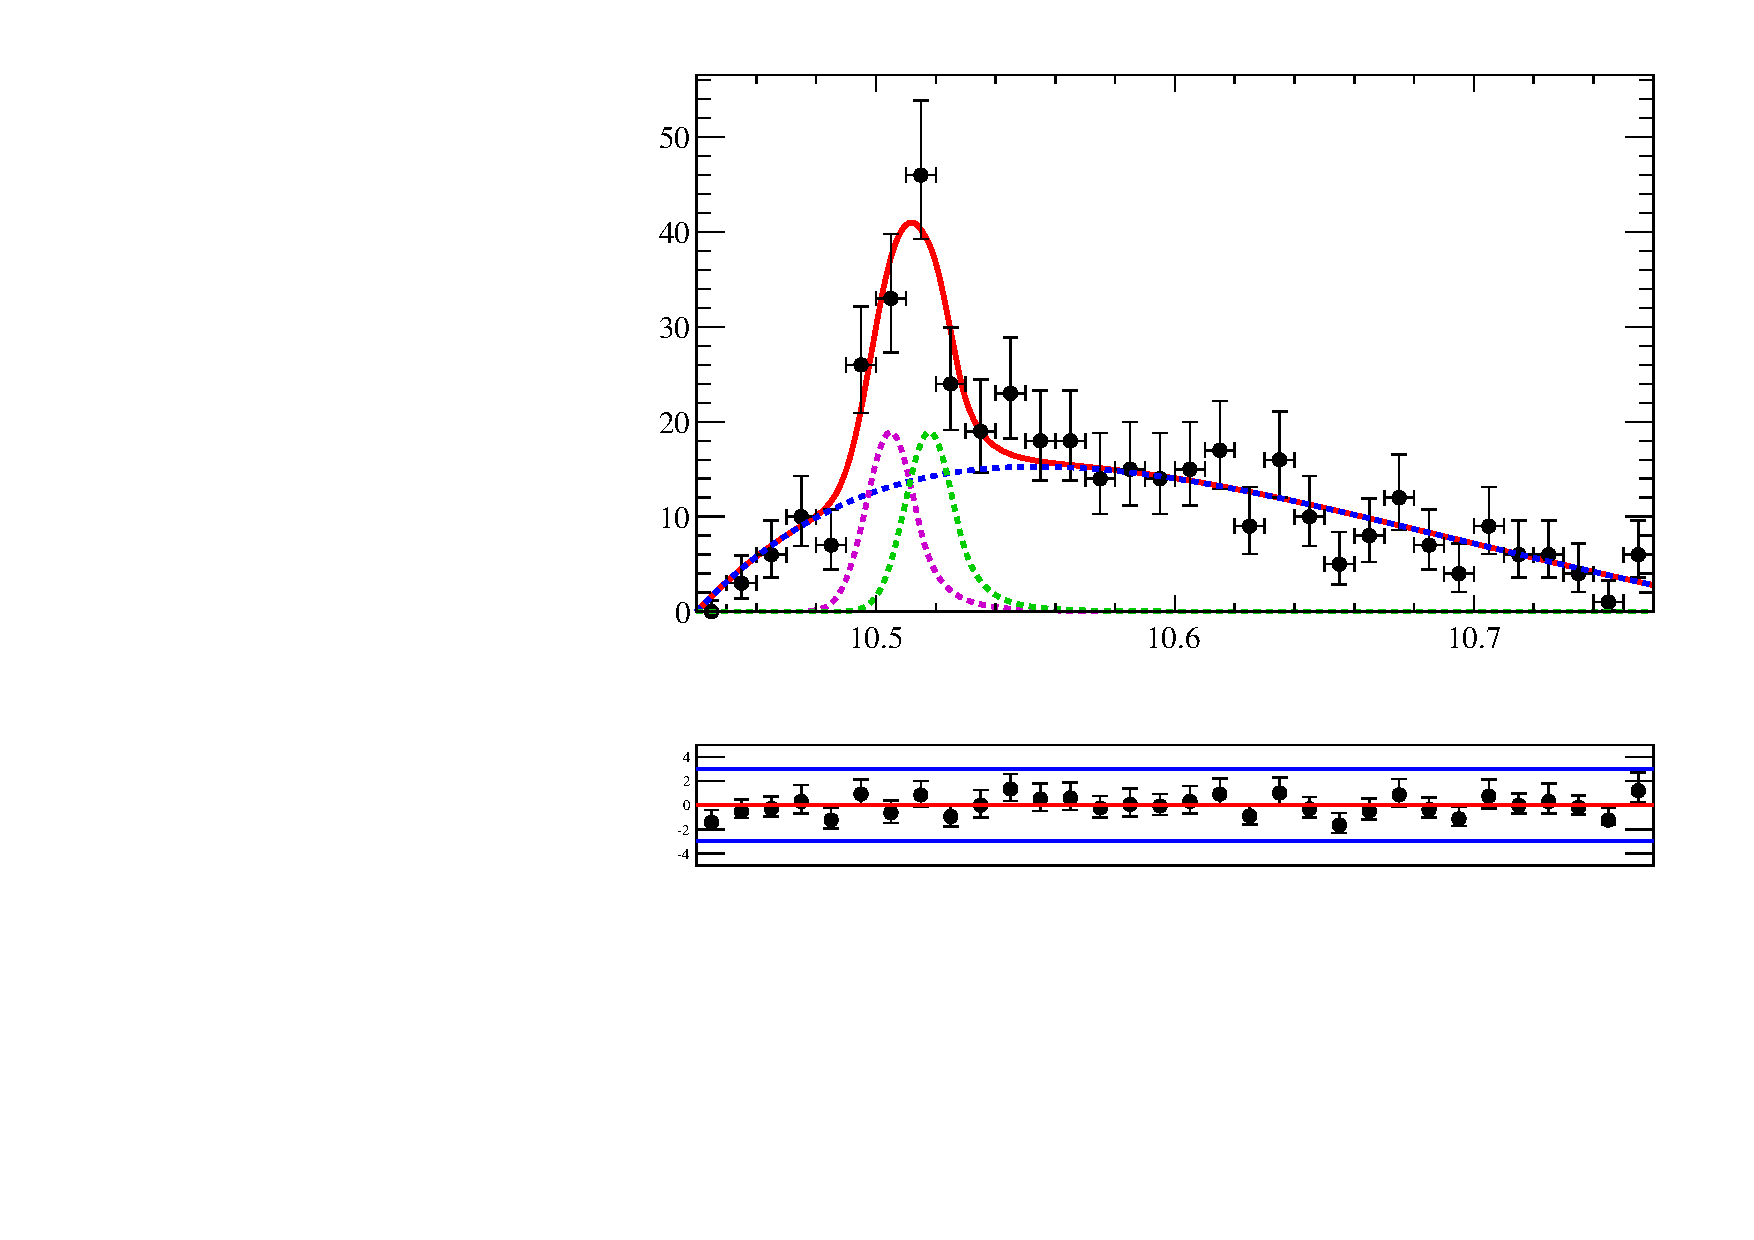
\includegraphics[width=50mm, height=40mm]{chib3s-fit/f2012_fix_27_None}
    }
    
    \put(0,40){
      \includegraphics[width=50mm, height=40mm]{chib3s-fit/f2011_fix_27_None}
    }

    \put(0,15){\tiny \begin{sideways}Candidates/(20\mevcc)\end{sideways}}
    \put(2,9.5){\tiny $m_{\mumu \gamma} - m_{\mumu} + 10.3552 \left[\gevcc\right]$}
    \put(25,30){$\sqrt{s} = 8 \gev$}
    \put(20,25){\tiny $p_T(\Y3S) > 27 \gevc$}    
    
    \put(0,55){\tiny \begin{sideways}Candidates/(20\mevcc)\end{sideways}}
    \put(2, 49.5){\tiny $m_{\mumu \gamma} - m_{\mumu} + 10.3552 \left[\gevcc\right]$}
    \put(25,70){$\sqrt{s} = 7 \gev$}     
    \put(20,65){\tiny $p_T(\Y3S) > 27 \gevc$}        
    %\graphpaper[2](0,0)(50, 40)        
  \end{picture}
\column{.5\textwidth}
\begin{itemize}
\item 2 Crystal Ball for each of $\chi_{b1,2}(3P)$ signal.
\item Product of exponential and linear compination of basic Bernstein polinomials  for combinatorial background.
\end{itemize}
\end{columns}
\end{frame}

\begin{frame}{$\chi_{b1,2}(3P) \to \ThreeS$ fit model (2)}
\begin{columns}[T]
\column{.5\textwidth}
\begin{itemize}
\item Free parameters: $\mu_{\chi_{b1}(3P)}$, yields and background parameters.
\item Linked parameters for \chibone and \chibtwo signals:
    \begin{itemize}
    \item $\mu_{\chi_{b2}(3P)} = \mu_{\chi_{b1}(3P)} + \Delta m_{\chi_{b2}(3P)}^{theory}$
    \item $N_{\chi_{b}} = \lambda N_{\chi_{b1}} + (1-\lambda) N_{\chi_{b2}}$
    \item $\sigma_{\chi_{b2}} = \sigma_{\chi_{b1}}$
    \end{itemize}

\item Fixed parameters from MC study:
    \begin{itemize}
    \item $\sigma_{\chiboneThreeP}$
    \item $\alpha$ and $n$ parameters of CB.
    \end{itemize}
\end{itemize}
\column{.5\textwidth}
\scalebox{0.42}{
    \begin{tabular}{lrrr}\toprule
    & \multicolumn{ 3 }{c}{\ThreeS transverse momentum intervals} \\
     & & \multicolumn{2}{c}{$p_T(\Y3S)> 27 \gevc$} \\
    \cmidrule{3-4}
     && \sqs = 7 \tev & \sqs = 8\tev \\
    \midrule
    $N_{\chi_{b}(3P)}$  && 34 $\pm$ 8 & 82 $\pm$ 14 \\
    $B$  && 114 $\pm$ 12 & 329 $\pm$ 21 \\

    \rule{0pt}{4ex}$\mu_{\chi_{b1}(3P)}, \mevcc$  && \textcolor{blue}{10,514.5 $\pm$ 3.0} & \textcolor{blue}{10,504.9 $\pm$ 2.2} \\

    \rule{0pt}{4ex}$\Delta m_{\chi_{b2,1}(3P)}, \mevcc$  && \multicolumn{2}{c}{13.00} \\

    $\sigma_{\chi_{b1}(3P)}, \mevcc$  && \multicolumn{2}{c}{8.03} \\

    \rule{0pt}{4ex}$\lambda_{\chibThreeP}$  && \multicolumn{2}{c}{0.5} \\

    \rule{0pt}{4ex}$\alpha_{\chi_{b}(3P)}$  && \multicolumn{2}{c}{-1.25} \\
    $n_{\chi_{b}(3P)}$  && \multicolumn{2}{c}{5.0} \\

    \rule{0pt}{4ex}$\tau$  && -8 $\pm$ 7 & -4.8 $\pm$ 1.4 \\
    $c_0$  && 0.62 $\pm$ 0.09 & 0.62 $\pm$ 0.08 \\
    $c_1$  && 0.1 $\pm$ 0.6 & -0.33 $\pm$ 0.12 \\

    \rule{0pt}{4ex}$\chi^2 / n.d.f$  && 0.6 & 0.8 \\
    \bottomrule
\end{tabular}
}
%
\bigskip

In this study the mass of $\chi_{b1}(3P)$ was fixed to the value obtained from
the fit performed on both datasets =  \textcolor{blue}{10507$\pm$2}~\mevcc
\end{columns}


\end{frame}

\begin{frame}{$m_{\chi_{b1}(3P)}$ in study with  converted photons}
\begin{center}
The measured $m_{\chiboneThreeP}$ (10,507$\pm$2\mevcc) is consistent with the mass measured in another study with converted photons (10,509$\pm$3.0\mevcc).
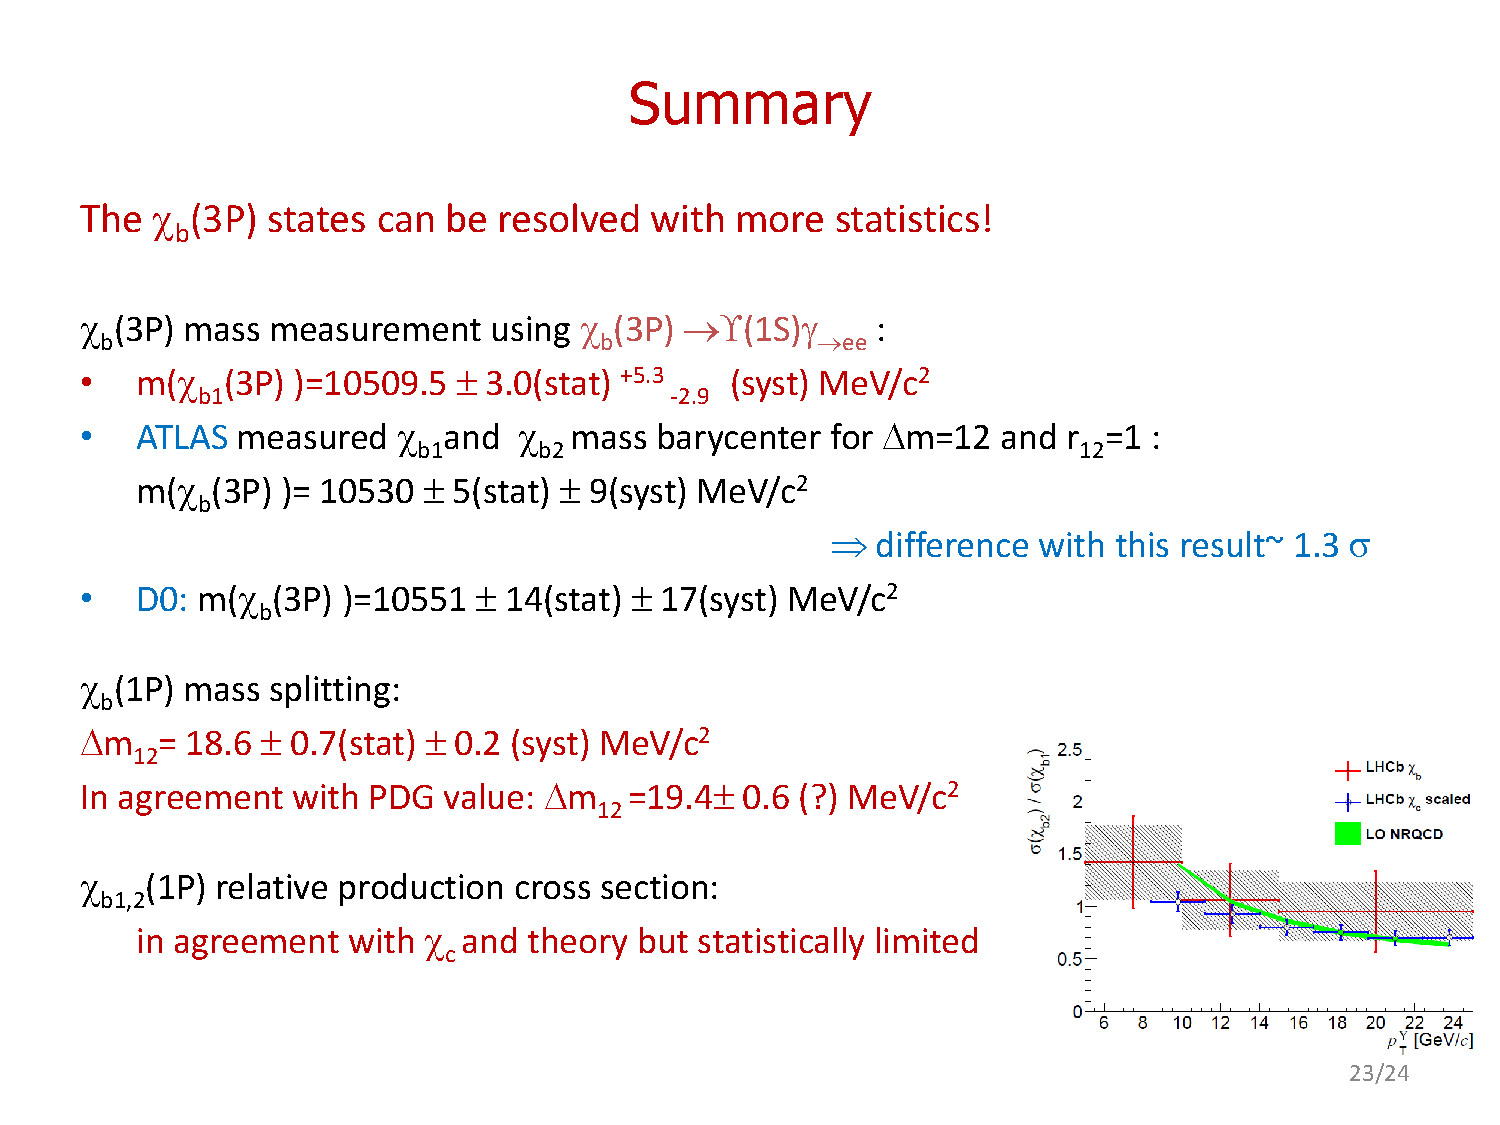
\includegraphics[width=85mm]{m3p-converted/converted}
\end{center}
\end{frame}

\begin{frame}{MC efficiency (1)}
\setlength{\unitlength}{1mm}
\begin{center}
MC true events $\chi_b(3P) \to \Y1S \gamma$ (other decays have the same shape)
\begin{picture}(70,50)
      %
    \put(0,0){
      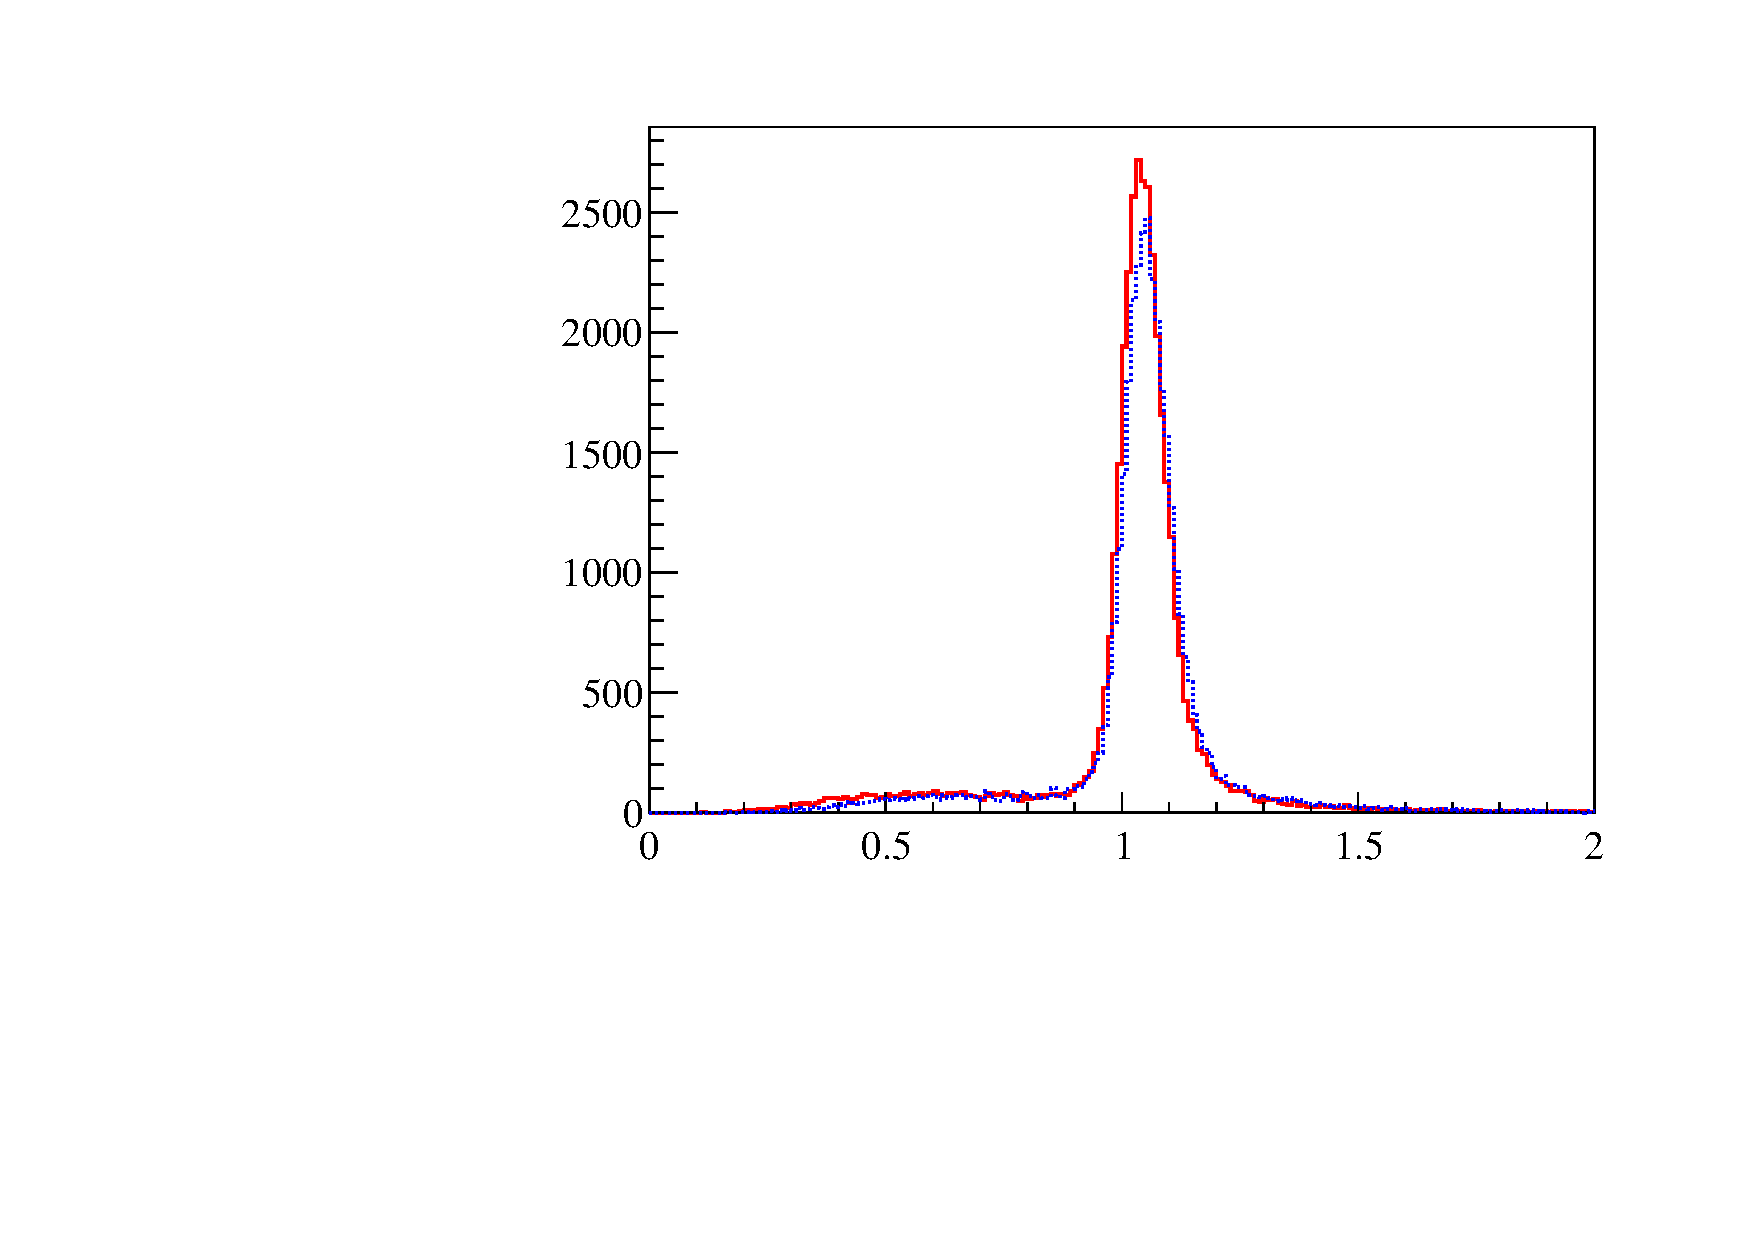
\includegraphics[width=70mm, height=50mm]{mc-fits/cb3_h}
    }
    
%    \put(0,40){
%      \includegraphics[width=50mm, height=40mm]{7.1-chib3s-fit/f2011_fix_27_None}
%    }

    \put(0,12){\begin{sideways}Candidates\end{sideways}}
    \put(20,0){$m_{\mumu \gamma} - m_{\mumu} \left[\gevcc\right]$}

%    
%    \put(0,55){\tiny \begin{sideways}Candidates/(20\mevcc)\end{sideways}}
%    \put(2, 49.5){\tiny $m_{\mumu \gamma} - m_{\mumu} + 10.3552 \left[\gevcc\right]$}
%    \put(25,70){$\sqrt{s} = 7 \gev$}     
%    \graphpaper[2](0,0)(70, 50)        
  \end{picture}
 \end{center}
 
\begin{alertblock}{}
Monte-Carlo events in the flat left band are fitted as
background in the model for real data. So efficiency needs to be calculated with \chib mc-true events fitted by Crystal Ball function and some background which fits this band. 
$\Upsilon$ events are measured by counting mc-true events.

\end{alertblock}

\end{frame}
\begin{frame}{Monte-Carlo photon reconstruction (2)}
Example of fits:
  \setlength{\unitlength}{1mm}
  \centering
  \scalebox{0.5}{
  \begin{picture}(225,120)
    \put(0,60){
      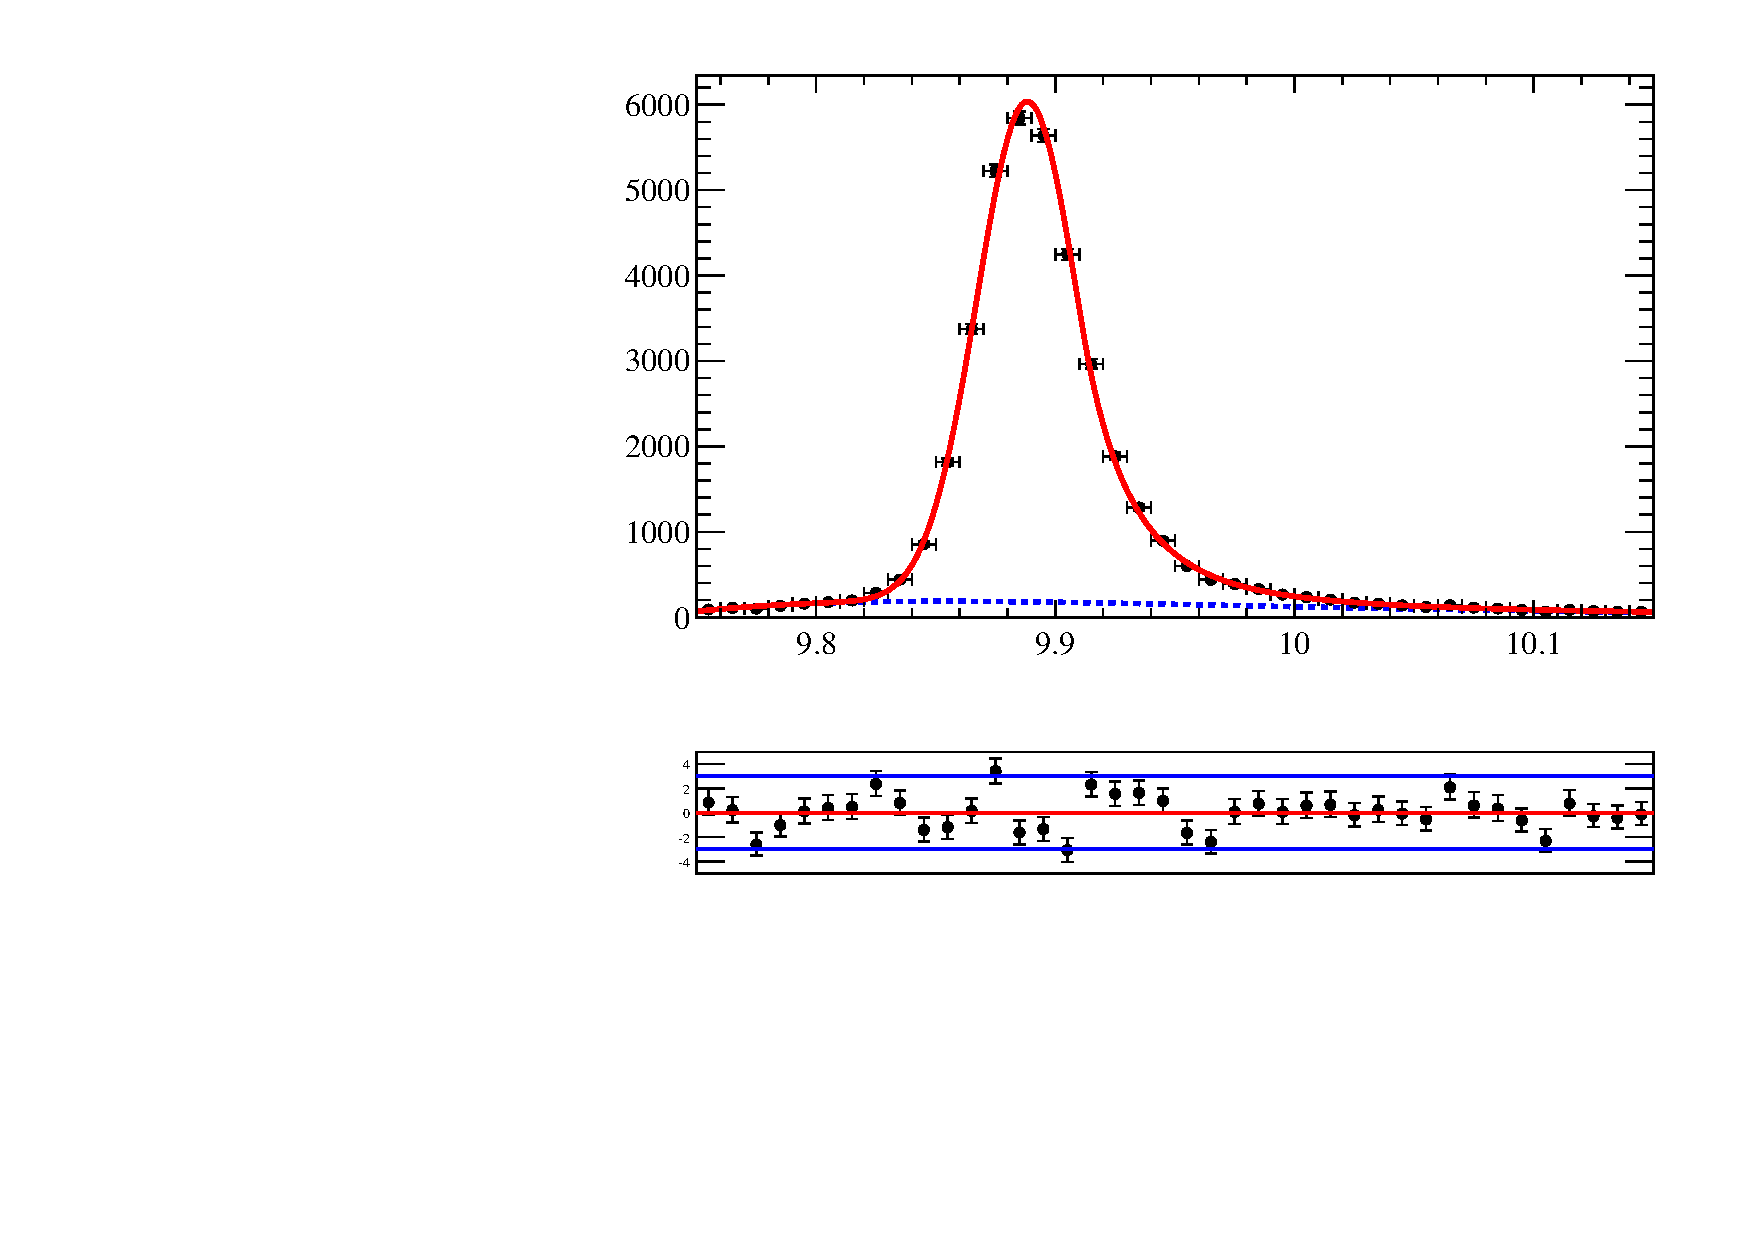
\includegraphics[width=75mm, height=60mm]{mc-fits-figs/cb11_6_40}
    }
    \put(42,114){\scriptsize $\chiboneOneP \to \Y1S \gamma$}
    \put(42,109){\scriptsize $6 < p_T^{\Y1S} < 40 \gevc$}
    \put(10,73){$m_{\mumu \gamma} - m_{\mumu} + 9.4603 \left[\gevcc\right]$}
    \put(3,85){\scriptsize \begin{sideways}Candidates/(10\mevcc)\end{sideways}}    
    \put(45,103){\scriptsize N = 34,330 $\pm$ 220}
    \put(45,100){\scriptsize B = 5240 $\pm$ 140 (13.3 $\pm$ 0.4\%)}
    

    \put(75,60){
      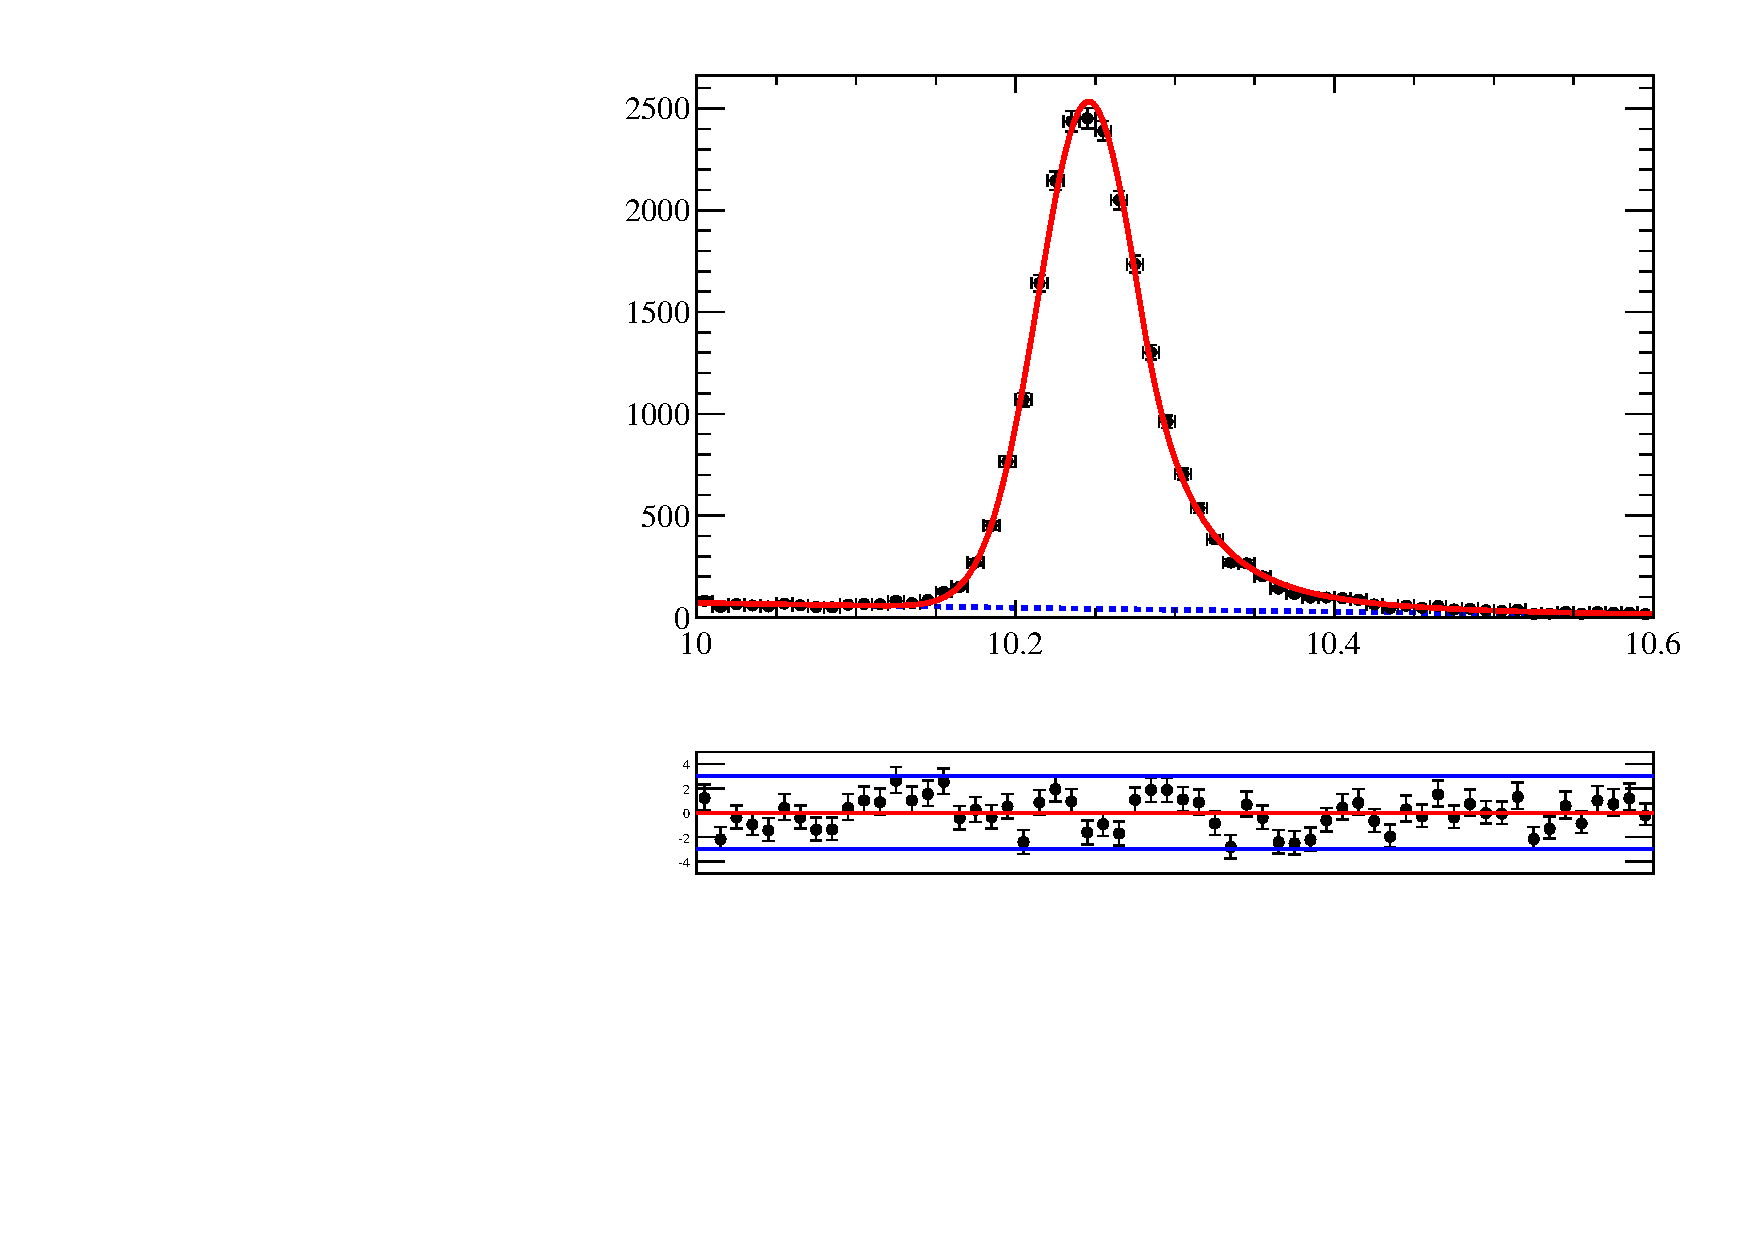
\includegraphics[width=75mm, height=60mm]{mc-fits-figs/cb12_6_40}
    }
    \put(117,114){\scriptsize $\chiboneTwoP \to \Y1S \gamma$}
    \put(117,109){\scriptsize $6 < p_T^{\Y1S} < 40 \gevc$}
    \put(85,73){$m_{\mumu \gamma} - m_{\mumu} + 9.4603 \left[\gevcc\right]$}
    \put(78,85){\scriptsize \begin{sideways}Candidates/(10\mevcc)\end{sideways}}    
    \put(120,103){\scriptsize N = 22,210 $\pm$ 170}
    \put(120,100){\scriptsize B = 2290 $\pm$ 90 (9.3 $\pm$ 0.4\%)}
    

    \put(150,60){
      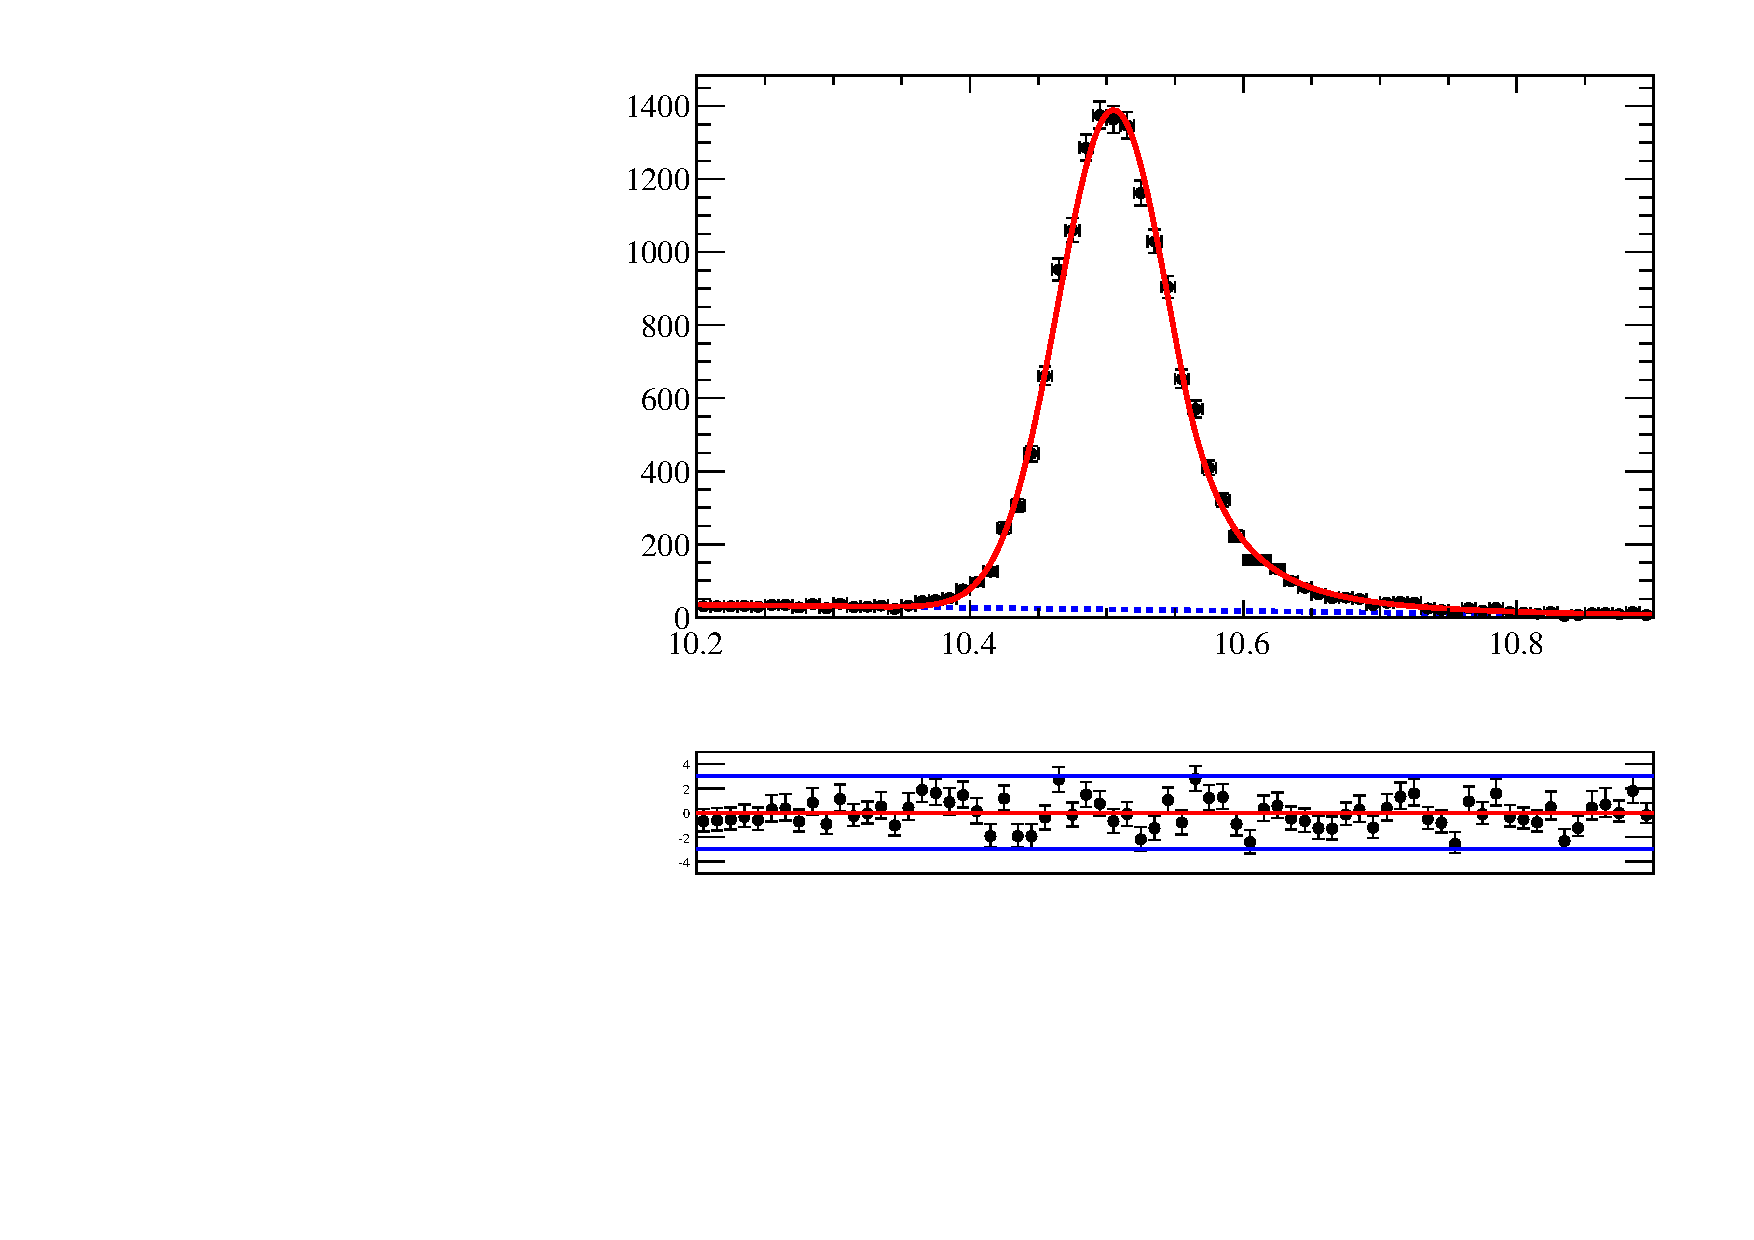
\includegraphics[width=75mm, height=60mm]{mc-fits-figs/cb13_6_40}
    }
    \put(192,114){\scriptsize $\chiboneThreeP \to \Y1S \gamma$}
    \put(192,109){\scriptsize $6 < p_T^{\Y1S} < 40 \gevc$}
    \put(160,73){$m_{\mumu \gamma} - m_{\mumu} + 9.4603 \left[\gevcc\right]$}
    \put(153,85){\scriptsize \begin{sideways}Candidates/(10\mevcc)\end{sideways}}    
    \put(195,103){\scriptsize N = 15,110 $\pm$ 130}
    \put(195,100){\scriptsize B = 1360 $\pm$ 60 (8.26 $\pm$ 0.35\%)}
    

    \put(0,0){
      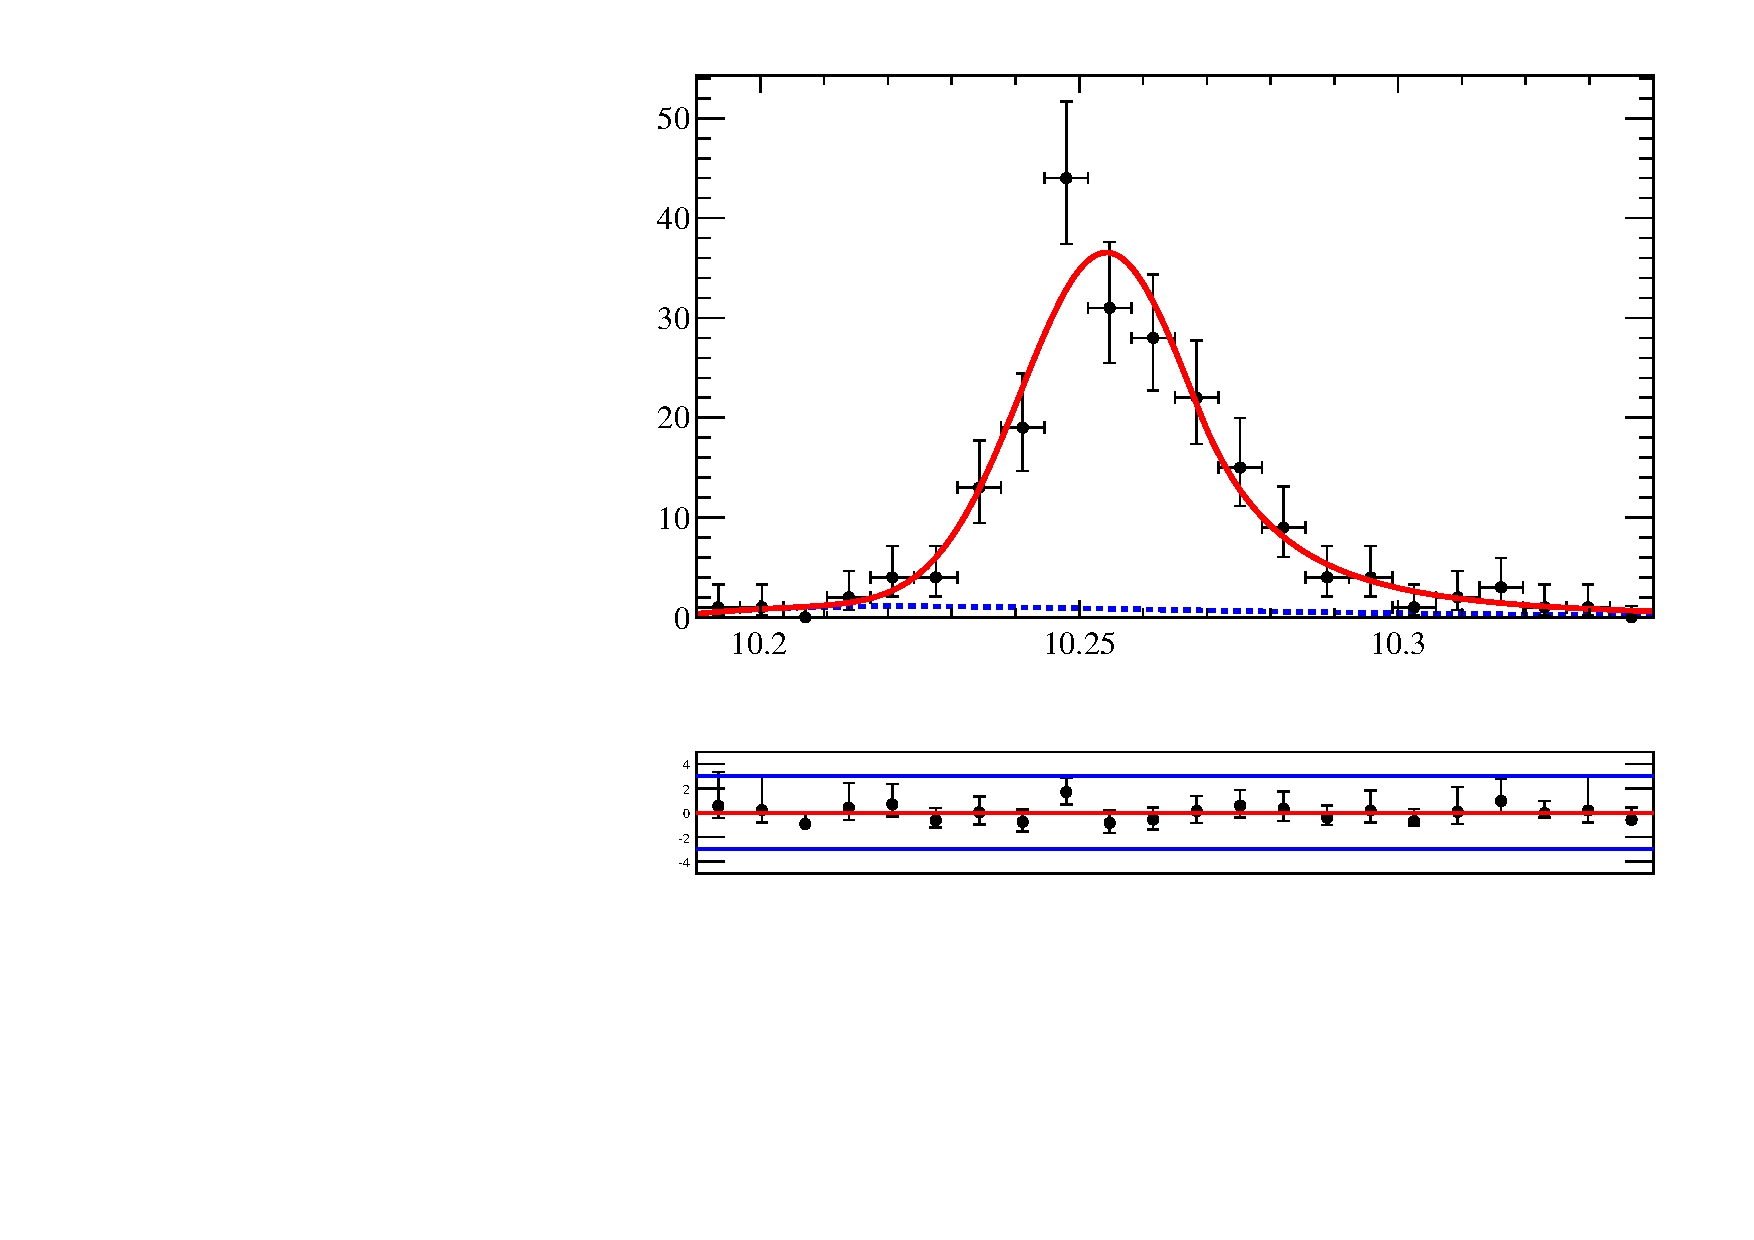
\includegraphics[width=75mm, height=60mm]{mc-fits-figs/cb12_18_40}
    }
    \put(42,54){\scriptsize $\chiboneTwoP \to \Y2S \gamma$}
    \put(42,49){\scriptsize $18 < p_T^{\Y1S} < 40 \gevc$}
    \put(10,13){$m_{\mumu \gamma} - m_{\mumu} + 10.02326 \left[\gevcc\right]$}
    \put(3,25){\scriptsize \begin{sideways}Candidates/(10\mevcc)\end{sideways}}    
    \put(45,43){\scriptsize N = 194 $\pm$ 21}
    \put(45,40){\scriptsize B = 15 $\pm$ 17 (7 $\pm$ 8\%)}
    

    \put(75,0){
      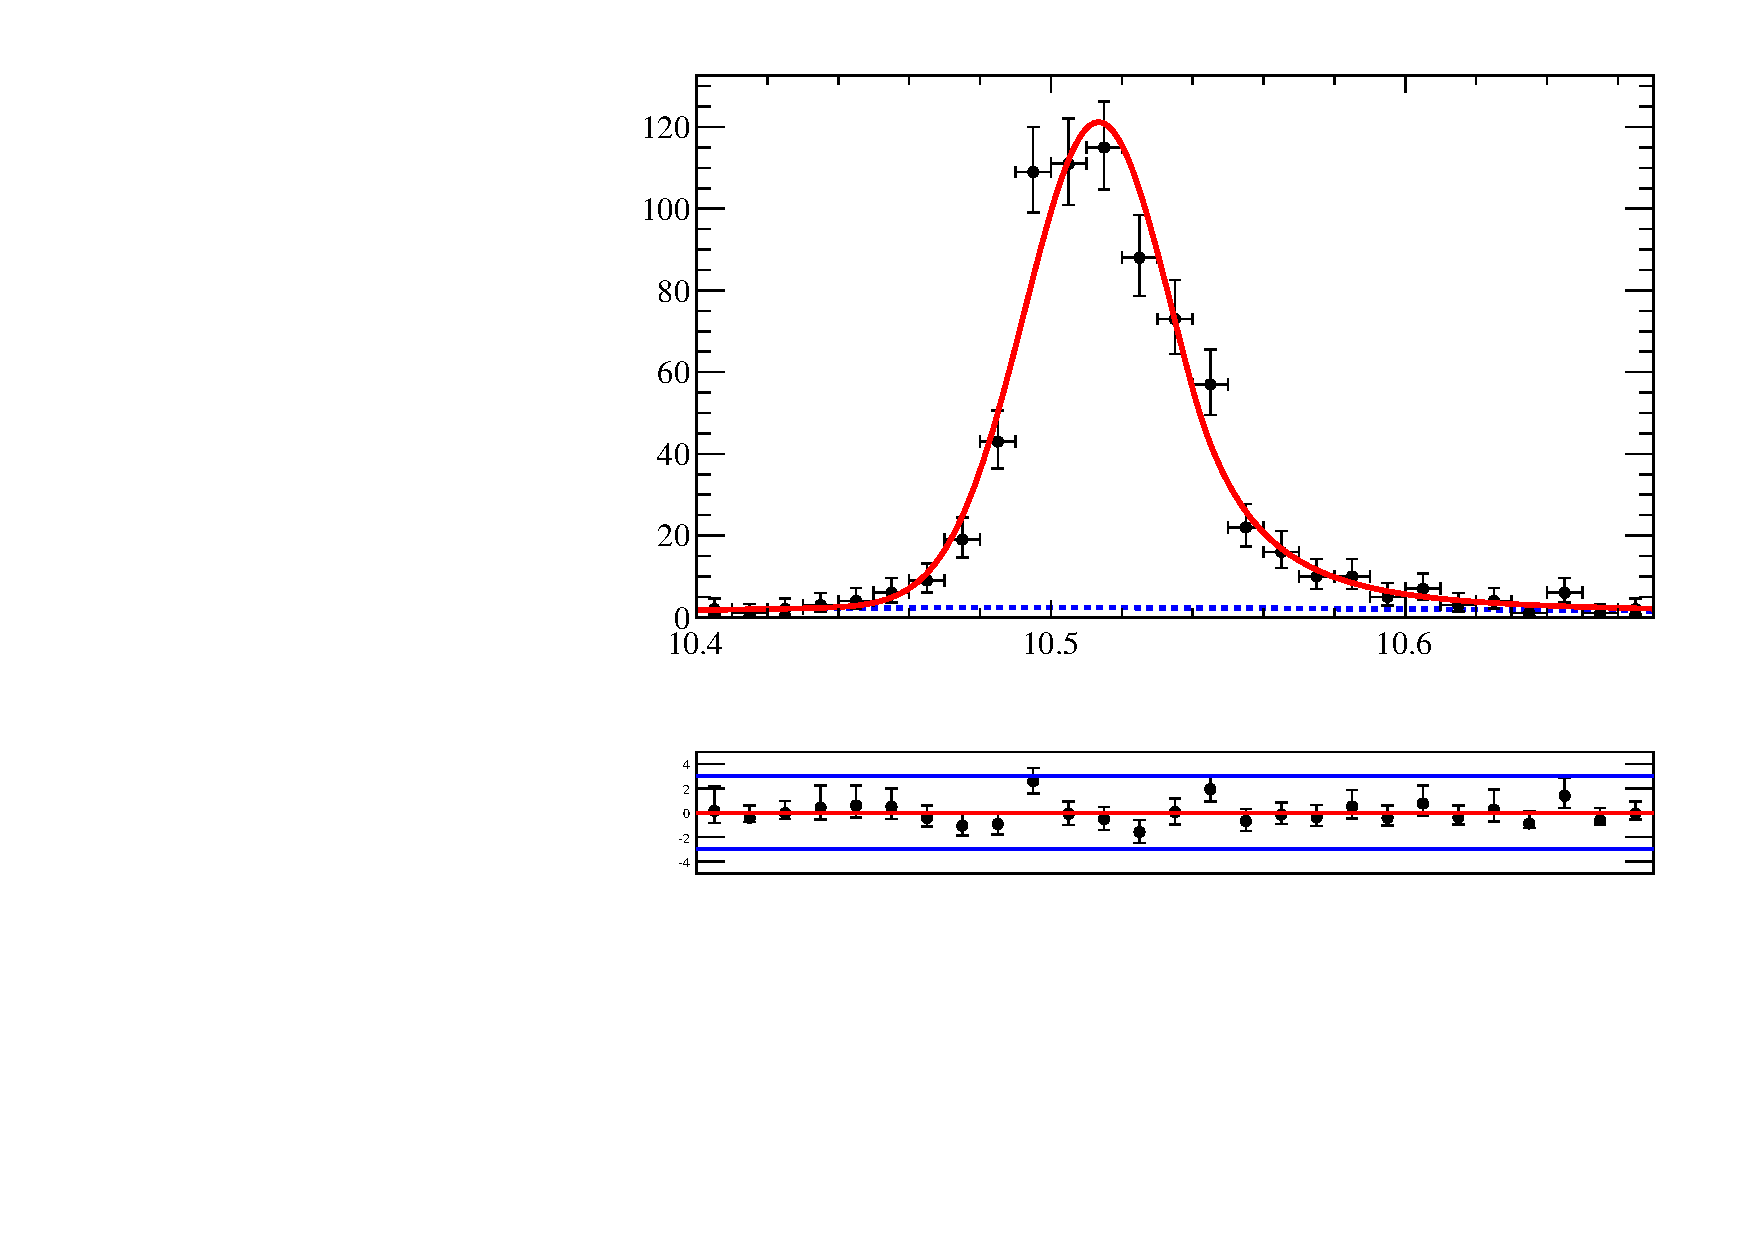
\includegraphics[width=75mm, height=60mm]{mc-fits-figs/cb13_18_40}
    }
    \put(117,54){\scriptsize $\chiboneThreeP \to \Y2S \gamma$}
    \put(117,49){\scriptsize $18 < p_T^{\Y1S} < 40 \gevc$}
    \put(85,13){$m_{\mumu \gamma} - m_{\mumu} + 10.02326 \left[\gevcc\right]$}
    \put(78,25){\scriptsize \begin{sideways}Candidates/(10\mevcc)\end{sideways}}    
    \put(120,43){\scriptsize N = 672 $\pm$ 32}
    \put(120,40){\scriptsize B = 57 $\pm$ 21 (7.8 $\pm$ 2.9\%)}
    

    \put(150,0){
      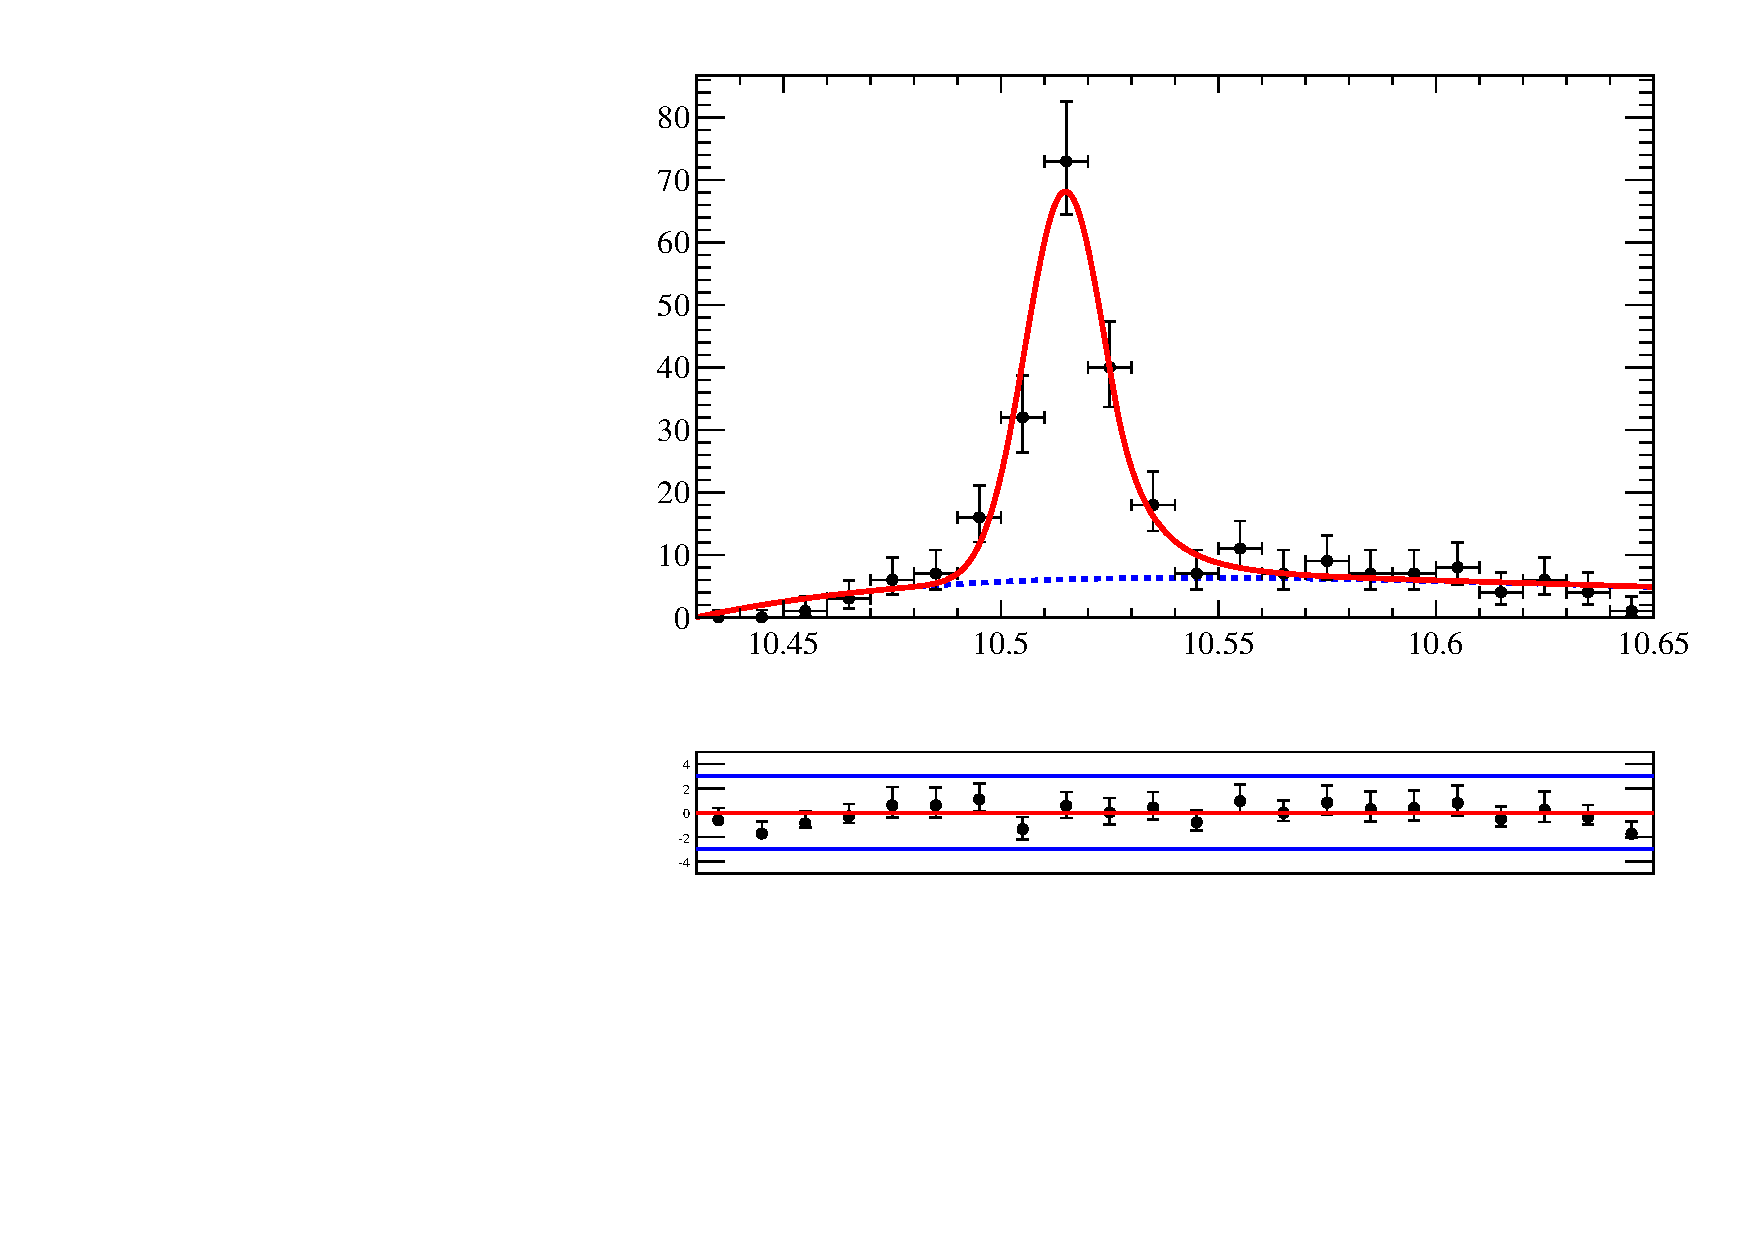
\includegraphics[width=75mm, height=60mm]{mc-fits-figs/cb13_27_40}
    }
    \put(192,54){\scriptsize $\chiboneThreeP \to \Y3S \gamma$}
    \put(192,49){\scriptsize $27 < p_T^{\Y1S} < 40 \gevc$}
    \put(160,13){$m_{\mumu \gamma} - m_{\mumu} + 10.355 \left[\gevcc\right]$}
    \put(153,25){\scriptsize \begin{sideways}Candidates/(10\mevcc)\end{sideways}}    
    \put(195,43){\scriptsize N = 154 $\pm$ 17}
    \put(195,40){\scriptsize B = 113 $\pm$ 16 (42 $\pm$ 7\%)}
    

     % \graphpaper[5](0,0)(225, 120)        
  \end{picture}
 }

\end{frame}
\begin{frame}{Data --- Monte Carlo comparison}
A comparison of the distribution of the relevant observables used in this
analysis was performed on real and simulated data, in order to assess the
reliability of Monte Carlo in computing efficiencies

\begin{center}
\scalebox{0.38}{
  \setlength{\unitlength}{1mm}
  \begin{picture}(150,140)
    %
    \put(0,0){
      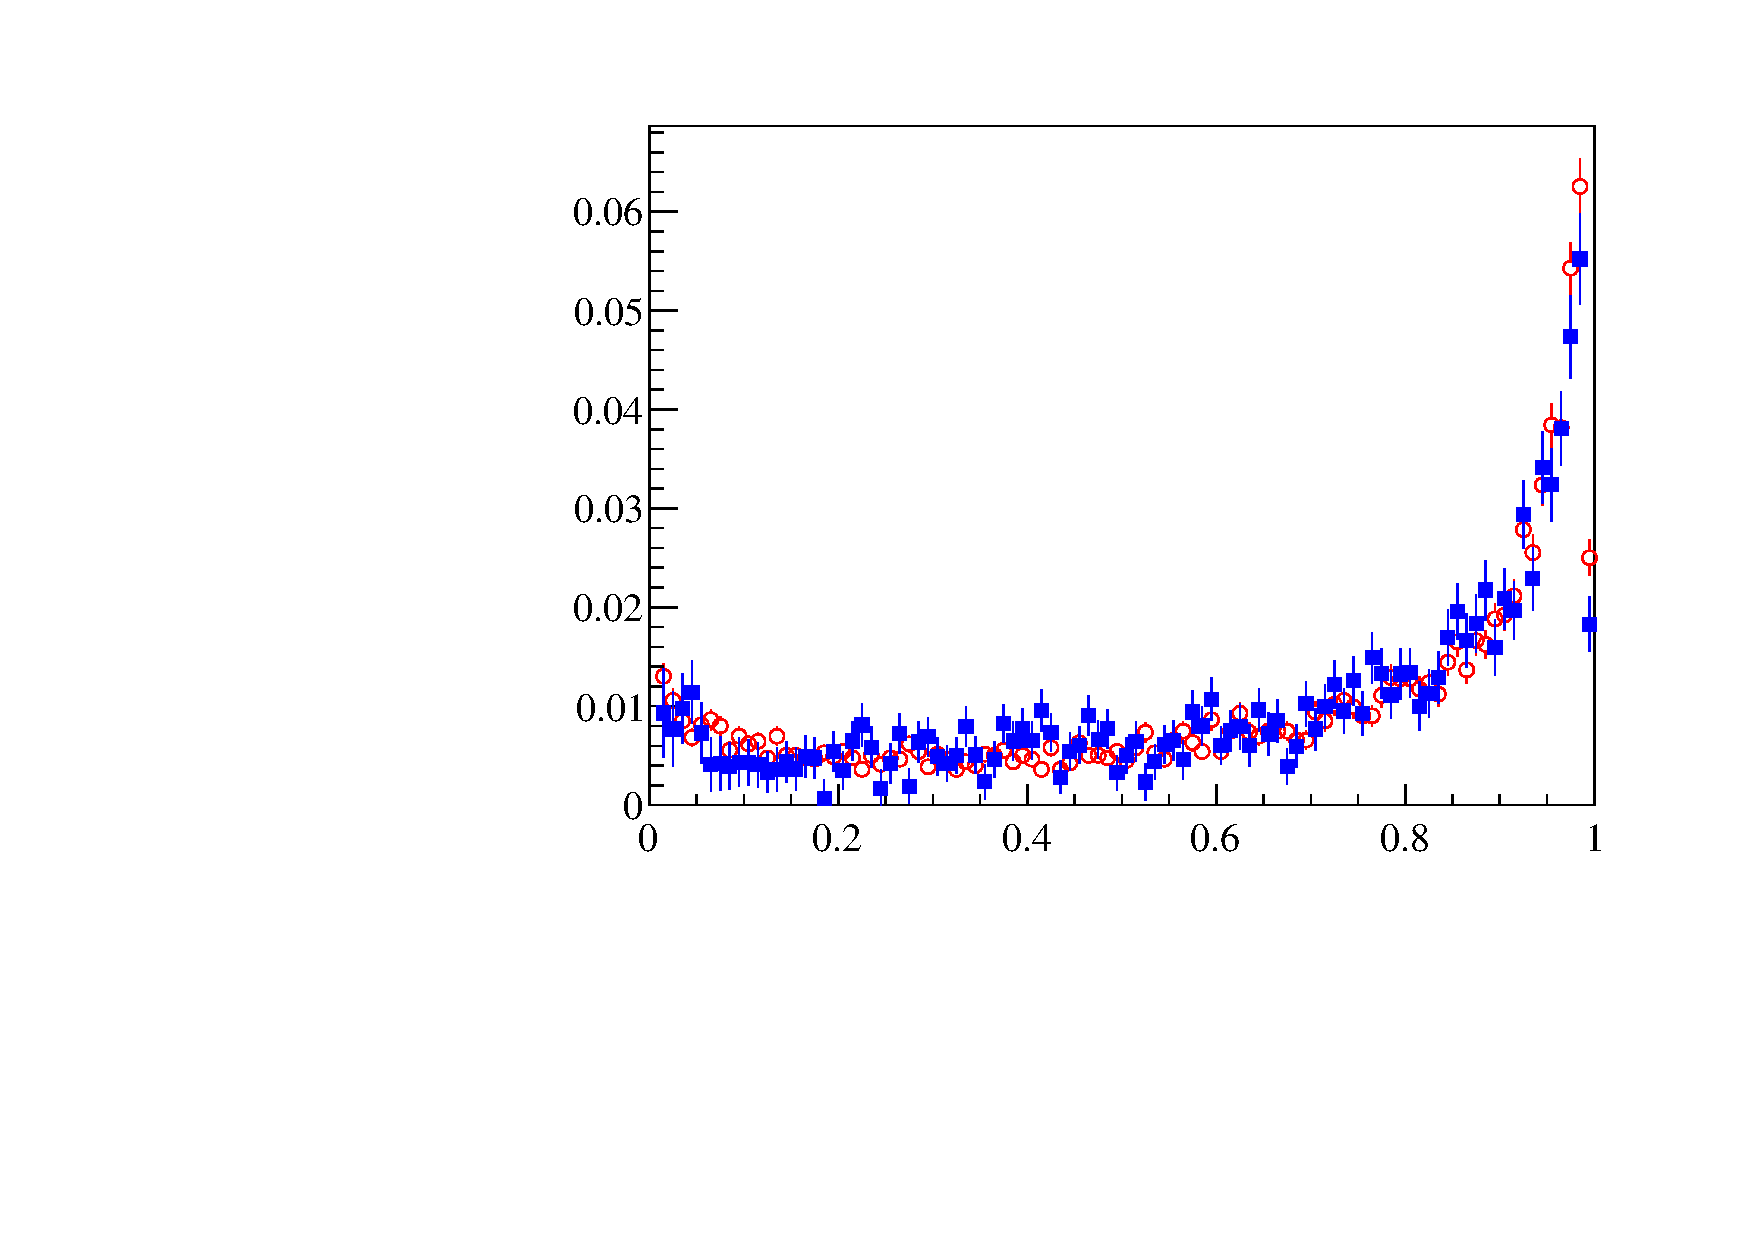
\includegraphics[width=50mm, height=35mm]{mc-data/cl_g_1p}
    }
    \put(50,0){
      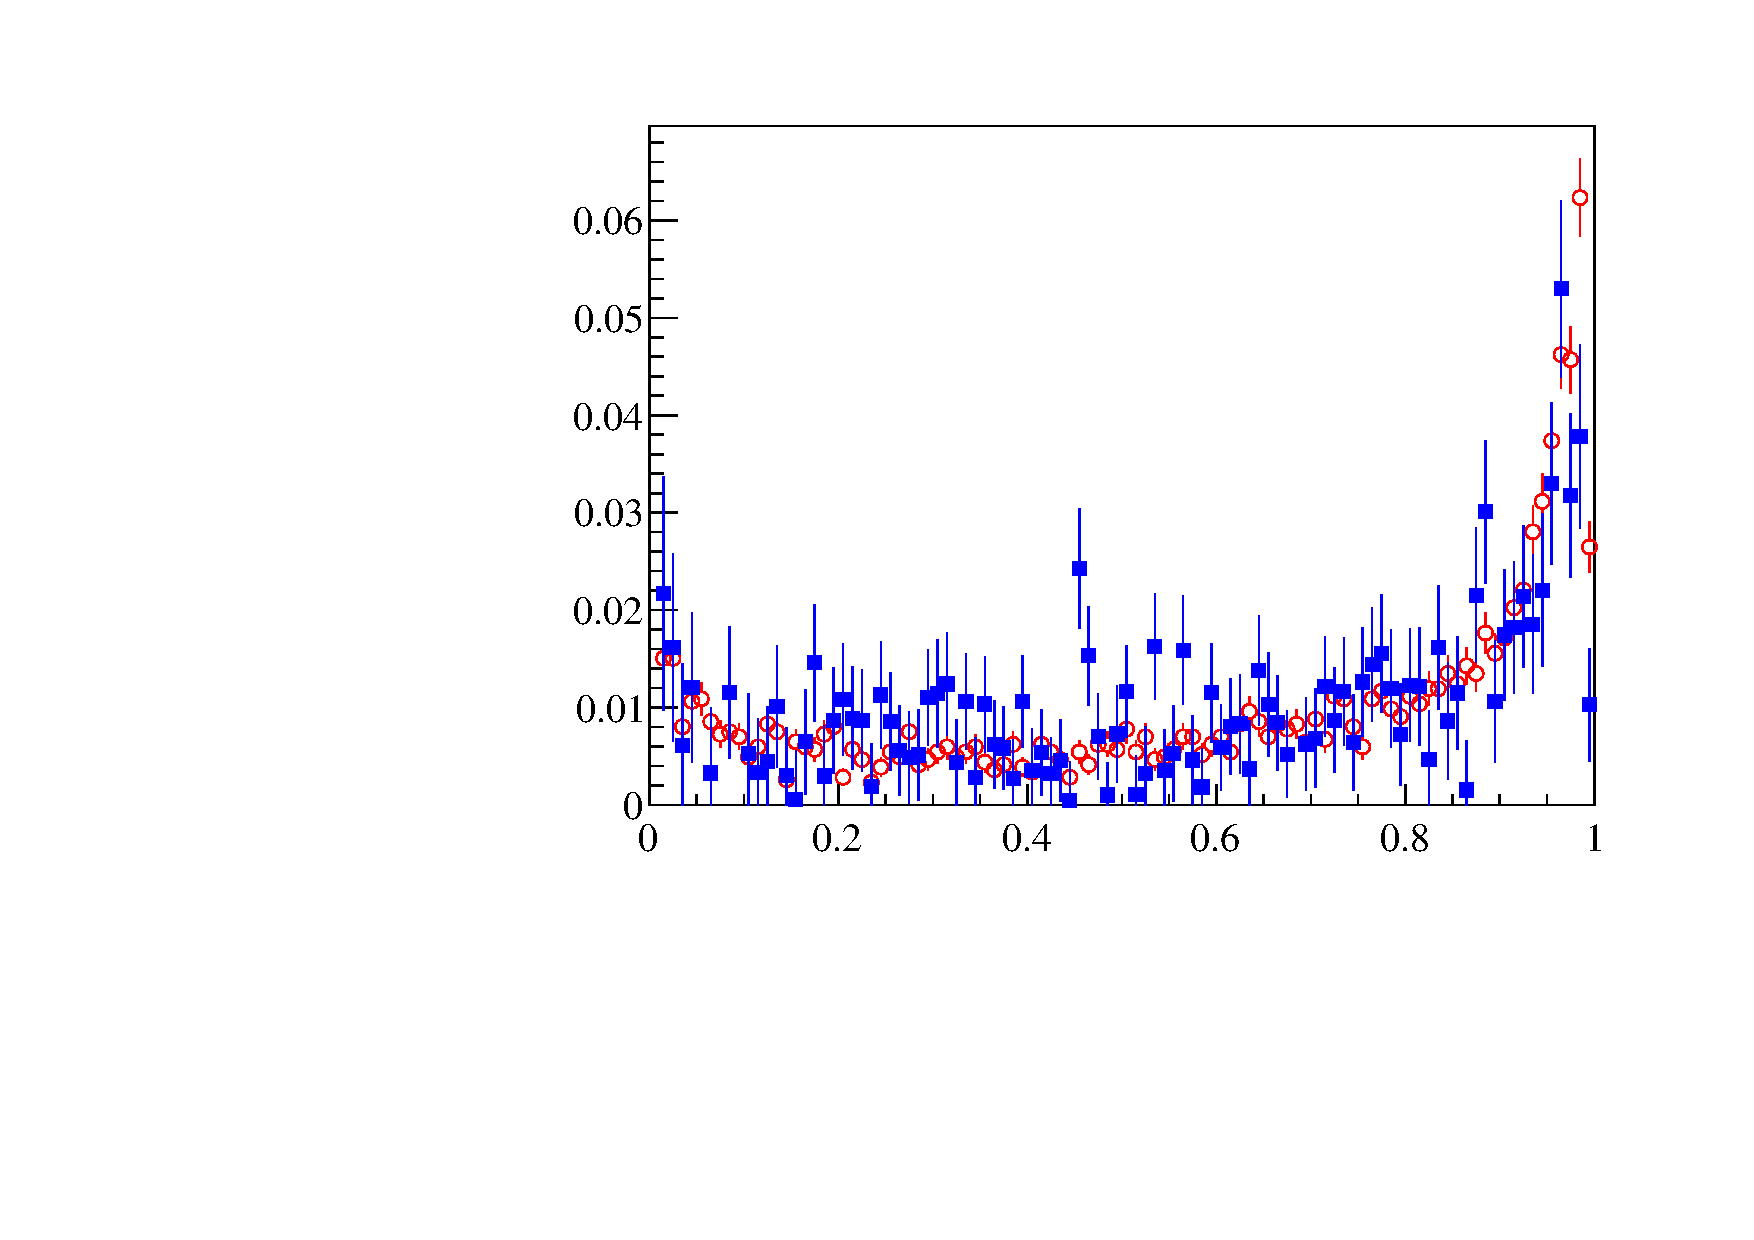
\includegraphics[width=50mm, height=35mm]{mc-data/cl_g_2p}
    }
    \put(100,0){
      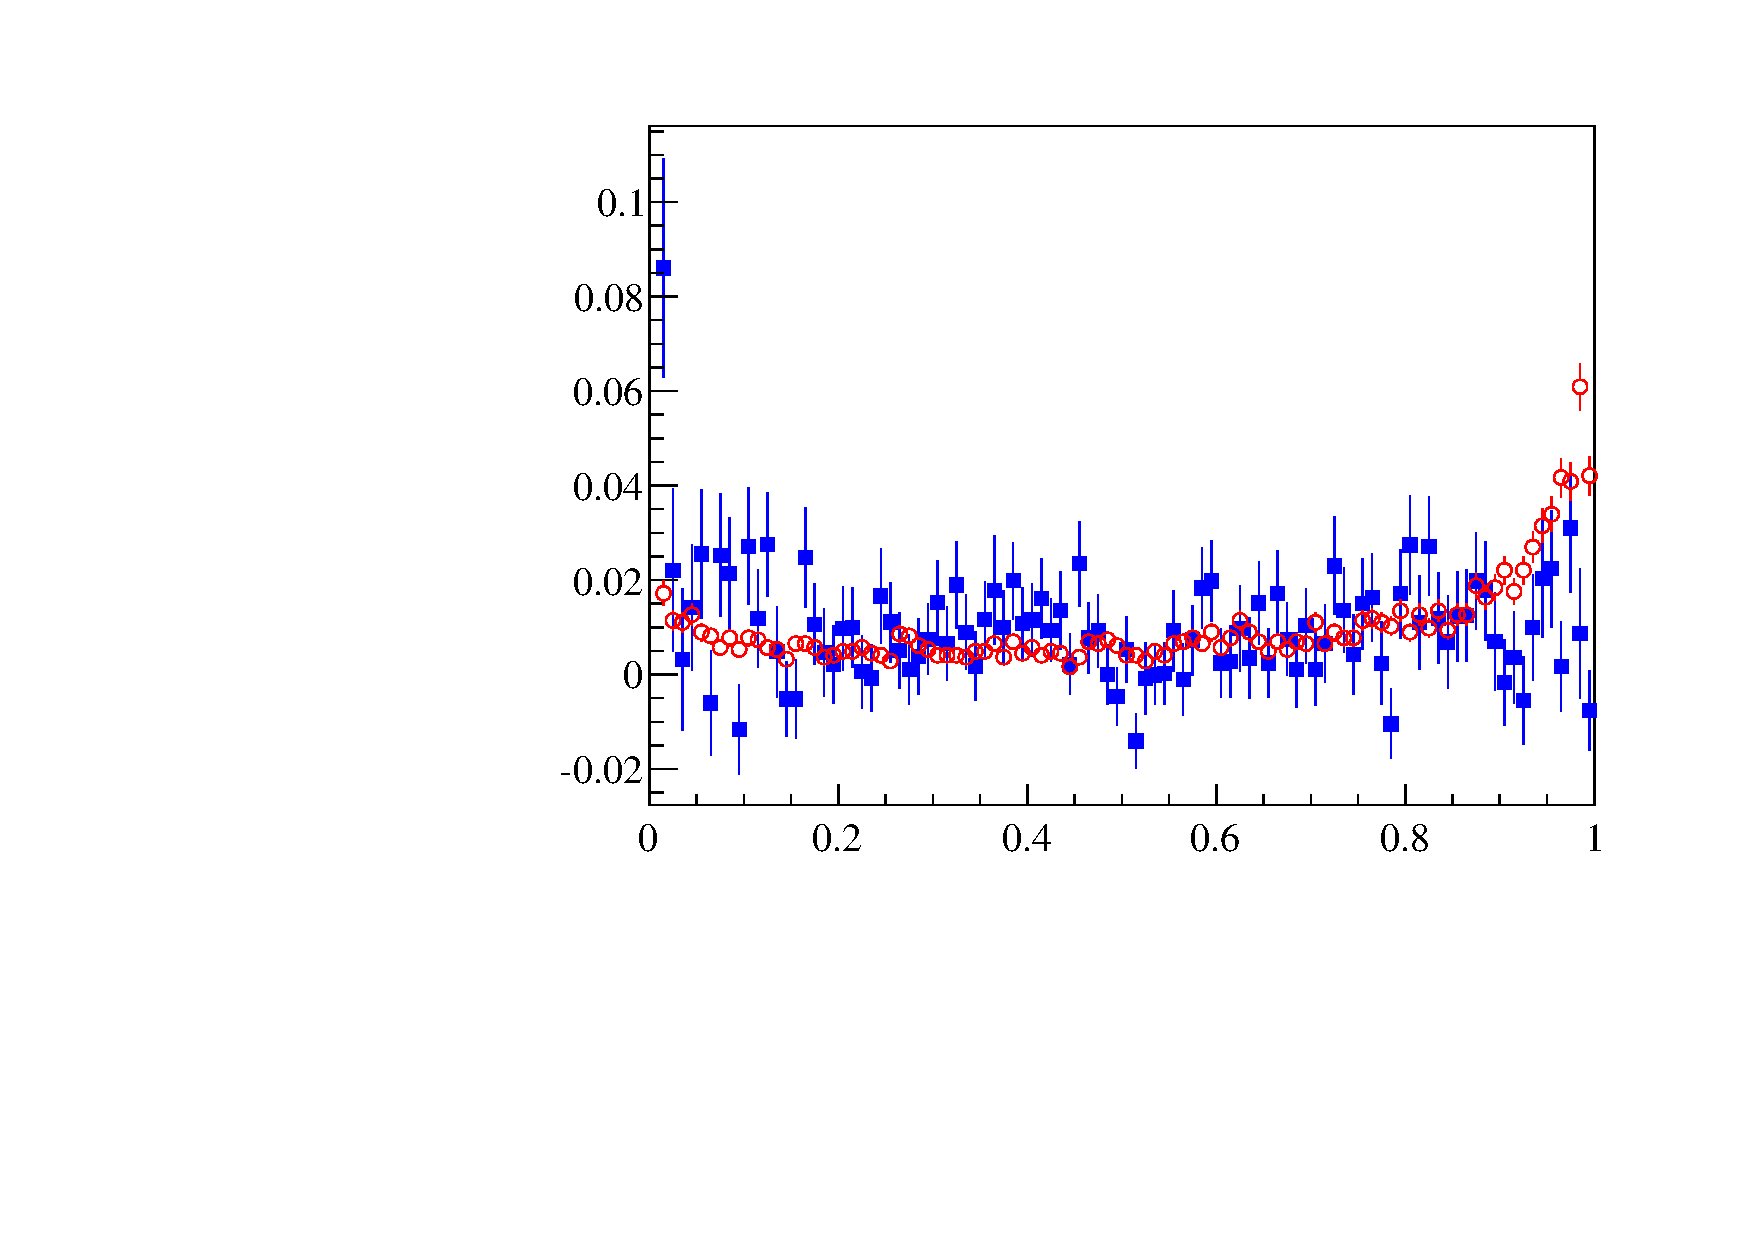
\includegraphics[width=50mm, height=35mm]{mc-data/cl_g_3p}
    }

    \put(0,35){
      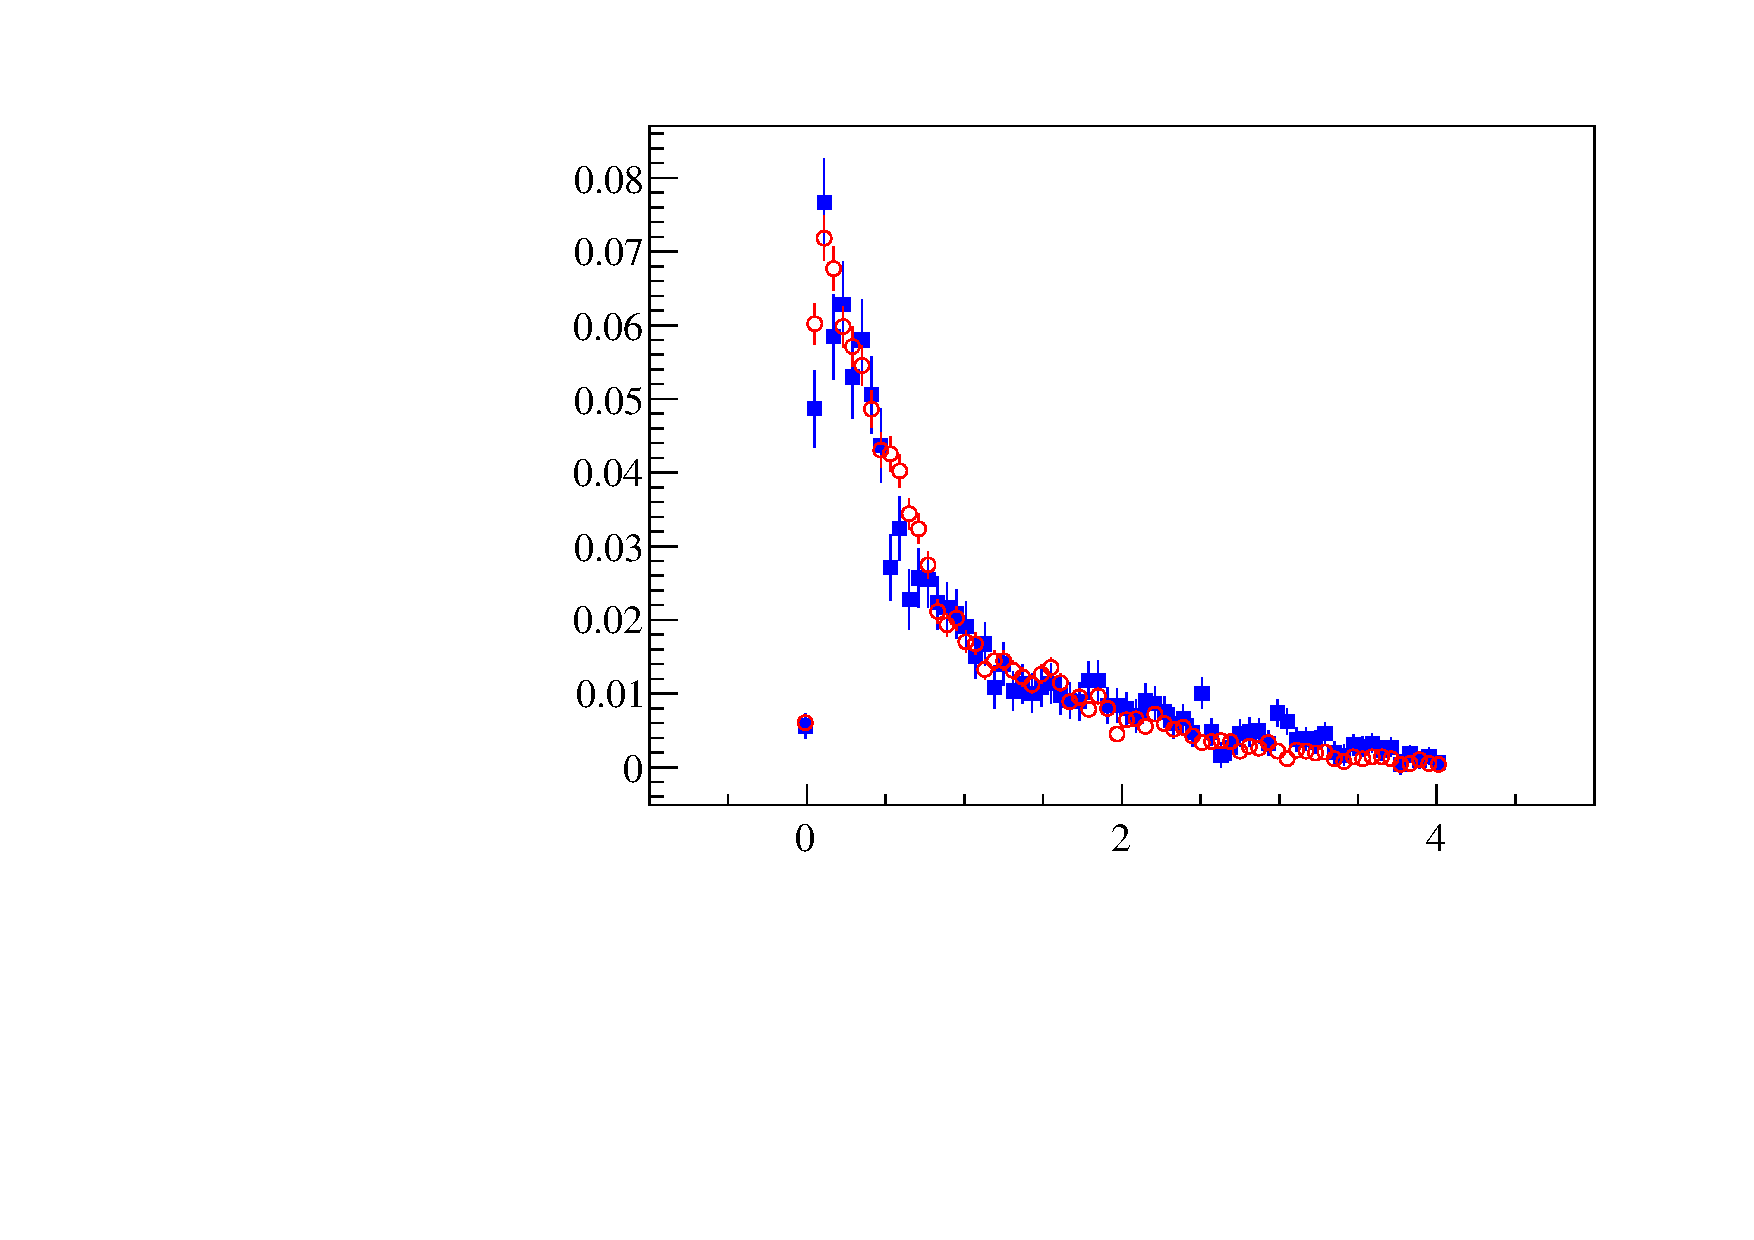
\includegraphics[width=50mm, height=35mm]{mc-data/c2_dtf_1p}
    }
    \put(50,35){
      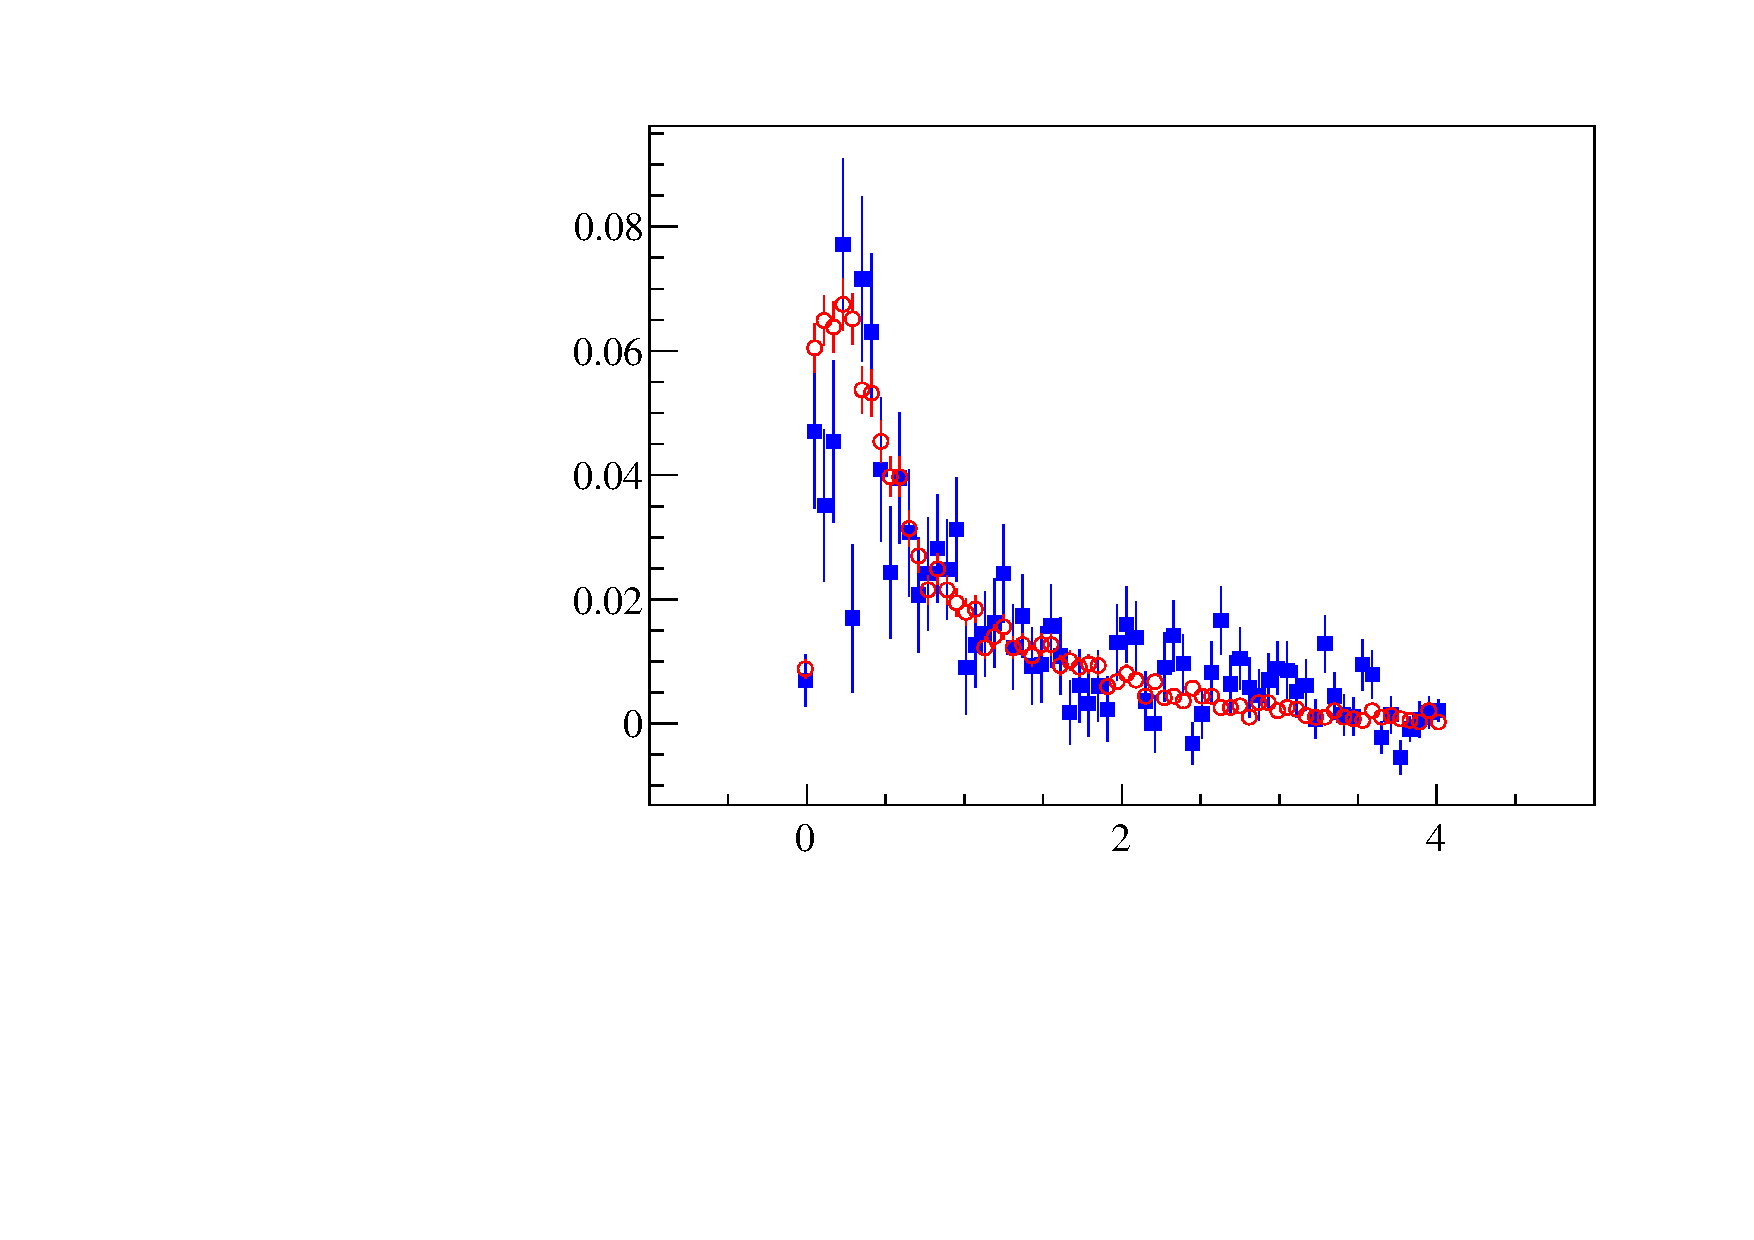
\includegraphics[width=50mm, height=35mm]{mc-data/c2_dtf_2p}
    }
    \put(100,35){
      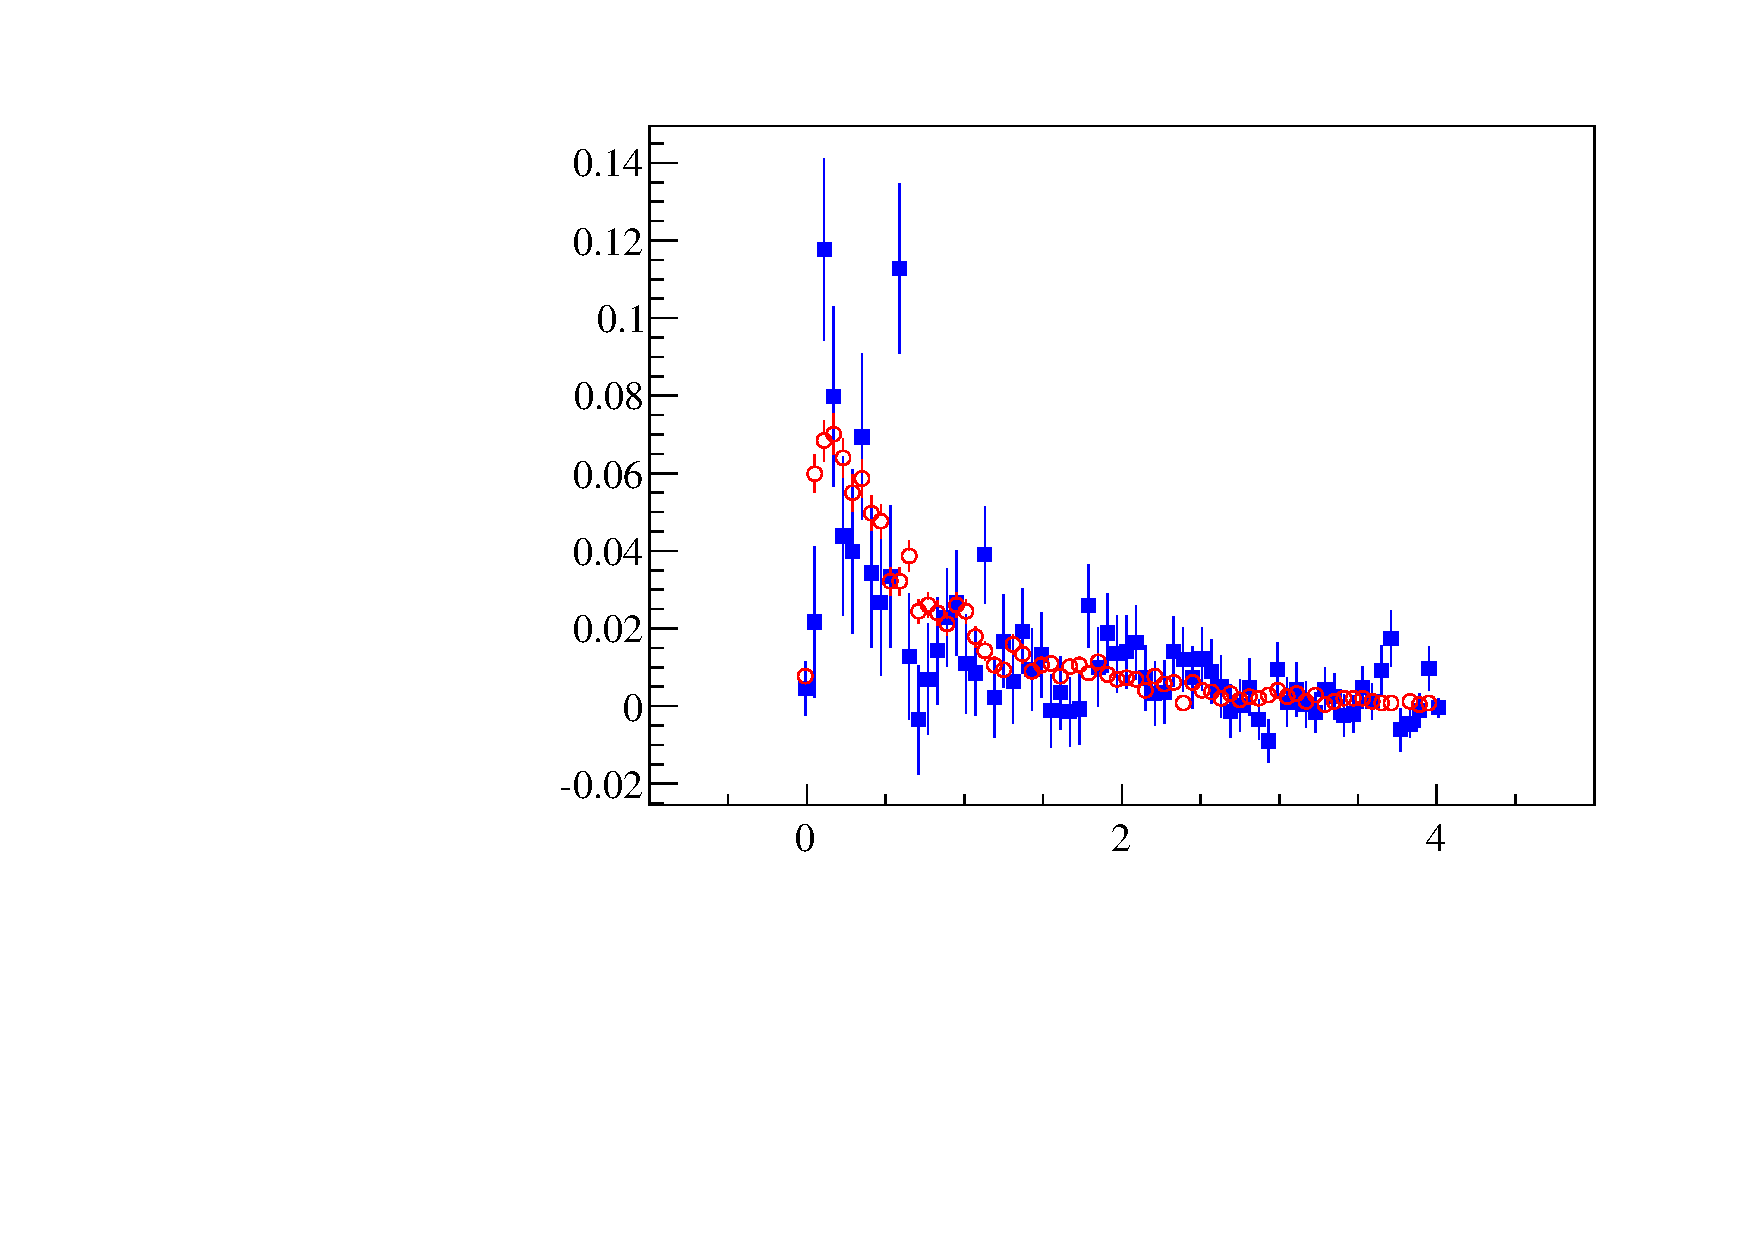
\includegraphics[width=50mm, height=35mm]{mc-data/c2_dtf_3p}
    }
    \put(0,70){
      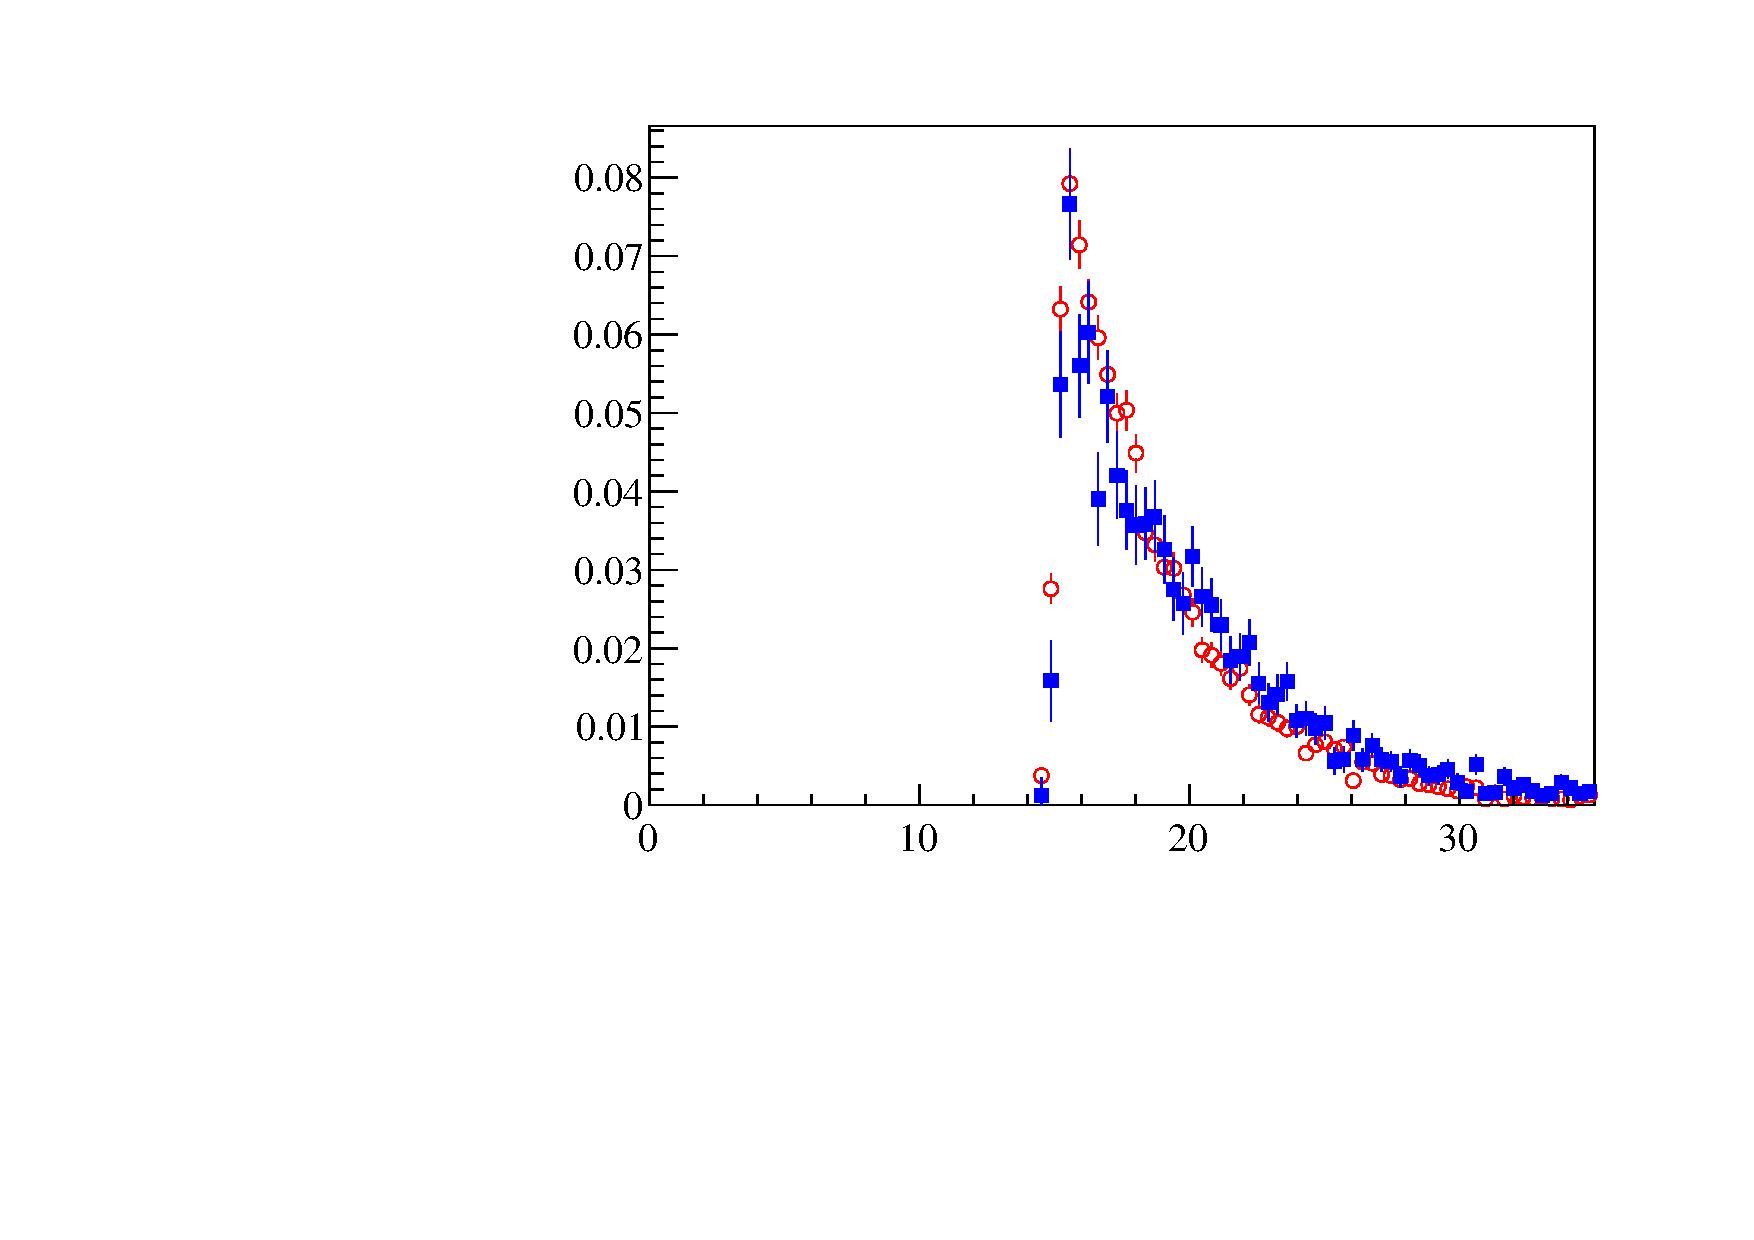
\includegraphics[width=50mm, height=35mm]{mc-data/pt_chib_1p}
    }
    \put(50,70){
      \includegraphics[width=50mm, height=35mm]{mc-data/pt_chib_2p}
    }
    \put(100,70){
      \includegraphics[width=50mm, height=35mm]{mc-data/pt_chib_3p}
    }
    \put(0,105){
      \includegraphics[width=50mm, height=35mm]{mc-data/pt_ups_1p}
    }
    \put(50,105){
      \includegraphics[width=50mm, height=35mm]{mc-data/pt_ups_2p}
    }
    \put(100,105){
      \includegraphics[width=50mm, height=35mm]{mc-data/pt_ups_3p}
    }

    \put(15,-1){\scriptsize $\gamma$ confidence level}
    \put(65,-1){\scriptsize $\gamma$ confidence level}
    \put(115,-1){\scriptsize $\gamma$ confidence level}
    \put(10,34){\scriptsize $\chisq$ of decay tree fitter}
    \put(60,34){\scriptsize $\chisq$ of decay tree fitter}
    \put(110,34){\scriptsize $\chisq$ of decay tree fitter}
    \put(20,69){\scriptsize $p_T[\chibOneP] \left[\gevcc\right]$}
    \put(70,69){\scriptsize $p_T[\chibTwoP] \left[\gevcc\right]$}
    \put(120,69){\scriptsize $p_T[\chibThreeP] \left[\gevcc\right]$}
    \put(20,104){\scriptsize $p_T[\Y1S] \left[\gevcc\right]$}
    \put(70,104){\scriptsize $p_T[\Y1S] \left[\gevcc\right]$}
    \put(120,104){\scriptsize $p_T[\Y1S] \left[\gevcc\right]$}

    \put(0,7){\scriptsize \begin{sideways}Arbitrary units\end{sideways}}
    \put(50,7){\scriptsize \begin{sideways}Arbitrary units\end{sideways}}
    \put(100,7){\scriptsize \begin{sideways}Arbitrary units\end{sideways}}
    \put(0,42){\scriptsize \begin{sideways}Arbitrary units\end{sideways}}
    \put(50,42){\scriptsize \begin{sideways}Arbitrary units\end{sideways}}
    \put(100,42){\scriptsize \begin{sideways}Arbitrary units\end{sideways}}
    \put(0,77){\scriptsize \begin{sideways}Arbitrary units\end{sideways}}
    \put(50,77){\scriptsize \begin{sideways}Arbitrary units\end{sideways}}
    \put(100,77){\scriptsize \begin{sideways}Arbitrary units\end{sideways}}
    \put(0,112){\scriptsize \begin{sideways}Arbitrary units\end{sideways}}
    \put(50,112){\scriptsize \begin{sideways}Arbitrary units\end{sideways}}
    \put(100,112){\scriptsize \begin{sideways}Arbitrary units\end{sideways}}

    \put(35,27){\scriptsize \chibOneP}
    \put(85,27){\scriptsize \chibTwoP}
    \put(135,27){\scriptsize \chibThreeP}
    \put(35,62){\scriptsize \chibOneP}
    \put(85,62){\scriptsize \chibTwoP}
    \put(135,62){\scriptsize \chibThreeP}
    \put(35,97){\scriptsize \chibOneP}
    \put(85,97){\scriptsize \chibTwoP}
    \put(135,97){\scriptsize \chibThreeP}
    \put(35,132){\scriptsize \chibOneP}
    \put(85,132){\scriptsize \chibTwoP}
    \put(135,132){\scriptsize \chibThreeP}
 
    % \graphpaper[5](0,0)(150, 175)        
  \end{picture}
}
\end{center}
\begin{block}{}
The agreement is generally very good.
\end{block}

\end{frame}

\begin{frame}{Monte-Carlo photon reconstruction efficiency}
\setlength{\unitlength}{1mm}
\begin{center}

\textcolor{blue}{\chibOneP}, \textcolor{red}{\chibTwoP}, \textcolor{cyan}{\chibThreeP} reconstruction efficiency in $\chib \to \Upsilon \gamma$ decays.

\begin{picture}(100,40)
      %
    \put(0,0){
      \includegraphics[width=50mm, height=40mm]{mc-eff/cb_ups1s}
    }
    \put(50,0){
      \includegraphics[width=50mm, height=40mm]{mc-eff/cb_ups2s}
    }
    
    \put(2,12){\begin{sideways}Efficiency (\%)\end{sideways}}
    \put(12,0){$p_T(\Y1S) \left[\gevcc\right]$}
    \put(10,35){\tiny $\chi_b(1,2,3P) \to \Y1S \gamma$}

    \put(52,12){\begin{sideways}Efficiency (\%)\end{sideways}}
    \put(62,0){$p_T(\Y2S) \left[\gevcc\right]$}
    \put(60,35){\tiny $\chi_b(2,3P) \to \Y2S \gamma$}


%    
%    \put(0,55){\tiny \begin{sideways}Candidates/(20\mevcc)\end{sideways}}
%    \put(2, 49.5){\tiny $m_{\mumu \gamma} - m_{\mumu} + 10.3552 \left[\gevcc\right]$}
%    \put(25,70){$\sqrt{s} = 7 \gev$}     
%    \graphpaper[2](0,0)(100, 40)        
  \end{picture}
 \end{center}
\begin{block}{}
Photons is more energetic as $p_T(\Upsilon)$ increases so it is reconstructed more efficiently.
\end{block}

\end{frame}
\begin{frame}[t]{The fraction of $\Upsilon$ originating from \chib decays}

\begin{columns}[t]
\column{.6\textwidth}

  \setlength{\unitlength}{1mm}
  \scalebox{0.42}{
  \begin{picture}(150,180)
    %% =======================================================================
    \put(0,120){
      \includegraphics[width=75mm, height=60mm]{frac-1s/cb1p_ups1s_2010}
    }
    \put(2,145){\begin{sideways}\Y1S fraction, \% \end{sideways}}
    \put(35,122){$p_T^{\Y1S} \left[\gevc\right]$}

    \put(45,173){\scriptsize $\chibOneP \to \Y1S \gamma$}
    \put(48,168){\scriptsize \textcolor{blue}{\sqs=7\tev}}
    \put(48,164){\scriptsize \textcolor{red}{\sqs=8\tev}}
    \put(48,160){\scriptsize \textcolor{cyan}{\sqs=7\tev (2010)}}
    
    \put(43,168){\includegraphics[width=3mm, height=2mm]{bsf}}
    \put(43,164){\includegraphics[width=3mm, height=2mm]{rco}}
    \put(43,160){\includegraphics[width=3mm, height=2mm]{ctuc}}
    %% =======================================================================
    \put(75,120){
      \includegraphics[width=75mm, height=60mm]{frac-1s/cb2p_ups1s}
    }
    \put(77,145){\begin{sideways}\Y1S fraction, \% \end{sideways}}
    \put(110,122){$p_T^{\Y1S} \left[\gevc\right]$}

    \put(120,173){\scriptsize $\chibTwoP \to \Y1S \gamma$}
    \put(123,168){\scriptsize \textcolor{blue}{\sqs=7\tev}}
    \put(123,164){\scriptsize \textcolor{red}{\sqs=8\tev}}
    
    
    \put(118,168){\includegraphics[width=3mm, height=2mm]{bsf}}
    \put(118,164){\includegraphics[width=3mm, height=2mm]{rco}}
    
    %% =======================================================================
    \put(0,60){
      \includegraphics[width=75mm, height=60mm]{frac-1s/cb3p_ups1s}
    }
    \put(2,85){\begin{sideways}\Y1S fraction, \% \end{sideways}}
    \put(35,62){$p_T^{\Y1S} \left[\gevc\right]$}

    \put(45,113){\scriptsize $\chibThreeP \to \Y1S \gamma$}
    \put(48,108){\scriptsize \textcolor{blue}{\sqs=7\tev}}
    \put(48,104){\scriptsize \textcolor{red}{\sqs=8\tev}}
    
    
    \put(43,108){\includegraphics[width=3mm, height=2mm]{bsf}}
    \put(43,104){\includegraphics[width=3mm, height=2mm]{rco}}
    
    %% =======================================================================
    \put(75,60){
      \includegraphics[width=75mm, height=60mm]{frac-1s/cb2p_ups2s}
    }
    \put(77,85){\begin{sideways}\Y2S fraction, \% \end{sideways}}
    \put(110,62){$p_T^{\Y2S} \left[\gevc\right]$}

    \put(120,113){\scriptsize $\chibTwoP \to \Y2S \gamma$}
    \put(123,108){\scriptsize \textcolor{blue}{\sqs=7\tev}}
    \put(123,104){\scriptsize \textcolor{red}{\sqs=8\tev}}
    
    
    \put(118,108){\includegraphics[width=3mm, height=2mm]{bsf}}
    \put(118,104){\includegraphics[width=3mm, height=2mm]{rco}}
    
    %% =======================================================================
    \put(0,0){
      \includegraphics[width=75mm, height=60mm]{frac-1s/cb3p_ups2s}
    }
    \put(2,25){\begin{sideways}\Y2S fraction, \% \end{sideways}}
    \put(35,2){$p_T^{\Y2S} \left[\gevc\right]$}

    \put(45,53){\scriptsize $\chibThreeP \to \Y2S \gamma$}
    \put(48,48){\scriptsize \textcolor{blue}{\sqs=7\tev}}
    \put(48,44){\scriptsize \textcolor{red}{\sqs=8\tev}}
    
    
    \put(43,48){\includegraphics[width=3mm, height=2mm]{bsf}}
    \put(43,44){\includegraphics[width=3mm, height=2mm]{rco}}
    
  % \graphpaper[5](0,0)(75, 60)
  \end{picture}
 }

\column{.4\textwidth}
\begin{itemize}
\item For $\chi_b(1P)$ decay the fraction is consistent with the previous
results.
 \item About 40\% of $\Upsilon$ come from $\chib$, with a mild transverse
 momentum dependence.
\item $\chi_b(3P)$ fraction in $\Upsilon(3S)$ decay is $34 \pm 7$ \% for
$24<p_T^{\Upsilon(3S)}<40\gevc$.
\end{itemize}
\end{columns}


\end{frame}
% \input{9.2-frac-2s}
% \input{9.3-frac-3s}
\begin{frame}{Systematic uncertainties due to $\lambda=N_{\chi_{b1}}/(N_{\chi_{b1}}+N_{\chi_{b2}})$ ratio in $\chi_b(1,2,3P) \to \OneS \gamma$ decays}
\begin{center}
\scalebox{0.4}{
\begin{tabular}{crrrrrrrrrrrrrrrr}\toprule
& \multicolumn{ 16 }{c}{\OneS transverse momentum intervals} \\
 & & \multicolumn{3}{c}{$6 < p_T < 8 \gevc$} & & \multicolumn{3}{c}{$8 < p_T < 10 \gevc$} & & \multicolumn{3}{c}{$10 < p_T < 12 \gevc$} & & \multicolumn{3}{c}{$12 < p_T < 14 \gevc$} \\
\cmidrule{3-5}\cmidrule{7-9}\cmidrule{11-13}\cmidrule{15-17}
$\lambda$ / Change (\%)  & & $N_{\chibOneP}$ & $N_{\chibTwoP}$ & $N_{\chibThreeP}$ & & $N_{\chibOneP}$ & $N_{\chibTwoP}$ & $N_{\chibThreeP}$ & & $N_{\chibOneP}$ & $N_{\chibTwoP}$ & $N_{\chibThreeP}$ & & $N_{\chibOneP}$ & $N_{\chibTwoP}$ & $N_{\chibThreeP}$ \\
\midrule
0.0  &  & 19 & -9 & -  &  & 24 & -3 & -  &  & 24 & -20 & -  &  & 16 & -1 & -6\\
0.1  &  & 13 & -8 & -  &  & 18 & -3 & -  &  & 18 & -17 & -  &  & 12 & -2 & -4\\
0.2  &  & 8 & -5 & -  &  & 12 & -2 & -  &  & 12 & -13 & -  &  & 8 & -2 & -2\\
0.3  &  & 4 & -4 & -  &  & 7 & -2 & -  &  & 7 & -9 & -  &  & 5 & -2 & -1\\
0.4  &  & 2 & -3 & -  &  & 3 & -1 & -  &  & 3 & \textcolor{red}{-5} & -  &  & 2 & -2 & 0\\
0.5  &  & 0 & -2 & -  &  & 0 & 0 & -  &  & 1 & -3 & -  &  & 1 & -1 & 1\\
0.6  &  & 0 & 1 & -  &  & -1 & 1 & -  &  & 0 & 0 & -  &  & 0 & 0 & 1\\
0.7  &  & 1 & -1 & -  &  & -1 & 1 & -  &  & 0 & 1 & -  &  & 0 & 2 & 0\\
0.8  &  & 3 & -2 & -  &  & 0 & 1 & -  &  & 2 & 2 & -  &  & 1 & 4 & 0\\
0.9  &  & 7 & -5 & -  &  & 3 & 1 & -  &  & 5 & 1 & -  &  & 3 & 6 & -1\\
1.0  &  & 10 & -9 & -  &  & 6 & 1 & -  &  & 9 & 0 & -  &  & 5 & 9 & -2\\
\bottomrule
\end{tabular}
}


\scalebox{0.35}{
\begin{tabular}{crrrrrrrrrrrrrrrr}\toprule
& \multicolumn{ 16 }{c}{\OneS transverse momentum intervals} \\
 & & \multicolumn{3}{c}{$14 < p_T < 18 \gevc$} & & \multicolumn{3}{c}{$18 < p_T < 22 \gevc$} & & \multicolumn{3}{c}{$22 < p_T < 30 \gevc$} & & \multicolumn{3}{c}{$18 < p_T < 30 \gevc$} \\
\cmidrule{3-5}\cmidrule{7-9}\cmidrule{11-13}\cmidrule{15-17}
$\lambda$ / Change (\%)  & & $N_{\chibOneP}$ & $N_{\chibTwoP}$ & $N_{\chibThreeP}$ & & $N_{\chibOneP}$ & $N_{\chibTwoP}$ & $N_{\chibThreeP}$ & & $N_{\chibOneP}$ & $N_{\chibTwoP}$ & $N_{\chibThreeP}$ & & $N_{\chibOneP}$ & $N_{\chibTwoP}$ & $N_{\chibThreeP}$ \\
\midrule
0.0  &  & 15 & 1 & -14 &  & 12 & 0 & -5 &  & 9 & -5 & -11 &  & 11 & -2 & -8\\
0.1  &  & 11 & 0 & -10 &  & 8 & -1 & -3 &  & 6 & -4 & -9 &  & 7 & -2 & -5\\
0.2  &  & 7 & 0 & -6 &  & 5 & -1 & -1 &  & 3 & -4 & -6 &  & 4 & -2 & -3\\
0.3  &  & \textcolor{red}{4} & -1 & -3 &  & 2 & -1 & 0 &  & 1 & -3 & -4 &  & 2 & -2 & -1\\
0.4  &  & 2 & -1 & -1 &  & 1 & -1 & 0 &  & 0 & -2 & \textcolor{red}{-3} &  & 0 & -1 & 0\\
0.5  &  & 0 & -1 & 1 &  & 0 & -1 & 0 &  & -1 & -1 & -1 &  & 0 & 0 & 1\\
0.6  &  & 0 & 0 & 1 &  & 0 & 0 & 0 &  & 0 & 0 & 0 &  & 0 & 0 & 1\\
0.7  &  & 1 & 0 & 1 &  & 1 & 1 & -1 &  & 1 & 1 & 1 &  & 1 & 1 & 1\\
0.8  &  & 2 & 2 & 0 &  & 2 & 2 & -3 &  & 4 & 2 & 2 &  & 3 & 3 & 0\\
0.9  &  & 4 & 3 & -1 &  & 5 & 4 & -3 &  & 7 & 3 & 2 &  & 6 & 5 & 0\\
1.0  &  & 7 & 5 & -2 &  & 8 & 7 & -4 &  & 10 & 5 & 3 &  & 9 & 7 & 0\\
\bottomrule
\end{tabular}
}

\begin{block}{}
Theory predicts lambda in range [0.4,0.6]. When varying lambda in this range, the maximum uncertainty on the yields is 4\%, 5\% and 3\% for $N_{\chibOneP}$, $N_{\chibTwoP}$ and $N_{\chibThreeP}$, respectively.
\end{block}

\end{center}
\end{frame}
\begin{frame}{Systematic uncertainties due to $\lambda=N_{\chi_{b1}}/(N_{\chi_{b1}}+N_{\chi_{b2}})$ ratio in $\chi_b(2,3P) \to \TwoS \gamma$ decays}
\begin{center}
\scalebox{0.7}{
\begin{tabular}{crrrrrr}\toprule
& \multicolumn{ 6 }{c}{\TwoS transverse momentum intervals} \\
 & & \multicolumn{2}{c}{$18 < p_T < 25 \gevc$} & & \multicolumn{2}{c}{$25 < p_T < 40 \gevc$} \\
\cmidrule{3-4}\cmidrule{6-7}
$\lambda$ / Change (\%)  & & $N_{\chibTwoP}$ & $N_{\chibThreeP}$ & & $N_{\chibTwoP}$ & $N_{\chibThreeP}$ \\
\midrule
0.0  &  & 12 & 10 &  & 12 & -4\\
0.1  &  & 7 & 6 &  & 8 & -3\\
0.2  &  & 4 & 3 &  & 6 & -7\\
0.3  &  & 1 & 1 &  & 3 & -5\\
0.4  &  & 0 & 0 &  & 1 & -3\\
0.5  &  & 0 & 0 &  & 0 & 0\\
0.6  &  & 1 & 1 &  & \textcolor{red}{-2} & \textcolor{red}{11}\\
0.7  &  & 4 & 4 &  & 1 & 8\\
0.8  &  & 7 & 8 &  & 3 & 12\\
0.9  &  & 11 & 13 &  & 6 & 17\\
1.0  &  & 17 & 19 &  & 10 & 22\\
\bottomrule
\end{tabular}
}
\end{center}

\begin{block}{}
Theory predicts lambda in range [0.4,0.6]. When varying lambda in this range, the maximum uncertainty on the yields is 2\% and 11\% for $N_{\chibTwoP}$ and $N_{\chibThreeP}$, respectively.
\end{block}
\end{frame}
\begin{frame}{ Systematic uncertainties due to $m_{\chiboneOneP}$ mass range in $\chi_b(1,2,3P) \to \OneS \gamma$ decays.}
Uncertainty due to the $\chiboneOneP$ mass variation in the $p_T^{\OneS}$ range is estimated by using the observed minimum and maximum values.

\begin{center}
\scalebox{0.4}{
\begin{tabular}{crrrrrrrrrrrrrrrr}\toprule
& \multicolumn{ 16 }{c}{\OneS transverse momentum intervals} \\
 & & \multicolumn{3}{c}{$6 < p_T < 8 \gevc$} & & \multicolumn{3}{c}{$8 < p_T < 10 \gevc$} & & \multicolumn{3}{c}{$10 < p_T < 12 \gevc$} & & \multicolumn{3}{c}{$12 < p_T < 14 \gevc$} \\
\cmidrule{3-5}\cmidrule{7-9}\cmidrule{11-13}\cmidrule{15-17}
$\m(\chiboneOneP)$ / Change (\%)  & & $N_{\chibOneP}$ & $N_{\chibTwoP}$ & $N_{\chibThreeP}$ & & $N_{\chibOneP}$ & $N_{\chibTwoP}$ & $N_{\chibThreeP}$ & & $N_{\chibOneP}$ & $N_{\chibTwoP}$ & $N_{\chibThreeP}$ & & $N_{\chibOneP}$ & $N_{\chibTwoP}$ & $N_{\chibThreeP}$ \\
\midrule
9.885 \gevcc ($min\left[m(\chiboneOneP)\right]$) &  & -1 & 0 & -  &  & \textcolor{red}{-6} & 2 & -  &  & 0 & 5 & -  &  & -2 & \textcolor{red}{6} & 1\\
9.896 \gevcc ($max\left[m(\chiboneOneP)\right]$) &  & 4 & -1 & -  &  & 6 & -1 & -  &  & 4 & -5 & -  &  & 3 & -2 & -1\\
\bottomrule
\end{tabular}
}

\scalebox{0.4}{
\begin{tabular}{crrrrrrrrrrrrrrrr}\toprule
& \multicolumn{ 16 }{c}{\OneS transverse momentum intervals} \\
 & & \multicolumn{3}{c}{$14 < p_T < 18 \gevc$} & & \multicolumn{3}{c}{$18 < p_T < 22 \gevc$} & & \multicolumn{3}{c}{$22 < p_T < 30 \gevc$} & & \multicolumn{3}{c}{$18 < p_T < 30 \gevc$} \\
\cmidrule{3-5}\cmidrule{7-9}\cmidrule{11-13}\cmidrule{15-17}
$\m(\chiboneOneP)$ / Change (\%)  & & $N_{\chibOneP}$ & $N_{\chibTwoP}$ & $N_{\chibThreeP}$ & & $N_{\chibOneP}$ & $N_{\chibTwoP}$ & $N_{\chibThreeP}$ & & $N_{\chibOneP}$ & $N_{\chibTwoP}$ & $N_{\chibThreeP}$ & & $N_{\chibOneP}$ & $N_{\chibTwoP}$ & $N_{\chibThreeP}$ \\
\midrule
9.885 \gevcc ($min\left[m(\chiboneOneP)\right]$) &  & -1 & 2 & 4 &  & 1 & 4 & -2 &  & 3 & 5 & \textcolor{red}{8} &  & 2 & 5 & 2\\
9.896 \gevcc ($max\left[m(\chiboneOneP)\right]$) &  & 2 & 0 & -3 &  & 1 & 0 & 1 &  & 0 & -2 & -5 &  & 1 & -2 & -2\\
\bottomrule
\end{tabular}
}
\end{center}
\begin{block}{}
Maximum uncertainty on the yields is 6\%, 6\% and 8\% for $N_{\chibOneP}$,
$N_{\chibTwoP}$ and $N_{\chibThreeP}$, respectively.
\end{block}

\end{frame}
\begin{frame}{Systematic uncertainties due to $m_{\chiboneTwoP}$ mass range $\chi_b(2,3P) \to \TwoS \gamma$ decays}

Uncertainty due to the $\chiboneTwoP$ mass variation in the $p_T^{\TwoS}$ range is estimated by using the observed minimum and maximum values.

\begin{center}

\scalebox{0.7}{
\begin{tabular}{crrrrrr}\toprule
& \multicolumn{ 6 }{c}{\TwoS transverse momentum intervals} \\
 & & \multicolumn{2}{c}{$18 < p_T < 25 \gevc$} & & \multicolumn{2}{c}{$25 < p_T < 40 \gevc$} \\
\cmidrule{3-4}\cmidrule{6-7}
$\m(\chiboneTwoP)$ / Change (\%)  & & $N_{\chibTwoP}$ & $N_{\chibThreeP}$ & & $N_{\chibTwoP}$ & $N_{\chibThreeP}$ \\
\midrule
10.245 \gevcc ($min\left[m_{\chiboneTwoP}\right]$) &  & 4 & 4 &  & -2 & \textcolor{red}{19}\\
10.255 \gevcc ($max\left[m_{\chiboneTwoP}\right]$) &  & 3 & 2 &  & \textcolor{red}{8} & -11\\
\bottomrule
\end{tabular}
}
\end{center}
\begin{block}{}
Maximum uncertainty on the yields is 8\% and 19\% for 
$N_{\chibTwoP}$ and $N_{\chibThreeP}$, respectively.
\end{block}
\end{frame}
\begin{frame}{ Systematic uncertainties due to $m_{\chiboneThreeP}$ mass range in $\chi_b(1,2,3P) \to \OneS \gamma$  and 
    $\chi_b(2,3P) \to \TwoS \gamma$ decays
}

Uncertainty due to the $\chiboneThreeP$ mass variation in the $p_T^{\Upsilon}$
range is estimated by using the observed minimum and maximum values.

\begin{center}

\scalebox{0.4}{
\begin{tabular}{crrrrrrrrrrrrrrrr}\toprule
& \multicolumn{ 16 }{c}{\OneS transverse momentum intervals} \\
 & & \multicolumn{3}{c}{$14 < p_T < 18 \gevc$} & & \multicolumn{3}{c}{$18 < p_T < 22 \gevc$} & & \multicolumn{3}{c}{$22 < p_T < 30 \gevc$} & & \multicolumn{3}{c}{$18 < p_T < 30 \gevc$} \\
\cmidrule{3-5}\cmidrule{7-9}\cmidrule{11-13}\cmidrule{15-17}
$\m(\chiboneThreeP)$ / Change (\%)  & & $N_{\chibOneP}$ & $N_{\chibTwoP}$ & $N_{\chibThreeP}$ & & $N_{\chibOneP}$ & $N_{\chibTwoP}$ & $N_{\chibThreeP}$ & & $N_{\chibOneP}$ & $N_{\chibTwoP}$ & $N_{\chibThreeP}$ & & $N_{\chibOneP}$ & $N_{\chibTwoP}$ & $N_{\chibThreeP}$ \\
\midrule
10.503 \gevcc ($min\left[m(\chiboneThreeP)\right]$) &  & 0 & -1 & -6 &  & 0 & 1 & 7 &  & 0 & 0 & 1 &  & 0 & 1 & 5\\
10.517 \gevcc ($max\left[m(\chiboneThreeP)\right]$) &  & 0 & \textcolor{red}{3} & \textcolor{red}{19} &  & 0 & -2 & -14 &  & 0 & 0 & -2 &  & 0 & -1 & -9\\
\bottomrule
\end{tabular}
}

\begin{block}{}
Maximum uncertainty on the yields is 3\% and 19\% for $N_{\chibTwoP}$ an $N_{\chibThreeP}$, respectively.
\end{block}

\vspace{0.5in}

\scalebox{0.5}{
\begin{tabular}{crrrrrr}\toprule
& \multicolumn{ 6 }{c}{\TwoS transverse momentum intervals} \\
 & & \multicolumn{2}{c}{$18 < p_T < 25 \gevc$} & & \multicolumn{2}{c}{$25 < p_T < 40 \gevc$} \\
\cmidrule{3-4}\cmidrule{6-7}
$\m(\chiboneThreeP)$ / Change (\%)  & & $N_{\chibTwoP}$ & $N_{\chibThreeP}$ & & $N_{\chibTwoP}$ & $N_{\chibThreeP}$ \\
\midrule
10.503 \gevcc ($min\left[m(\chiboneThreeP)\right]$) &  & 0 & -1 &  & 0 & -4\\
10.517 \gevcc ($max\left[m(\chiboneThreeP)\right]$) &  & 0 & 4 &  & 0 & \textcolor{red}{-8}\\
\bottomrule
\end{tabular}
}

\begin{block}{}
Maximum uncertainty on the yields is 8\% for $N_{\chibThreeP}$.
\end{block}

\end{center}
\end{frame}
\begin{frame}{Systematic uncertainties due to $\chib$ polarization}
\begin{block}{}
\small
Efficiencies are evaluated on MC where chib particles are unpolarized. To evaluate systematic effects due to the unknown polarization of chib, MC events are reweighted as described in \textcolor{blue}{HERA-B Collaboration, I. Abt et al.,  Production of the Charmonium States $\chi_{c1}$ and $\chi_{c2}$ in Proton Nucleus Interactions at s = 41.6-GeV}, \href{http://arxiv.org/abs/0807.2167}{arXiv:0807.2167} and
\textcolor{blue}{LHCb collaboration, R. Aaij et al.,Measurement of the cross-section ratio $\sigma(\chi_{c2})/\sigma(\chi_{c1})$ for prompt $\chi_c$
production at $\sqrt{s}=7$ TeV}, \href{http://arxiv.org/abs/1202.1080}{arXiv:1202.1080}
\end{block}
For each simulated event in the unpolarised sample, a weight is calculated from
the distribution of the following angles in the various polarisation hypotheses compared to the
unpolarised distribution.

\scalebox{0.7}{
\begin{tabular}{c|p{10cm}}\toprule
$\Theta_{\Upsilon}$ & angle between the directions of the $\mu^{+}$ in the $\Upsilon$ rest frame and the $\Upsilon$ in the $\chi_b$ rest frame.\\
\midrule
$\Theta_{\chi_b}$ & angle between the directions of the $\Upsilon$ in the $\chi_b$ rest frame and $\chi_b$ in the lab frame.\\
\midrule
$\phi$ & angle between the $\Upsilon$ decay plane in the $\chi_b$ rest frame and the plane formed by $\chi_b$ direction in the lab frame and the direction of the $\Upsilon$ in the $\chi_b$ rest frame.\\
\bottomrule
\end{tabular}
}

\vspace{0.1in}

Two hypotheses for $\chibone$ state (w0, w1) and three hypotheses for $\chibtwo$ (w0, w1, w2).

\end{frame}
\begin{frame}{Systematic uncertainties due to \chib polarization}
The ratio of efficiency for unpolarized \chib to efficiency for polarized \chib.

\includegraphics[width=40mm, height=25mm]{syst-pol/chib21p_ups1s_w0_ratio.pdf}
\includegraphics[width=40mm, height=25mm]{syst-pol/chib21p_ups1s_w1_ratio.pdf}
\includegraphics[width=40mm, height=25mm]{syst-pol/chib21p_ups1s_w2_ratio.pdf}

\begin{block}{}
The efficiency in the different polarization scenarios is consistent with the unpolarized one. We conservatively take the statistical uncertainty on the efficiency ratio as systematic uncertainty due to the chib polarization.
\end{block}

\end{frame}
\begin{frame}{Summary}

\begin{itemize}
\item Measured fractions of \Y1,2,3S originated from \chib decays.
About 40\% of $\Upsilon$ come from $\chi_b$, with mild dependence on $\Upsilon$ transverse momentum.
\item Measured mass of $\chi_b(3P)$ is 10507$\pm$2\mevcc, consistent with another determination which uses converted photons.
\end{itemize}

\begin{block}{}
An LHCb internal note documenting this study has been written. The analysis is currently under 
internal review and will be the subject of an LHCb publication.
\end{block}

\end{frame}


% \begin{frame}[t]{Backup}
% \end{frame}




\end{document}
